% A LaTeX template for ARTICLE version of the MSc Thesis submissions to 
% Politecnico di Milano (PoliMi) - School of Industrial and Information Engineering
%
% S. Bonetti, A. Gruttadauria, G. Mescolini, A. Zingaro
% e-mail: template-tesi-ingind@polimi.it
%
% Last Revision: October 2021
%
% Copyright 2021 Politecnico di Milano, Italy. Inc. NC-BY

\documentclass[11pt,a4paper]{article} 

%------------------------------------------------------------------------------
%	REQUIRED PACKAGES AND  CONFIGURATIONS
%------------------------------------------------------------------------------
% PACKAGES FOR TITLES
\usepackage{titlesec}
\usepackage{xcolor}

% PACKAGES FOR LANGUAGE AND FONT
\usepackage[utf8]{inputenc}
\usepackage[english]{babel}
\usepackage[T1]{fontenc} % Font encoding

% PACKAGES FOR IMAGES
\usepackage{graphicx}
\usepackage[space]{grffile}
\graphicspath{{Images/}}
\usepackage{eso-pic} % For the background picture on the title page
\usepackage{subfig} % Numbered and caption subfigures using \subfloat
\usepackage{caption} % Coloured captions
\usepackage{transparent}

% STANDARD MATH PACKAGES
\usepackage{amsmath}
\usepackage{amsthm}
\usepackage{bm}
\usepackage[overload]{empheq}  % For braced-style systems of equations
\usepackage{amssymb}

% PACKAGES FOR TABLES
\usepackage{tabularx}
\usepackage{longtable} % tables that can span several pages
\usepackage{colortbl}
\usepackage{multirow}

% PACKAGES FOR ALGORITHMS (PSEUDO-CODE)
\usepackage{algorithm}
\usepackage{algorithmic}

% PACKAGES FOR REFERENCES & BIBLIOGRAPHY
\usepackage[colorlinks=true,linkcolor=black,anchorcolor=black,citecolor=black,filecolor=black,menucolor=black,runcolor=black,urlcolor=black]{hyperref} % Adds clickable links at references
\usepackage{cleveref}
\usepackage[square, numbers, sort&compress]{natbib} % Square brackets, citing references with numbers, citations sorted by appearance in the text and compressed
\bibliographystyle{plain} % You may use a different style adapted to your field

% PACKAGES FOR THE APPENDIX
\usepackage{appendix}

% PACKAGES FOR ITEMIZE & ENUMERATES 
\usepackage{enumitem}

% OTHER PACKAGES
\usepackage{thmtools} % Coloured "Theorem"
\usepackage{comment} % Comment part of code
\usepackage{fancyhdr} % Fancy headers and footers
\usepackage{lipsum} % Insert dummy text
\usepackage{tcolorbox} % Create coloured boxes (e.g. the one for the key-words)

%added by me
\usepackage{tabularray}
\usepackage{float}
%-------------------------------------------------------------------------
%	NEW COMMANDS DEFINED
%-------------------------------------------------------------------------
% EXAMPLES OF NEW COMMANDS -> here you see how to define new commands
\newcommand{\bea}{\begin{eqnarray}} % Shortcut for equation arrays
\newcommand{\eea}{\end{eqnarray}}
\newcommand{\e}[1]{\times 10^{#1}}  % Powers of 10 notation
\newcommand{\mathbbm}[1]{\text{\usefont{U}{bbm}{m}{n}#1}} % From mathbbm.sty
\newcommand{\pdev}[2]{\frac{\partial#1}{\partial#2}}
% NB: you can also override some existing commands with the keyword \renewcommand

%----------------------------------------------------------------------------
%	ADD YOUR PACKAGES (be careful of package interaction)
%----------------------------------------------------------------------------


%----------------------------------------------------------------------------
%	ADD YOUR DEFINITIONS AND COMMANDS (be careful of existing commands)
%----------------------------------------------------------------------------


% Do not change Configuration_files/config.tex file unless you really know what you are doing. 
% This file ends the configuration procedures (e.g. customizing commands, definition of new commands)
% Configuration package
\usepackage{lmodern}
\usepackage[bottom=2.0cm,top=2.0cm,left=2.0cm,right=2.0cm]{geometry}
\raggedbottom 

% Create color bluePoli (-> manuale grafica coordinata:  https://www.polimi.it/fileadmin/user_upload/il_Politecnico/grafica-coordinata/2015_05_11_46xy_manuale_grafica_coordinata.pdf)
\definecolor{bluePoli}{cmyk}{0.4,0.1,0,0.4}

% Custom theorem environments
\declaretheoremstyle[
  headfont=\color{bluePoli}\normalfont\bfseries,
  bodyfont=\color{black}\normalfont\itshape,
]{colored}

\captionsetup[figure]{labelfont={color=bluePoli}} % Set colour of the captions
\captionsetup[table]{labelfont={color=bluePoli}} % Set colour of the captions
%\captionsetup[algorithm]{labelfont={color=bluePoli}} % Set colour of the captions

\theoremstyle{colored}
\newtheorem{theorem}{Theorem}[section]
\newtheorem{proposition}{Proposition}[section]

% Enhances the features of the standard "table" and "tabular" environments.
\newcommand\T{\rule{0pt}{2.6ex}}
\newcommand\B{\rule[-1.2ex]{0pt}{0pt}}

% Algorithm description
\newcounter{algsubstate}
\renewcommand{\thealgsubstate}{\alph{algsubstate}}
\newenvironment{algsubstates}{
    \setcounter{algsubstate}{0}%
    \renewcommand{\STATE}{%
    \stepcounter{algsubstate}%
    \Statex {\small\thealgsubstate:}\space}
    }{}
    
% Custom theorem environment
\newcolumntype{L}[1]{>{\raggedright\let\newline\\\arraybackslash\hspace{0pt}}m{#1}}
\newcolumntype{C}[1]{>{\centering\let\newline\\\arraybackslash\hspace{0pt}}m{#1}}
\newcolumntype{R}[1]{>{\raggedleft\let\newline\\\arraybackslash\hspace{0pt}}m{#1}}

% Custom itemize environment
\setlist[itemize,1]{label=$\bullet$}
\setlist[itemize,2]{label=$\circ$}
\setlist[itemize,3]{label=$-$}
\setlist{nosep}

% Create command for background pic
\newcommand\BackgroundPic{% Adding background picture
	\put(237,365){
	    \parbox[b][\paperheight]{\paperwidth}{%
	    \vfill
		\centering
		\transparent{0.4}
		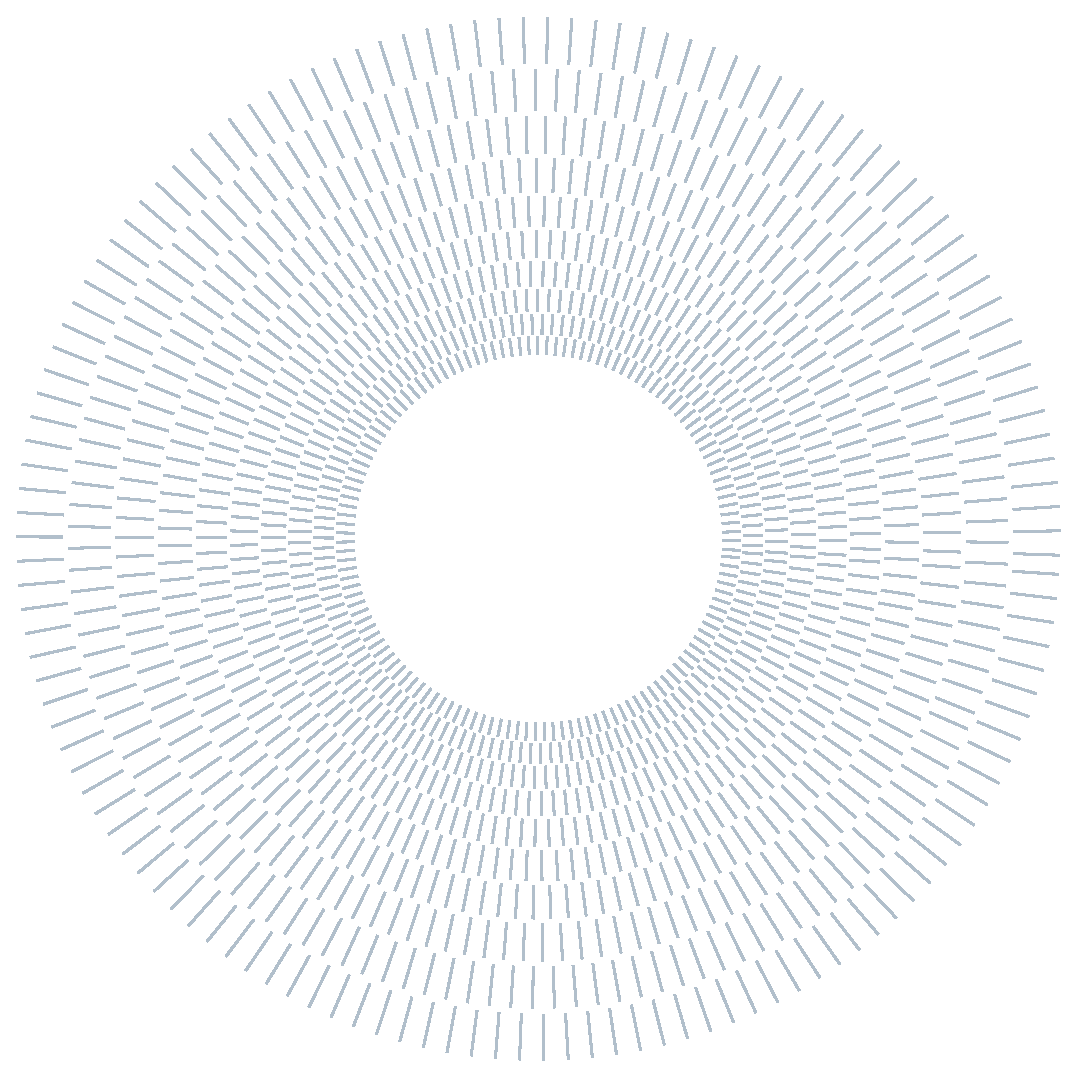
\includegraphics[width=0.44\paperwidth]{raggiera_polimi.eps}%
		\vfill}
		}
}

% Set indentation
\setlength\parindent{0pt}

% Custom title commands
\titleformat{\section}
{\color{bluePoli}\normalfont\Large\bfseries}
{\color{bluePoli}\thesection.}{1em}{}
\titlespacing*{\section}
{0pt}{3.3ex}{3.3ex}

\titleformat{\subsection}
{\color{bluePoli}\normalfont\large\bfseries}
{\color{bluePoli}\thesubsection.}{1em}{}
\titlespacing*{\subsection}
{0pt}{3.3ex}{3.3ex}

% Custom headers and footers
\pagestyle{fancy}
\fancyhf{}
      
\fancyfoot{}
\fancyfoot[C]{\thepage} % page
\renewcommand{\headrulewidth}{0mm} % headrule width
\renewcommand{\footrulewidth}{0mm} % footrule width

\makeatletter
\patchcmd{\headrule}{\hrule}{\color{black}\hrule}{}{} % headrule
\patchcmd{\footrule}{\hrule}{\color{black}\hrule}{}{} % footrule
\makeatother

% Insert here the info that will be displayed into your Title page 
% -> title of your work
\renewcommand{\title}{Intra-Sequence Synthesis of MRI Images via Generative AI Methods}
% -> author name and surname
\renewcommand{\author}{Pietro Filippo Schgor}
% -> MSc course
\newcommand{\course}{Mathematical Engineering - Ingegneria Matematica}
% -> advisor name and surname
\newcommand{\advisor}{Prof. Lara Cavinato}
% IF AND ONLY IF you need to modify the co-supervisors you also have to modify the file Configuration_files/title_page.tex (ONLY where it is marked)
\newcommand{\firstcoadvisor}{Luca Caldera} % insert if any otherwise comment
% -> author ID
\newcommand{\ID}{258727}
% -> academic year
\newcommand{\YEAR}{2025-2026}
% -> abstract (only in English)
\renewcommand{\abstract}{Multi-modal Magnetic Resonance Imaging (MRI), comprising T1-weighted, T2-weighted, and FLAIR sequences, is essential for accurate neurological diagnosis, yet acquiring a complete protocol is frequently impeded by prolonged scan times, patient motion, and limited scanner availability. This thesis presents a systematic benchmark of three 3D generative architectures for intra-modal MRI synthesis: Pix2Pix, Edge-Aware GAN (EA-GAN), and Pyramid Transformer Network (PTNet3D). All models were trained on the ADNI dataset using a patch-based strategy and evaluated on both internal and external multi-center cohorts (IXI and OpenNeuro) through a comprehensive suite of voxel-level, structural, and perceptual metrics. Results show that the CNN-based architectures—particularly EA-GAN—consistently achieve superior intra-domain synthesis fidelity, with EA-GAN excelling in perceptual and structural metrics such as SSIM, LPIPS, and FSIM. Conversely, the transformer-based PTNet3D, despite lower absolute intensity accuracy and higher computational cost, demonstrates remarkable robustness to domain shift. The clinical utility of the synthesized volumes is further validated through two downstream tasks: brain age estimation on the IXI dataset and epilepsy classification (healthy controls vs. focal cortical dysplasia) on the OpenNeuro dataset. These results reveal a key trade-off between local synthesis precision and cross-domain generalization, and confirm that current 3D generative architectures can produce clinically viable synthetic MRI volumes.}

% -> key-words (only in English)
\newcommand{\keywords}{Magnetic Resonance Imaging (MRI), Generative Adversarial Networks (GANs), 3D Image-to-Image Translation, Pix2Pix, EA-GAN, PTNet3D, Transformers, Neuroimaging}

%-------------------------------------------------------------------------
%	BEGIN OF YOUR DOCUMENT
%-------------------------------------------------------------------------
\begin{document}

%-----------------------------------------------------------------------------
% TITLE PAGE
%-----------------------------------------------------------------------------
% Do not change Configuration_files/TitlePage.tex (Modify it IF AND ONLY IF you need to add or delete the Co-advisors)
% This file creates the Title Page of the document
% DO NOT REMOVE SPACES BETWEEN LINES!

\AddToShipoutPicture*{\BackgroundPic}

\hspace{-0.6cm}
\includegraphics[width=0.6\textwidth]{logo_polimi_ing_indinf.eps}

\vspace{-1mm}
\Large{\textbf{\color{bluePoli}{\title}}}

\vspace{-0.2cm}
\fontsize{0.3cm}{0.5cm}\selectfont \textsc{\color{bluePoli} Tesi di Laurea Magistrale in \\ \course}

\vspace{-0.2cm}
\large{\textbf{\author, \ID}}

\small \normalfont

\vspace{11pt}

\centerline{\rule{1.0\textwidth}{0.4pt}}

\begin{center}
\begin{minipage}[t]{.24\textwidth}
\begin{minipage}{.90\textwidth}
\noindent
\scriptsize
\textbf{Advisor:} \\
\advisor \\[1ex]
\textbf{Co-advisors:} \\ % leave it if any co-advisor otherwise comment
\firstcoadvisor \\[1ex] % leave it if any co-advisor otherwise comment
%\secondcoadvisor \\ % leave it if you have more that one co-advisor otherwise comment (if you have more than two co-advisors just copy&paste this line writing \thirdcoadvisor, \fourthcoadvisor, ecc. (REMEMBER to modify also the main.txt)
\textbf{Academic year:} \\
\YEAR
\end{minipage}
\end{minipage}% This must go next to \end{minipage}
\begin{minipage}{.74\textwidth}
\noindent \textbf{\color{bluePoli} Abstract:} {\abstract}
\end{minipage}
\end{center}

\vspace{15pt}

\begin{tcolorbox}[arc=0pt, boxrule=0pt, colback=bluePoli!60, width=\textwidth, colupper=white]
    \textbf{Key-words:} \keywords
\end{tcolorbox}

\vspace{12pt}


%%%%%%%%%%%%%%%%%%%%%%%%%%%%%%
%%     THESIS MAIN TEXT     %%
%%%%%%%%%%%%%%%%%%%%%%%%%%%%%%

%-----------------------------------------------------------------------------
% INTRODUCTION
%-----------------------------------------------------------------------------
\section{Introduction}
\label{sec:introduction}

Medical imaging, particularly magnetic resonance imaging (MRI), plays a critical role in clinical diagnostics by providing distinct visual representations of anatomy and soft tissue structures through task-specific scanning parameters \cite{CLARKE1995343, AD1999}. In neuroimaging, different MRI sequences---such as T1-weighted, T2-weighted, and FLAIR---serve complementary roles. When analyzed collectively, these multi-modal images enhance predictive power for studying neuroanatomy \cite{7898360}, planning therapies \cite{7738594}, and segmenting brain lesions \cite{HAVAEI201718, kamnitsas_ledig_newcombe_simpson_kane_menon_rueckert_glocker_2017}. 

Despite these clinical benefits, acquiring a full multi-sequence protocol is frequently hindered by practical limitations: factors such as prolonged scan times, patient motion, acoustic noise, high costs, and limited scanner availability often preclude ubiquitous multi-modal imaging. Furthermore, modality inconsistency between different clinical centers exacerbates this issue \cite{chartsias2018}. Consequently, the clinical demand for comprehensive multi-modal analysis is often unmet, which can adversely affect the quality of diagnosis and treatment.

To address these constraints, medical image synthesis has emerged as a highly valuable solution. By defining a nonlinear mapping from available source-modality images to unknown target-modality images, learning-based methods can bypass the costs and times associated with additional scans \cite{10.1007/978-3-642-40811-3_79, huo2018}. The clinical value of this intra-modal synthesis is significant: it enables the imputation of corrupted or missing sequences, accelerates acquisition protocols, and provides robust data augmentation for downstream deep learning tasks. 

The primary objective of this thesis is to systematically benchmark three distinct generative architectures for intra-modal MRI translation, specifically mapping between T1, T2, and FLAIR sequences. Pix2Pix, EA-GAN, and PTNet3D were specifically selected for this comparative analysis due to their native capacity to process 3D volumetric inputs and directly generate corresponding 3D outputs. By comparing these specific models across both internal and external cohorts, this work highlights the architectural evolution---from traditional convolutional constraints to edge-aware losses and advanced long-range attention mechanisms---within a fully three-dimensional framework leveraging a patch-based volumetric inference strategy.

As a crucial secondary contribution, this thesis moves beyond standard image similarity metrics by directly assessing the clinical utility and diagnostic validity of the synthesized scans in downstream applications. Specifically, we investigate how the introduction of synthetic data, both independently and in hybrid augmentation regimes, impacts model performance across two fundamental machine learning paradigms: a regression task (brain age estimation) and a binary classification task (epilepsy detection via focal cortical dysplasia identification). By demonstrating that synthetic data can effectively preserve task-relevant anatomical features and measurably enhance downstream predictive accuracy, this work provides strong empirical support for the practical adoption of intra-sequence synthesis, underscoring the vital necessity of deploying reliable, anatomically faithful generative models in clinical workflows.


The remainder of this thesis is organized as follows. Chapter~\ref{sec: 2} reviews the theoretical foundations of deep learning for image-to-image translation alongside the current state-of-the-art literature in intra-modal MRI synthesis. Chapter~\ref{sec: 3} details the multi-site dataset cohorts, the preprocessing pipeline, and the intensity normalization protocols. Chapter~\ref{sec: 4} presents the mathematical and architectural formulation of the benchmarked generative models in chronological order of their development. Subsequently, Chapter~\ref{sec: 5} outlines the experimental setup, detailing the training mechanics, implementation specifics, and the comprehensive suite of voxel-wise and perceptual evaluation metrics. Chapter~\ref{sec: 6} presents and discusses both quantitative and qualitative translation results, alongside localized error analyses and downstream validation on clinical regression and classification tasks. Finally, Chapter~\ref{sec: 7} summarizes the key findings of this work, critically discusses architectural and hardware limitations, and outlines promising future directions toward unified multi-domain and diffusion-based frameworks.




%-----------------------------------------------------------------------------
% CHAPTER 2
%-----------------------------------------------------------------------------

\section{Background \& Related Work}
\label{sec: 2}

\subsection{MRI Sequences and Tissue Contrast}
Magnetic Resonance Imaging exploits the response of hydrogen nuclei (protons) to radiofrequency pulses within a strong static magnetic field. After excitation, tissue magnetization recovers along two independent time courses---longitudinal relaxation ($T_1$) and transverse relaxation ($T_2$)---whose rates depend on the local molecular environment. By varying the echo time (TE) and repetition time (TR), the specific MRI sequence can weight the acquired signal to emphasize one relaxation mechanism over the other, producing distinct \textit{contrast profiles} for the same anatomy \cite{AD1999}.

\paragraph{T1-Weighted Imaging}
A T1-weighted (T1w) sequence acquisition employs a short TR and short TE, thereby maximizing the contrast driven by longitudinal relaxation differences. Fat-rich tissues and myelinated white matter (WM) appear hyperintense (bright), whereas cerebrospinal fluid (CSF) and cortical grey matter (GM) appear relatively dark. T1w scans are the standard reference for structural neuroimaging due to their excellent grey--white matter contrast.

\paragraph{T2-Weighted Imaging}
A T2-weighted (T2w) sequence acquisition uses a long TR and long TE to emphasize transverse relaxation. The resulting contrast is approximately the inverse of T1w: CSF and water-rich tissues appear bright, while WM appears dark. T2w images are particularly valuable for detecting pathological processes such as oedema, inflammation, and demyelination, which typically increase local water content.

\paragraph{FLAIR Imaging}
Fluid-Attenuated Inversion Recovery (FLAIR) is a T2-weighted variant in which an inversion pulse is applied to null the signal from free water, effectively suppressing the bright CSF signal. This suppression dramatically improves the conspicuity of periventricular and subcortical white-matter lesions---such as those caused by multiple sclerosis, small-vessel disease, or focal cortical dysplasia---which would otherwise be masked by the adjacent, similarly bright CSF on standard T2w images.
\medskip
 
Because each sequence highlights different tissue properties, the joint availability of T1w, T2w, and FLAIR images provides complementary diagnostic information. However, acquiring all three sequences for every patient is often impractical (see Section~\ref{sec:introduction}), which motivates the intra-modal synthesis framework developed in this thesis.

\subsection{Early Approaches and CNN-based Synthesis}
Driven by its remarkable success in solving inverse problems, deep learning has been rapidly adopted across the field of medical imaging \cite{review_1, review_2}. Due to the fact that target images must be predicted without access to corresponding target-modality data, medical image synthesis represents a distinctly ill-posed challenge \cite{nie2018}. Initial investigations into this area primarily relied on local networks utilizing patch-level processing \cite{hien2015, li2014, torrado2016}. Although these local approaches provided advantages over conventional techniques, their ability to capture broader contextual information across entire images remained constrained \cite{sevetlidis2016}.

As large-scale imaging databases became increasingly available, subsequent research shifted toward deep CNNs for full image-level processing. The efficacy of CNN-based synthesis has been proven across multiple domains, such as cross-scanner MR translation \cite{behrami2016, bahrami2016b, nie2018, zhang2019}, multi-contrast MRI synthesis \cite{bowles2016, chartsias2018, cordier2016, sevetlidis2016, joyce2017, wei2019}, and CT generation \cite{han2017, nie2016, arabi2018, klaser2019}. Nevertheless, despite the substantial advancements they introduced, CNNs relying solely on pixel-wise loss functions often fail to preserve intricate structural details \cite{pix2pix, cyclegan, pgan}.

\paragraph{Generative Adversarial Networks in Medical Imaging}
In order to better capture these structural nuances, Generative Adversarial Networks (GANs) \cite{gan} were introduced to model the target modality's distribution conditional on the source input \cite{conditionalgan}. By employing adversarial losses, GANs establish a stronger prior that facilitates the restoration of high-spatial-resolution features \cite{pix2pix, cyclegan, pgan}. Over recent years, GAN architectures have established state-of-the-art benchmarks in a wide array of synthesis applications, spanning from data augmentation to multi-modal generation \cite{sandfort2019, frida2018, pgan, lee2019}. Notable implementations of these models encompass translations from CT to PET \cite{bencohen2018, santini2020} and MR to CT \cite{jin2018, ge2019, woltering2017}, alongside unpaired cross-modality synthesis \cite{dong2019, yang2018, hiasa2018, chartsias2017}, 3T-to-7T upgrades \cite{huy2021, xiang2018}, and extensive multi-contrast MRI synthesis \cite{armanious2019, beers2018, pgan, scgan, lee2019, li2019, mmgan, wang2020, yang2021, yu2018, yu2019, yurt2021mustgan, zhou2020, nie2018}.

\paragraph{Structural and Edge-Aware Refinements: Pix2Pix and EA-GAN}
Within this landscape of adversarial models, \textbf{Pix2Pix} \cite{pix2pix} stood out as a pioneering architecture for medical image-to-image translation. Through the integration of a U-Net generator and a PatchGAN discriminator, it successfully maintained high-frequency structural integrity by merging adversarial training with an L1 reconstruction penalty. To further refine the preservation of delicate anatomical boundaries, \textbf{EA-GAN} (Edge-Aware GAN) \cite{yu2019} was developed as an enhancement to this convolutional baseline. By explicitly feeding structural edge data into the generative pipeline and deploying a multi-task loss function---which balances adversarial, perceptual, and edge-preservation constraints---EA-GAN produces highly realistic outputs characterized by precise tissue delineations.

\subsection{Overcoming Convolutional Limitations: Attention Mechanisms and Transformers}
Despite their current status as a gold standard, GAN models still present notable limitations. Their reliance on strictly convolutional operators often leads to sub-optimal modeling of long-range spatial dependencies and diminished generalization across subjects with atypical anatomies \cite{wang2018nonlocal, kodali2018}. To counter this, newer research has embedded spatial or channel attention mechanisms to dynamically adjust CNN-generated feature maps \cite{kearney2020, sagan, attention_unet, scgan, zhao2020, yuan2020, li2020}. This strategic modulation encourages the network to concentrate on areas prone to higher error rates \cite{sagan, attention_unet}. However, because this approach relies on the multiplicative gating of localized CNN features, its capacity to fully model global context remains restricted, even when attention maps are spread across the image \cite{xie2021, trans_unet, dai2021}.

Consequently, transformer-based techniques have garnered significant attention for their ability to integrate comprehensive contextual representations into imaging tasks, including segmentation \cite{trans_unet, xie2021, karimi2021}, reconstruction \cite{TransGAN, TransCT, SLATER}, and synthesis \cite{kamran2021, ganbert, ptnet3d}. While several independent studies have recently applied transformers to medical image synthesis---yielding models like VTGAN \cite{kamran2021} and GANBERT \cite{ganbert}---these initial iterations, along with hybrid frameworks like ResViT \cite{resvit}, frequently omit adversarial components or remain heavily dependent on purely convolutional generators.

\paragraph{Volumetric Attention and 3D Modeling: PTNet3D}
In response to the need for modeling long-range context within a native three-dimensional environment, architectures such as \textbf{PTNet3D} \cite{ptnet3d} were engineered. Employing a hybrid attention strategy, PTNet3D executes voxel-wise translations across different MRI sequences. By utilizing performer layers in its encoding and decoding stages, the model circumvents the quadratic computational burden typically associated with applying standard transformers to high-resolution 3D data. Simultaneously, it successfully retains global contextual dependencies by routing features through a central transformer bottleneck coupled with a multi-scale pyramid representation.

Through a comparative analysis of Pix2Pix, EA-GAN, and PTNet3D, this thesis evaluates the trajectory of architectural advancements in the field: tracing the evolution from conventional patch-based convolutional limits, through targeted edge-aware refinements, up to the deployment of sophisticated, fully 3D long-range attention systems.
%-----------------------------------------------------------------------------
% CHAPTER 3
%-----------------------------------------------------------------------------

\section{Datasets \& preprocessing}
\label{sec: 3}

\subsection{Datasets}
\label{subsec:datasets}
We obtained T1-weighted, T2-weighted, and Fluid-Attenuated Inversion Recovery (FLAIR) MR images from three distinct datasets. Specifically, the primary training set and an internal test set were extracted from the Alzheimer's Disease Neuroimaging Initiative (ADNI, combining ADNI3 and ADNI4 cohorts) \cite{jack2008alzheimer}, which provides all three MRI modalities. To rigorously evaluate the cross-domain generalization capabilities of our models, we additionally integrated two external test sets: the IXI Brain Development Dataset (IXI) \cite{ixidata} for the T1$\leftrightarrow$T2 translation task, and an OpenNeuro Dataset \cite{ds004199:1.0.0} for the T1$\leftrightarrow$FLAIR translation task.

These datasets inherently introduce significant domain variance due to both the diverse sequence acquisition equipment used and the varied clinical conditions of the participants. The ADNI cohort was acquired across multiple clinical sites utilizing 3.0T systems from three major manufacturers---General Electric (GE) Healthcare, Philips Healthcare, and Siemens Healthineers---and comprises older subjects aged $55$--$104$ years (mean $\pm$ standard deviation: $72.9 \pm 8.2$ years) spanning different cognitive stages: $56.9\%$ Cognitively Normal (CN), $29.7\%$ Mild Cognitive Impairment (MCI), $9.1\%$ Alzheimer's Disease (AD), and $4.3\%$ with unrecorded diagnostic status. In contrast, the IXI dataset consists entirely of healthy individuals (aged $28$--$95$ years) and was collected across three different hospitals in London utilizing three distinct scanners: a Philips 3.0T system at Hammersmith Hospital, a Philips 1.5T system at Guy's Hospital, and a GE 1.5T system at the Institute of Psychiatry. Conversely, the OpenNeuro dataset contains images acquired using a 3.0T Siemens MRI scanner from a younger cohort (aged $10$--$65$ years) perfectly balanced between healthy controls and patients diagnosed with Focal Cortical Dysplasia (FCD). Table~\ref{tab:datasets} summarizes the precise number of images available for each modality, the training and test splits, the scanner manufacturers, field strengths, participant age ranges, and clinical diagnostic statuses.

\begin{table}[H]
\centering
\scriptsize
\begin{tblr}{
  colsep = 3pt,
  colspec = {
    Q[l,m,2.0cm]
    Q[c,m,1.2cm]
    Q[c,m,1.1cm]
    Q[c,m,0.8cm]
    Q[c,m,0.8cm]
    Q[c,m,1.8cm]
    Q[c,m,1.5cm]
    Q[c,m,1.2cm]
    Q[c,m,2.4cm]
  }
}
\hline[0.5pt]
\textbf{Dataset} & \textbf{Modality} & \textbf{Training} & \textbf{Test} & \textbf{Total} & \textbf{Scanner} & \textbf{Field Strength} & \textbf{Age Range} & \textbf{Clinical Status} \\  
\hline \hline
\SetCell[r=3]{} \textbf{ADNI} \cite{jack2008alzheimer} & T1 & 1294 & 227 & 1521 & \SetCell[r=3]{} Philips, GE, Siemens & \SetCell[r=3]{} 3.0T & \SetCell[r=3]{} 55-104 & \SetCell[r=3]{} 56.9\% CN \newline 29.7\% MCI \newline 9.1\% AD \newline (4.3\% N/A) \\
& T2 & 405 & 90 & 495 & & & & \\
& FLAIR & 1290 & 222 & 1512 & & & & \\
\hline
\SetCell[r=2]{} \textbf{IXI} \cite{ixidata} & T1 & - & 581 & 581 & \SetCell[r=2]{} Philips, GE & \SetCell[r=2]{} 1.5T / 3.0T & \SetCell[r=2]{} 28-95 & \SetCell[r=2]{} Healthy \\
& T2 & - & 577 & 577 & & & & \\
\hline
\SetCell[r=2]{} \textbf{OpenNeuro} \cite{ds004199:1.0.0} & T1 & - & 170 & 170 & \SetCell[r=2]{} Siemens & \SetCell[r=2]{} 3.0T & \SetCell[r=2]{} 10-65 & \SetCell[r=2]{} 50\% Healthy \newline 50\% FCD \\
& FLAIR & - & 170 & 170 & & & & \\
\hline[0.5pt]
\end{tblr}
\caption{Datasets description, including training and test splits across different MRI modalities, total images, scanner manufacturers, field strengths, participant age range, and clinical status (CN: Cognitively Normal, MCI: Mild Cognitive Impairment, AD: Alzheimer's Disease, FCD: Focal Cortical Dysplasia).}
\label{tab:datasets}
\end{table}

\subsection{Preprocessing Steps}
\label{subsec:preprocessing}
Image preprocessing was conducted using the FSL library \citep{fsl1, fsl2}. Initially, the images were standardized to a common orientation. Next, bias-field correction was applied to address magnetic field variations in the MRI scanner, which can lead to blurring, loss of detail, and altered pixel intensities. The \texttt{FAST} algorithm within FSL was used for this correction, combining the non-parametric N3 bias field correction algorithm with a parametric model-based approach. The images were then registered to a standard space using the \texttt{FLIRT} command in FSL, which employs an affine transformation model to align the images through translations, rotations, and scaling, mapping them to the Standard MNI152-T1-1mm space. Following spatial normalization, the resulting images had dimensions of $(1, \ 182, \ 218, \ 182)$. Finally, to ensure numerical stability and compatibility with the adversarial learning frameworks, a global intensity normalization protocol was applied, linearly mapping the voxel intensities of all MR sequences into the strictly defined $[-1, 1]$ range before being fed to the generative networks.

%-----------------------------------------------------------------------------
% CHAPTER 4
%-----------------------------------------------------------------------------

\section{Models}
\label{sec: 4}

\subsection{Pix2Pix}

The Pix2Pix model, introduced by Isola et al. in 2017 \cite{pix2pix}, provides a general-purpose framework for image-to-image translation tasks based on Conditional Generative Adversarial Networks (cGANs). Unlike traditional GANs that generate images from random noise vectors, Pix2Pix learns a mapping from an observed input image to an output image. This conditional approach has proven highly effective for a wide array of tasks, such as synthesizing photographs from semantic label maps, reconstructing full-color images from grayscale inputs, and generating realistic objects from edge maps.

\subsubsection{Architecture}
The model consists of two primary, antagonistically trained components: a Generator ($G$) and a Discriminator ($D$).

\paragraph{Generator: 3D U-Net}
In many image translation tasks, the input and output images differ significantly in surface appearance but inherently share the same underlying spatial structure. To preserve this crucial structural information, Pix2Pix employs a \textbf{U-Net} architecture for the Generator, rather than a standard encoder-decoder network. 

The standard encoder-decoder compresses the input into a low-dimensional bottleneck, which can lead to a loss of low-level details (e.g., edges, fine textures). The U-Net overcomes this by introducing \textit{skip connections} between the layers of the encoder and the corresponding layers of the decoder. Specifically, a skip connection is added between layer $i$ and layer $n-i$, where $n$ is the total number of layers. These connections allow low-level structural information to bypass the bottleneck, enabling the generation of high-resolution, structurally accurate details.

The overall architectural scheme of the 3D U-Net generator, reproduced from the Ea-GAN framework \cite{yu2019}, is illustrated in Figure~\ref{fig:unet_pix2pix}. In our 3D volumetric adaptation, the encoder consists of $7$ downsampling steps utilizing 3D Convolutions with a kernel size of $4 \times 4 \times 4$, a stride of $2$, and a padding of $1$. Each convolutional layer is followed by 3D Instance Normalization and a LeakyReLU ($0.2$) activation. The base number of feature maps starts at $64$, progressively doubling up to $512$ at the bottleneck. The decoding path mirrors the encoder, employing 3D Transposed Convolutions, standard ReLU activations, and Instance Normalization. As depicted in the schematic, skip connections transfer feature representations from the contracting path to the expanding path via copy and concatenation. Furthermore, to prevent overfitting and encourage stochasticity, Dropout with a probability of $0.5$ is applied to the innermost decoder layers. The generator takes a single-channel 3D input volume and outputs the synthesized target volume.

\begin{figure}[htbp]
    \centering
    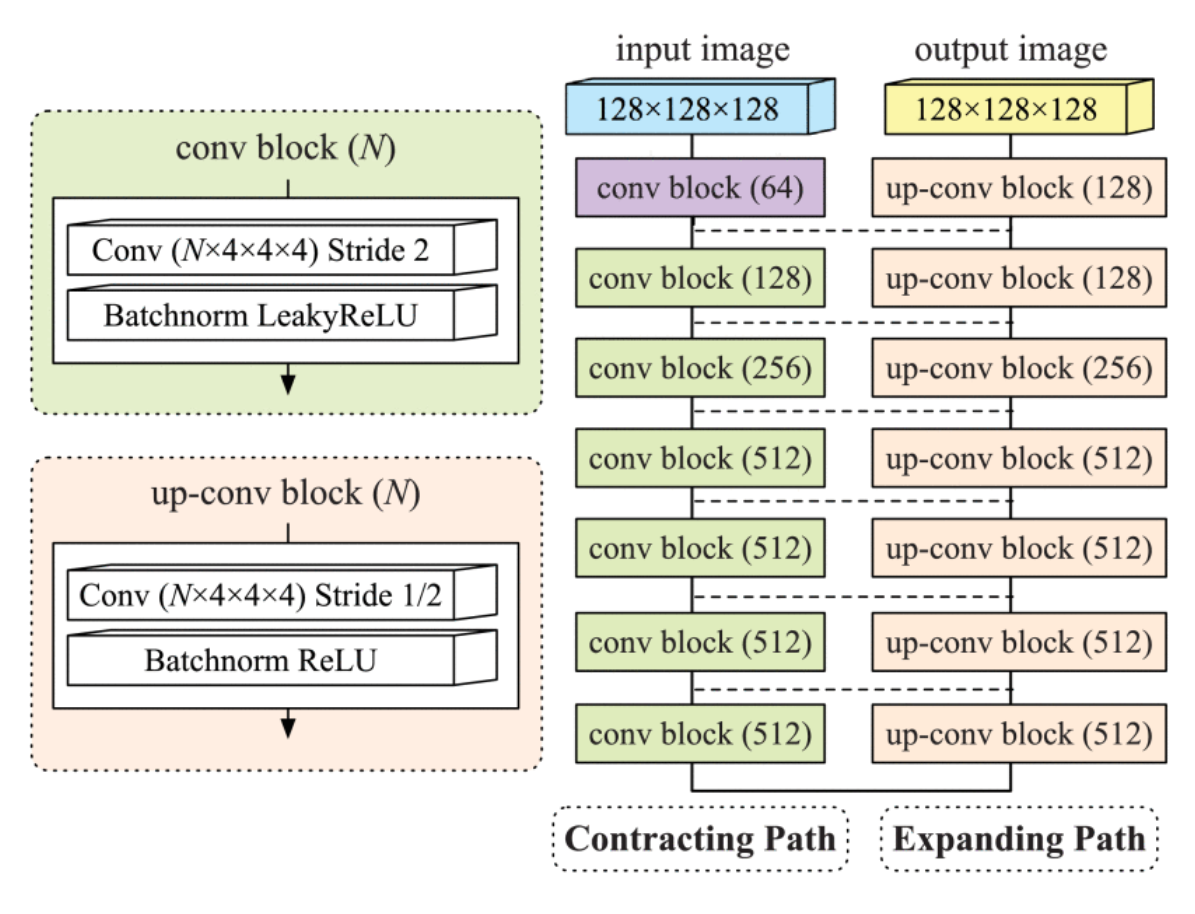
\includegraphics[width=0.7\textwidth]{Images/EAGAN-PIX2PIX GENERATOR.png}
    \caption{The 3D U-Net Generator architecture (reproduced from \cite{yu2019}). All conv and up-conv blocks contain convolutional, instance normalization, and activation layers. Dropout is applied to the first three blocks on the expanding path. Instance normalization is not used in the first block of the contracting path. Dashed lines denote the skip connections between contracting and expanding paths by copy and concatenation. The slope of LeakyReLUs is $0.2$.}
    \label{fig:unet_pix2pix}
\end{figure}

\paragraph{Discriminator: 3D PatchGAN}
Traditional GAN discriminators are designed to classify the entire generated image as either real or fake. In contrast, Pix2Pix introduces the \textbf{PatchGAN} discriminator, which operates at the scale of local image patches. 

The PatchGAN discriminator classifies each overlapping $N \times N \times N$ patch of an image as real or fake, and the responses are averaged across the entire image to provide the final output. This localized approach is highly effective at modeling high-frequency structures and textures, working under the assumption that pixels separated by more than a patch diameter are roughly independent. Furthermore, PatchGAN requires significantly fewer parameters than a full-image discriminator, leading to faster execution times and reduced computational overhead.

As illustrated in Figure~\ref{fig:PIX-EAGAN D}, in our 3D volumetric implementation the discriminator receives a $2$-channel input (the concatenated source and target/synthesized volumes) and consists of $3$ intermediate convolutional layers that escalate the feature maps from $64$ to $512$, utilizing $4 \times 4 \times 4$ kernels, Instance Normalization, and LeakyReLU ($0.2$) activations. The final layer outputs a 3D patch map representing local real/fake predictions.

\begin{figure}[htbp]
    \centering
    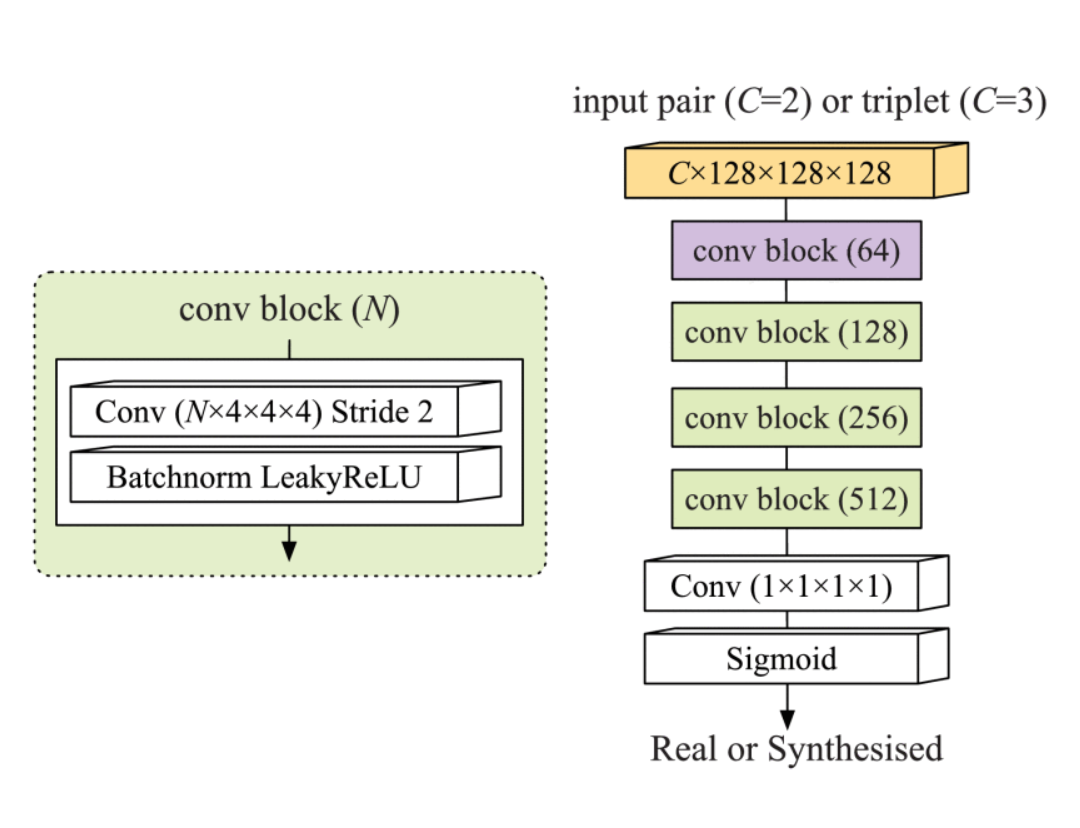
\includegraphics[width=0.7\textwidth]{Images/PIX2PIX-EAGAN DISCRIMINATOR.png}
    \caption{The 3D PatchGAN Discriminator architecture (reproduced from \cite{yu2019}). Convolutional and LeakyReLU layers with a slope of $0.2$ are applied to all conv blocks. Instance normalization is not used in the first block.}
    \label{fig:PIX-EAGAN D}
\end{figure}

\subsubsection{Objective Function}
The objective of a Conditional GAN is to learn a mapping from an observed image $x$ and a random noise vector $z$, to an output image $y$, denoted as $G: \{x, z\} \rightarrow y$. The objective function of the conditional GAN can be expressed as:

\begin{equation}
\mathcal{L}_{cGAN}(G, D) = \mathbb{E}_{x, y}[\log D(x, y)] + \mathbb{E}_{x, z}[\log(1 - D(x, G(x, z)))]
\end{equation}

where the Generator $G$ attempts to minimize this objective against an adversarial Discriminator $D$ that attempts to maximize it.

While the cGAN loss forces the generated images to look realistic and follow the distribution of the target domain, it does not strictly enforce structural similarity to the specific ground truth output $y$. To address this, a traditional regression loss is added to the Generator's objective. Pix2Pix utilizes the $L1$ distance instead of $L2$, as the $L1$ norm encourages less blurring and preserves sharper edges:

\begin{equation}
    \mathcal{L}_{L1}(G) = \mathbb{E}_{x, y, z}\left[||y - G(x, z)||_1\right]
\end{equation}

The total objective function is formulated as a combination of the conditional adversarial loss and the $L1$ loss, balanced by a weighting hyperparameter $\lambda$:

\begin{equation}
    G^* = \arg\min_G \max_D \mathcal{L}_{cGAN}(G, D) + \lambda \mathcal{L}_{L1}(G)
\end{equation}

By combining these two loss functions, the Pix2Pix framework leverages the PatchGAN (via $\mathcal{L}_{cGAN}$) to handle high-frequency details and the $L1$ loss to enforce low-frequency correctness, resulting in highly realistic and structurally coherent image translations.

\subsection{Ea-GAN}

While traditional Conditional GANs (such as Pix2Pix) focus primarily on voxel-wise intensity similarity for intra-modal synthesis, they often neglect the structural content and textural details of the images, leading to overly smoothed or blurry results. To address this limitation, Yu et al. (2019) \cite{yu2019} proposed Edge-Aware Generative Adversarial Networks for intra-modal Magnetic Resonance (MR) image synthesis. 

The original paper proposes two distinct frameworks: the Generator-Induced Ea-GAN (gEa-GAN), where edge constraints are applied solely as a penalty to the generator, and the Discriminator-Induced Ea-GAN (dEa-GAN), where edge maps are integrated into both the generator and the discriminator. Experimental evaluations demonstrate that the dEa-GAN is the most performant variant, as it allows structural edge preservation to be adversarially learned rather than just heavily penalized. For this reason, we selected the dEa-GAN architecture for our experiments. For the sake of clarity, hereafter in this thesis, we will refer to this chosen dEa-GAN model simply as \textbf{Ea-GAN}.

\subsubsection{Architecture and Edge Detection}

To extract structural details, the model utilizes a 3D Sobel edge detector, denoted as $S$. Three 3D Sobel filters ($F_i, F_j, F_k$), illustrated in Figure~\ref{fig:SOBEL}, are convolved with an input volume $A$ to extract intensity gradients along the three spatial directions. These gradients are then merged into a final edge map $S(A)$ according to the following equation:

\begin{figure}[htbp]
    \centering
    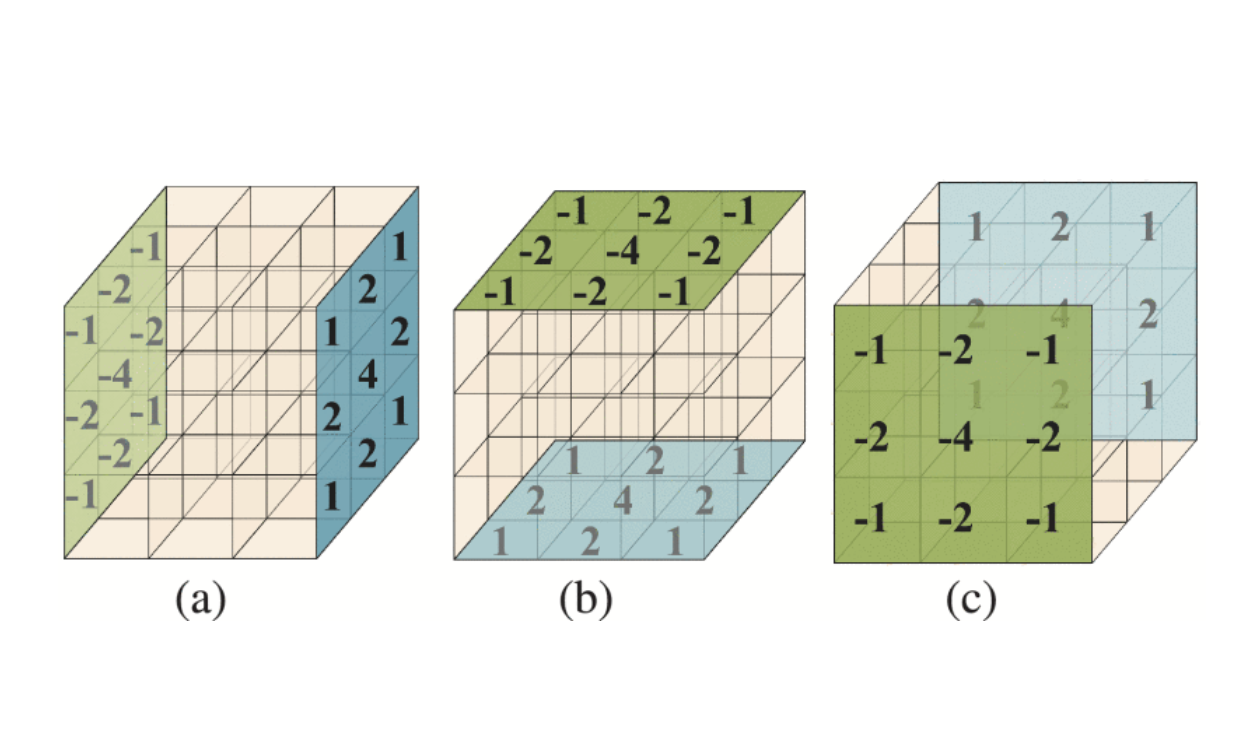
\includegraphics[width=0.6\textwidth]{Images/EAGAN_SOBEL.png}
    \caption{The three-dimensional Sobel operator includes three kernels as (a) $F_i$, (b) $F_j$, and (c) $F_k$, respectively (reproduced from \cite{yu2019}). The size of each kernel is $3 \times 3 \times 3$. Each empty cube without any number on its surface indicates a value of zero in the corresponding position of the kernel, whereas the numbers in the blue or green cubes represent the positive and negative values of the three kernels.}
    \label{fig:SOBEL}
\end{figure}

\begin{equation}
    S(A) = \sqrt{(F_i * A)^2 + (F_j * A)^2 + (F_k * A)^2}
\end{equation}
where $*$ denotes the convolution operation.

The generator component ($G$) shares the same 3D U-Net architecture described for Pix2Pix (Figure~\ref{fig:unet_pix2pix}). However, unlike the standard Pix2Pix generator that takes a single-channel 3D volume as input, the Ea-GAN generator takes a $2$-channel input, concatenating the source volume with its corresponding 3D edge map.

Likewise, the Pix2Pix discriminator evaluates a $2$-channel input (concatenated source and target/synthesized volumes), whereas the Ea-GAN discriminator evaluates a $3$-channel input: the source image, the target or synthesized image, and the corresponding target or synthesized edge map.

To extract these 3D edge maps dynamically during training, Ea-GAN incorporates a custom, differentiable 3D Sobel layer operating directly on the GPU. It applies three fixed $3 \times 3 \times 3$ convolutional kernels to compute spatial gradients along the axial, coronal, and sagittal axes. To prevent artificial gradients at the volume boundaries, the input is explicitly padded with a constant value of $-1.0$. The gradient magnitudes are aggregated using the $L2$ norm across the directional channels and passed through a \texttt{Tanh} activation function, safely scaling the edge maps to the $[-1, 1]$ range.



\begin{figure}[htbp]
    \centering
    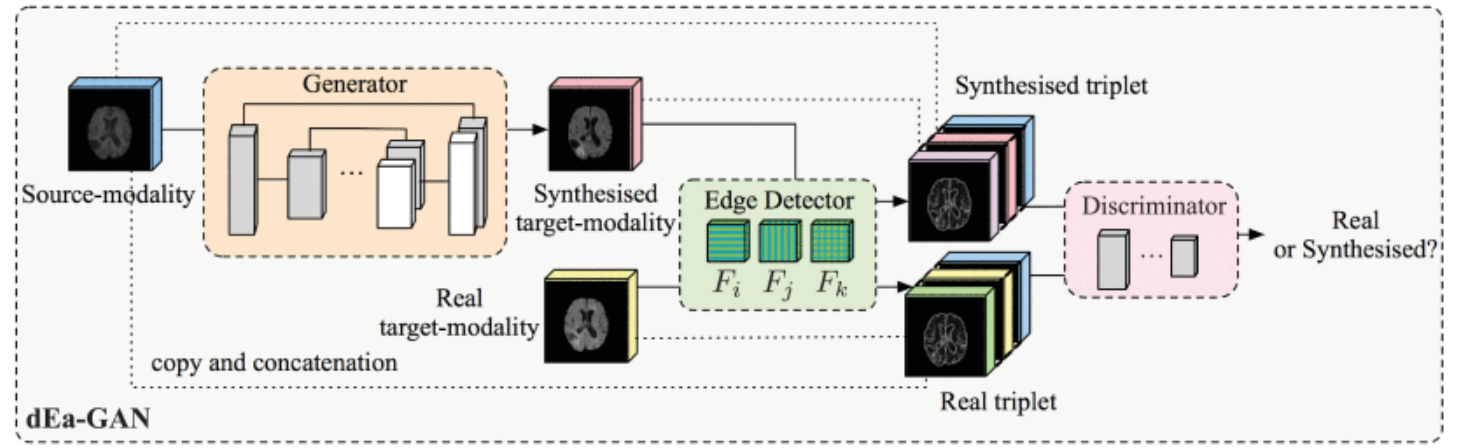
\includegraphics[width=0.9\textwidth]{Images/DEA-GAN.png}
    \caption{Overview of the chosen Ea-GAN (dEa-GAN) framework (reproduced from \cite{yu2019}). The edge map extracted by the Sobel operator $S$ is fed to both the generator and the discriminator, forcing the edge preservation to be adversarially learned.}
    \label{fig:eagan_framework}
\end{figure}

\subsubsection{Adversarial Learning Framework}
As mentioned, the chosen Ea-GAN fully exploits the min-max adversarial mechanism by integrating the edge maps into both the generator and the discriminator. 

In this configuration (Figure~\ref{fig:eagan_framework}), the discriminator $D$ is designed to evaluate a triplet instead of a simple image pair. It takes $(x, y, S(y))$ as real data, and $(x, G(x), S(G(x)))$ as synthesized data. By providing the discriminator with the edge maps, it learns to utilize fine edge details to differentiate between real and fake images. This dynamically forces the generator $G$ to produce highly accurate and sharp structural edges to fool the discriminator.

In addition to the adversarial loss, the generator is penalized by a voxel-wise $L1$ intensity loss and an $L1$ edge difference loss. The objective function for the generator is defined as:

\begin{equation}
\begin{split}
    \mathcal{L}_{Ea-GAN}^{G} &= \mathbb{E}_{x \sim p_{data}(x)}[\log(1 - D(x, G(x), S(G(x))))] \\
    &+ \lambda_{l1}\mathbb{E}_{x, y \sim p_{data}(x,y)}[\lVert y - G(x) \rVert_1] \\
    &+ \lambda_{edge}\mathbb{E}_{x, y \sim p_{data}(x,y)}[\lVert S(y) - S(G(x)) \rVert_1]
\end{split}
\end{equation}

where $\lambda_{l1}$ and $\lambda_{edge}$ are hyperparameters used to balance the intensity similarity and the edge preservation. On the other hand, the discriminator is trained to maximize its ability to distinguish the real triplets from the fake ones by minimizing the following cost function:

\begin{equation}
\begin{split}
    \mathcal{L}_{Ea-GAN}^{D} &= -\mathbb{E}_{x, y \sim p_{data}(x,y)}[\log D(x, y, S(y))] \\
    &- \mathbb{E}_{x \sim p_{data}(x)}[\log(1 - D(x, G(x), S(G(x))))]
\end{split}
\end{equation}

The network is optimized in an alternating fashion by minimizing the respective loss functions: $\min_G \mathcal{L}_{Ea-GAN}^{G}$ and $\min_D \mathcal{L}_{Ea-GAN}^{D}$.

\subsection{Pyramid Transformer Network (PTNet3D)}

Under a different architectural perspective, Zhang et al. (2022) \cite{ptnet3d} proposed the 3D Pyramid Transformer Network (PTNet3D), a novel framework that leverages the self-attention mechanisms of Transformers and Performers rather than traditional convolutional layers.

\subsubsection{Architecture and Attention Mechanisms}
Also the PTNet3D model adopts a U-Net-like structure, but replaces standard convolutional layers with a PerFormer Encoder (PFE), a PerFormer Decoder (PFD), and a central Transformer Bottleneck. 

\paragraph{Transformer Bottleneck and Performer Blocks}
The core advantage of a Transformer is its ability to capture global dependencies through a full-rank self-attention mechanism:
\begin{equation}
    \text{Attention}(Q, K, V) = \text{softmax}\left(\frac{QK^T}{\sqrt{d_k}}\right)V
\end{equation}
where $Q, K, V$ are the query, key, and value matrices, and $d_k$ is the dimension of the keys. However, computing this full-rank attention yields a quadratic time and space complexity with respect to the sequence length $L$, making it computationally infeasible for high-resolution 3D medical image blocks. 

To resolve this, PTNet3D confines the standard Transformer blocks strictly to the \textit{bottleneck} layer, where the spatial resolution is at its lowest, while employing \textit{Performer} blocks along the higher-resolution encoding and decoding paths (as illustrated in Figure~\ref{fig:ptnet3d_blocks}, reproduced from \cite{ptnet3d}). The Performer approximates the full-rank softmax attention via the Fast Attention Via positive Orthogonal Random features (FAVOR+) mechanism. By linearly approximating the softmax kernel, the Performer reduces the computational complexity from quadratic to linear:
\begin{equation}
    \widehat{\text{Attention}}(Q, K, V) = \hat{D}^{-1}\left(Q'((K')^T V)\right), \quad \hat{D} = \text{diag}(Q'(K')^T \mathbf{1}_L)
\end{equation}
where $Q'$ and $K'$ are the transformed queries and keys, which allow the order of matrix multiplication to be altered, thus saving significant computational resources.

\begin{figure}[htbp]
    \centering
    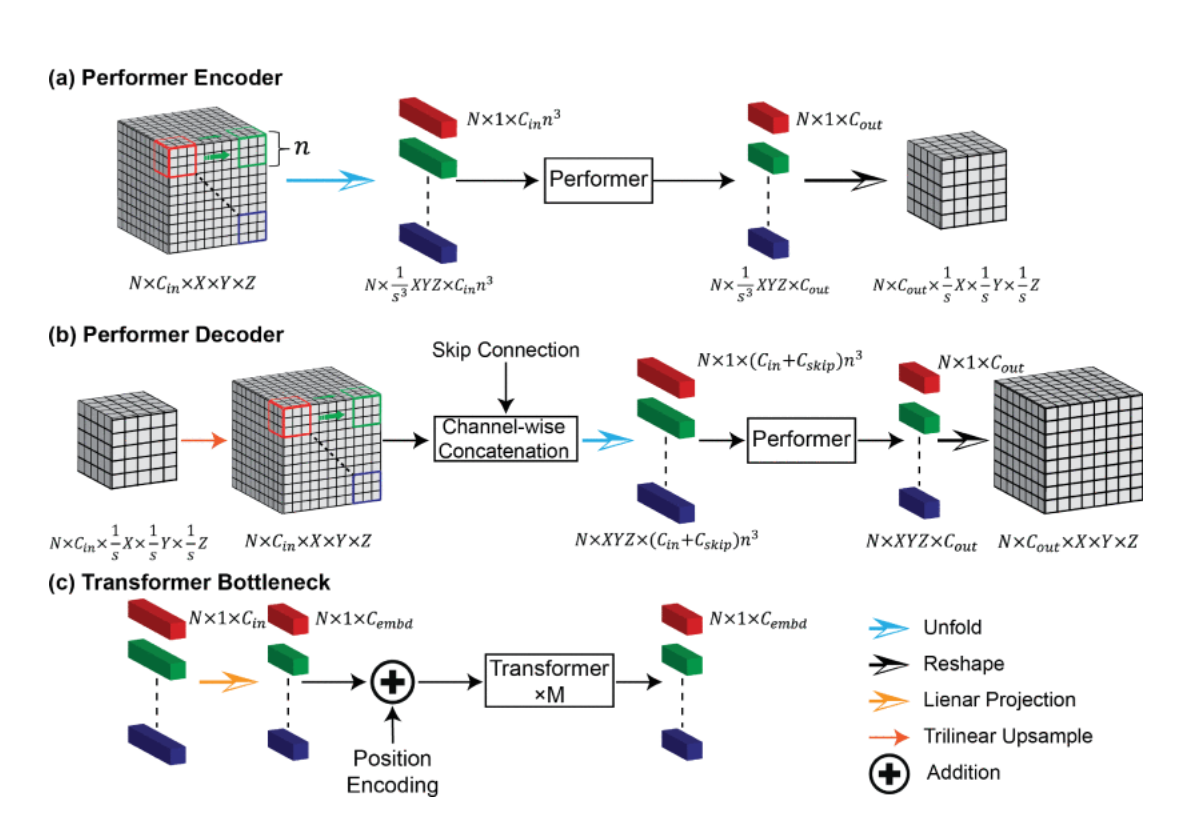
\includegraphics[width=0.5\textwidth]{Images/PERFORMER.png}
    \caption{Detailed structures of the Performer Encoder, Performer Decoder, and the Transformer Bottleneck in PTNet3D (reproduced from \cite{ptnet3d}). Performers are used in high-resolution paths, while full-rank Transformers are reserved for the bottleneck.}
    \label{fig:ptnet3d_blocks}
\end{figure}

\paragraph{Pyramid Representation}
Although the Performer significantly reduces computational costs, its mathematical approximation can lead to a potential loss of global contextual information compared to a full-rank Transformer. To compensate for this limitation, PTNet3D introduces a multi-scale \textit{pyramid layer} (schematically illustrated in Figure~\ref{fig:ptnet3d_overview}). The input volume is downsampled and fed into a parallel branch that relies solely on full-rank Transformer blocks. The feature maps from this pyramid branch are then concatenated back into the main network prior to the bottleneck, ensuring that global dependencies are accurately captured at multiple resolutions without exceeding memory limits.

\begin{figure}[htbp]
    \centering
    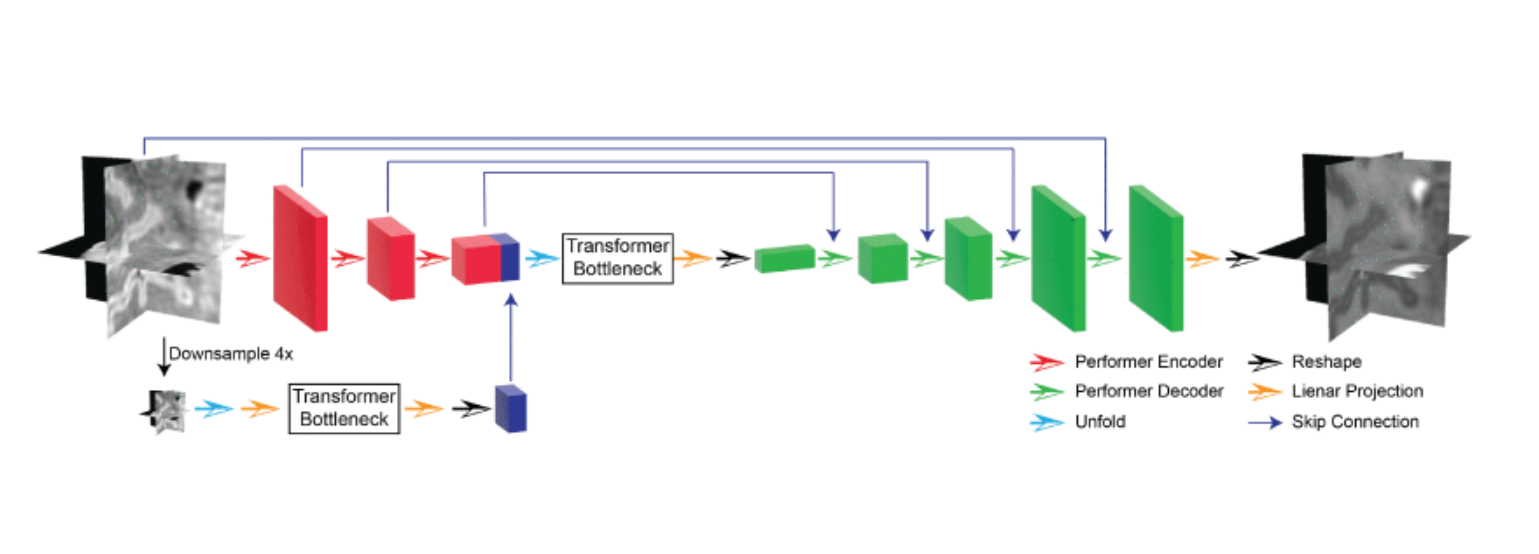
\includegraphics[width=0.9\textwidth]{Images/PTNET_ARCH.png}
    \caption{Overview of the 3D Pyramid Transformer Net (PTNet3D) architecture (reproduced from \cite{ptnet3d}). The model features a parallel pyramid representation that compensates for the information loss introduced by the Performer approximation.}
    \label{fig:ptnet3d_overview}
\end{figure}

\subsubsection{Adversarial Learning and Objective Function}
PTNet3D is trained within a GAN framework using a MultiscaleDiscriminator3D. This discriminator evaluates the concatenated $2$-channel input (the source volume and the target or synthesized volume) at $3$ different spatial scales simultaneously. At each scale, the discriminator processes the input through a sequence of 3D Convolutions utilizing $4 \times 4 \times 4$ kernels, escalating the feature maps from $64$ up to $256$. Each convolutional block, except the first and the last, is followed by 3D Instance Normalization and a LeakyReLU ($0.2$) activation function. To transition between the scales and progressively halve the spatial resolution, the network applies 3D Average Pooling with a kernel size of $3$, a stride of $2$, and a padding of $1$.

Unlike the previous CNN-based models, that rely heavily on the $L1$ norm for image reconstruction, ablation studies on PTNet3D demonstrated that optimal synthesis is achieved using a combination of four distinct losses:
\begin{itemize}
    \item \textbf{Voxel-wise MSE} ($\mathcal{L}_{MSE}$): To ensure basic structural fidelity and absolute intensity restoration.
    \item \textbf{Adversarial GAN Loss} ($\mathcal{L}_{adv}$): To encourage realistic global textures across all spatial scales.
    \item \textbf{Discriminator Feature Matching Loss} ($\mathcal{L}_{FM}$): To stabilize training by matching the intermediate representations extracted by the multiscale discriminator.
    \item \textbf{External Perceptual Loss} ($\mathcal{L}_{Perc}$): To preserve high-level semantic features, calculated by passing the real and synthesized volumes through a pre-trained 3D ResNet-18 utilized as an external feature extractor.
\end{itemize}

The total objective function for the PTNet3D generator is defined as:

\begin{equation}
    \mathcal{L}_{PTNet} = \mathcal{L}_{adv} + 10 \cdot \mathcal{L}_{FM} + 10 \cdot \mathcal{L}_{Perc} + 100 \cdot \mathcal{L}_{MSE}
\end{equation}

To mitigate the vanishing gradient problem typical of standard GANs, the adversarial loss $\mathcal{L}_{adv}$ is implemented using the Least Squares GAN (LSGAN) formulation. Specifically, the generator attempts to minimize the squared distance between the discriminator's output and the target label of real images (which is $1$):

\begin{equation}
    \mathcal{L}_{adv} = \mathbb{E}_{X}\left[\lVert D(X, G(X)) - 1 \rVert_2^2\right]
\end{equation}

Conversely, the discriminator is trained to minimize its own objective $\mathcal{L}_{D}$, classifying real images as $1$ and fake images as $0$:

\begin{equation}
    \mathcal{L}_{D} = \frac{1}{2} \mathbb{E}_{X,Y}\left[\lVert D(X, Y) - 1 \rVert_2^2\right] + \frac{1}{2} \mathbb{E}_{X}\left[\lVert D(X, G(X)) \rVert_2^2\right]
\end{equation}

The MSE loss $\mathcal{L}_{MSE}$ (for a source input $X$ and a target image $Y$) is formulated as:

\begin{equation}
    \mathcal{L}_{MSE} = \mathbb{E}_{X,Y}\left[\lVert G(X) - Y \rVert_2^2\right]
\end{equation}

Furthermore, the Discriminator Feature Matching loss $\mathcal{L}_{FM}$ computes the $L1$ distance between the intermediate feature maps of the real and synthesized images across the $S=3$ spatial scales of the discriminator:

\begin{equation}
    \mathcal{L}_{FM} = \mathbb{E}_{X,Y}\left[\sum_{i=1}^{S} \frac{1}{S} \sum_{j=1}^{L_i-1} \lVert D_{i}^{(j)}(X, Y) - D_{i}^{(j)}(X, G(X)) \rVert_1\right]
\end{equation}

where $L_i$ denotes the number of layers in the $i$-th discriminator scale, and $D_{i}^{(j)}$ represents the feature map extracted at the $j$-th layer of the $i$-th scale. Finally, the External Perceptual Loss $\mathcal{L}_{Perc}$ is mathematically defined as the $L1$ distance between the spatial activations extracted from the pre-trained 3D ResNet-18:

\begin{equation}
    \mathcal{L}_{Perc} = \mathbb{E}_{X,Y}\left[\sum_{l} \lambda_l \lVert \Phi_l(Y) - \Phi_l(G(X)) \rVert_1\right]
\end{equation}

where $\Phi_l$ denotes the feature map at the $l$-th extracted layer of the network, and $\lambda_l$ represents its corresponding scaling weight.

%-----------------------------------------------------------------------------
% CHAPTER 5
%-----------------------------------------------------------------------------

\section{Experimental setup}
\label{sec: 5}

\subsection{Implementation details}


All experiments, including the training, validation, and evaluation of the deep learning models presented in this work, were implemented and executed on the Kaggle cloud computing platform. To manage the substantial computational requirements and memory constraints associated with processing high-resolution 3D medical volumes and training complex 3D Generative Adversarial Networks, all procedures were accelerated utilizing a single NVIDIA Tesla T4 GPU equipped with 16 GB of dedicated VRAM. The core deep learning architectures were developed using the PyTorch framework, while the \texttt{TorchIO} library was primarily employed to handle the loading, spatial transformations, and patch-based extraction of the neuroimaging data.

\paragraph{Dataset Pairing and Cohort Selection}
Because the evaluated architectures (Pix2Pix, Ea-GAN, and PTNet3D) operate within a supervised image-to-image translation framework, their training strictly requires paired source and target volumetric scans. Consequently, we cross-referenced unique subject identifiers across the available cohorts to isolate the exact subsets of patients possessing both target sequences. As summarized in Table~\ref{tab:mri_matches}, these paired cohorts establish the precise voxel-wise correspondence required to compute the reconstruction, edge, and adversarial loss functions during training.

\begin{table}[H]
\centering
\small
\begin{tblr}{
  colspec = {lcc},
  hlines, vlines,
  row{1} = {font=\bfseries, c, m}
}
Modality 1 & Modality 2 & Paired Subjects (Matches) \\
T1         & FLAIR      & 1279 \\
T1         & T2         & 403 \\
T2         & FLAIR      & 399 \\
\end{tblr}
\vspace{1mm}
\centering
\caption{Exact number of matching unique subjects across the different structural MRI modalities (T1, T2, and FLAIR). These intersecting cohorts constitute the paired datasets used to train the translation models.}
\label{tab:mri_matches}
\end{table}

\subsubsection{3D Pix2Pix and Ea-GAN}

The original Pix2Pix model is natively designed as a 2D image-to-image translation network. However, to establish a fair and robust baseline for volumetric medical data, the authors of the Ea-GAN paper proposed a fully 3D extension of Pix2Pix, which we adopt in this work. Both models share a nearly identical core architecture---detailed in Section~\ref{sec: 4}---with Ea-GAN introducing specific modifications to dynamically process structural edge information.

\paragraph{Network Parameters}
Both the 3D Pix2Pix and Ea-GAN architectures optimize roughly $178.3$ million fully trainable parameters entirely from scratch. The vast majority of these reside in the shared 3D U-Net generator, which comprises $167{,}264{,}641$ parameters. Because the two models are structurally similar, their parameter counts diverge exclusively in the very first layer of the discriminator. The standard Pix2Pix PatchGAN discriminator (processing a 2-channel input) contains $11{,}033{,}025$ parameters. Conversely, the Ea-GAN discriminator evaluates a 3-channel input to simultaneously incorporate the additional structural edge maps. This minor architectural adaptation requires exactly $4{,}096$ additional weights in the initial 3D convolutional layer, bringing the total parameter count of the Ea-GAN discriminator to $11{,}037{,}121$.

\paragraph{Training and Optimization Details}

Both networks share the same initialization and training protocols. All convolutional weights are initialized from a Gaussian distribution with a mean of $0.0$ and a standard deviation of $0.02$. Instance Normalization weights are initialized with a mean of $1.0$ and a standard deviation of $0.02$.

Due to the massive memory footprint required to optimize the ${\sim}178$ million parameters of the 3D U-Net and 3D PatchGAN—which compute up to $512$ feature maps at their bottlenecks—passing an entire full-resolution MRI volume through the networks would immediately exceed the 16 GB capacity of the available NVIDIA T4 GPU. To overcome this hardware limitation, both models were trained using a patch-based strategy.

During the training phase, paired 3D sub-volumes (patches) of size $128 \times 128 \times 128$ voxels are randomly cropped on-the-fly from the original source and target scans. These paired patches are then stacked into mini-batches and fed into the networks. This localized sampling approach not only ensures an efficient memory allocation but also inherently acts as a robust form of spatial data augmentation. By observing different random sub-regions at each iteration, the models are forced to learn translation rules and fine-grained structural mappings that generalize across varying anatomical contexts. 

As explicitly prescribed by the authors in the original Ea-GAN paper, the networks were trained for a total of $150$ epochs: the optimizer's learning rate was kept fixed for the first $100$ epochs, and then linearly decayed to zero over the remaining $50$ epochs. In terms of computational cost, both models exhibited virtually identical execution times. Specifically, completing the full training schedule required approximately $75$ hours for the T1$\leftrightarrow$FLAIR transformations, whereas the T1$\leftrightarrow$T2 and T2$\leftrightarrow$FLAIR transformations required only about $25$ hours, a reduction directly proportional to the smaller number of available paired samples involving the T2 modality in the training dataset.

\subsubsection{PTNet3D}

The PTNet3D model introduces a fundamentally different architectural paradigm compared to standard convolutional models, relying on Transformers and Performers as detailed in Section~\ref{sec: 4}.

\paragraph{Network Parameters and VRAM Allocation}
To successfully execute this composite adversarial training, three distinct models must reside constantly in the GPU VRAM: the generator, the multiscale discriminator, and the external perceptual feature extractor. However, to keep the optimization process computationally tractable and preserve the learned representations in the pre-trained modules, only a specific subset of these parameters is actively updated during the backward pass. 

As detailed in Table~\ref{tab:ptnet_params}, while the discriminator parameters are fully trainable, the external pre-trained 3D ResNet utilized for the feature loss computation remains strictly frozen. Furthermore, the initial layers of the generator's internal encoder are explicitly excluded from the gradient computation. Consequently, of the approximately $49.12$ million total parameters loaded into the GPU memory, only $15.54$ million ($31.6\%$) are actively optimized. The remaining $68.4\%$ function exclusively as fixed computational graphs, a structural design that preserves pre-trained anatomical features while significantly mitigating the overall VRAM footprint.

\begin{table}[H]
\centering
\small
\begin{tblr}{
  colspec = {lccc},
  hlines, vlines,
  row{1} = {font=\bfseries, c, m}
}
Model Component & Total Params & Trainable Params & Frozen Params  \\
PTNet (Generator) & 8,013,257 & 7,598,025  & 415,232   \\
Discriminator & 7,939,395 & 7,939,395  & 0   \\
Ext. Extractor & 33,166,272 & 0  & 33,166,272  \\
\hline
\textbf{Total Training} & \textbf{49,118,924} & \textbf{15,537,420 (31.6\%)} & \textbf{33,581,504 (68.4\%)} \\
\end{tblr}
\vspace{1mm}
\caption{Distribution of network parameters during the training phase of PTNet3D. All three components reside in VRAM simultaneously, but the external feature extractor and the early layers of the generator's encoder are frozen to optimize memory usage and preserve pre-trained weights.}
\label{tab:ptnet_params}
\end{table}

\paragraph{Training and Optimization Details}
To accommodate the heavy memory footprint dictated by the attention mechanisms, the multiscale discrimination, and the auxiliary 3D ResNet feature extractor outlined above, the model processes the volumetric data using a patch-based strategy. During training, paired 3D sub-volumes (patches) of size $64 \times 64 \times 64$ voxels are randomly cropped on-the-fly from the full-resolution source and target MR volumes. These extracted patches are then stacked into mini-batches of size $4$ and fed to the network. By optimizing the model on these localized regions rather than on entire scans simultaneously, the network can learn fine-grained mappings and complex local textures while strictly maintaining a manageable GPU memory allocation. 

Regarding the training duration, the authors of the original PTNet3D paper recommend determining the total number of epochs based on the dataset size, following the heuristic rule: \(\text{Total Epochs} \approx 500,000 \, / \, N\), where \(N\) is the total number of volumetric scans available for training. Typically, this computed total is divided equally between a phase with a fixed learning rate and a subsequent phase with a linearly decaying learning rate. In strict accordance with this iterative rule, the total number of training epochs was dynamically calculated based on the available paired samples in each dataset. Consequently, the network was trained for $386$ epochs for the T1$\leftrightarrow$FLAIR transformations, and for $1240$ epochs for the T1$\leftrightarrow$T2 and T2$\leftrightarrow$FLAIR transformations. The network parameters were updated using the Adam optimizer with an initial learning rate of $0.0002$. Following standard optimization practices for this architecture, the learning rate was maintained constant for the first half of the total training epochs, and subsequently linearly decayed to zero over the remaining half. In strict accordance with the simplified random sampling strategy provided by the original authors---which extracts exactly one volumetric patch per scan per epoch---this methodology fixes the absolute number of sampled patches processed by the network to exactly $500,000$ for all modalities. Given our mini-batch size of $4$, this precisely corresponds to $125,000$ forward-backward network iterations, ensuring that the computational training time remained perfectly constant (requiring approximately $84$ hours per task) regardless of the underlying dataset size.

\subsubsection*{Voxel-level and statistical metrics}
\noindent
\textbf{Mean Absolute Error (MAE):} The Mean Absolute Error \cite{willmott2005advantages} measures the average magnitude of absolute pixel-level differences between the synthesized and ground truth images. Unlike Mean Squared Error (MSE), MAE provides a direct, linear quantification of synthesis error without excessively penalizing outliers. A lower MAE score indicates a better voxel-wise intensity agreement. The metric is defined as:
\begin{align}
    \text{MAE}(x, y) = \frac{1}{N} \sum_{i=1}^{N} |x_i - y_i|
\end{align}
where $N$ is the total number of voxels, and $x_i$ and $y_i$ represent the intensity values of the $i$-th voxel in the synthesized image $x$ and the ground truth image $y$, respectively. A value closer to $0$ is targeted for MAE, with typical values falling in the $[0, 1]$ range.

\vspace{2mm}
\noindent
\textbf{Peak Signal-to-Noise Ratio (PSNR):} To assess absolute intensity restoration, we utilize the Peak Signal-to-Noise Ratio (PSNR) \cite{wang2009mean, huynh2008scope}, which measures the ratio between the maximum possible signal and the mean squared error (MSE) noise. While PSNR provides a standard benchmark for image quality, it remains highly sensitive to global brightness differences. It is calculated as:
\begin{align}
    \text{PSNR}(x, y) = 20 \log_{10} \left( \frac{MAX_I}{\sqrt{\text{MSE}(x,y)}} \right)
\end{align}
where $MAX_I$ denotes the maximum possible pixel intensity of the image. The PSNR is measured in dB, with values ideally ranging between 25 and 40.

\vspace{2mm}
\noindent
\textbf{Normalized Cross-Correlation (NCC):} To account for the limitations of PSNR, we supplement the evaluation with the Normalized Cross-Correlation (NCC) \cite{lewis1995fast, maintz1998survey}. NCC measures the linear correlation of intensities and is invariant to linear intensity transformations (such as global brightness and contrast shifts), making it highly reliable for cross-modal and multi-scanner MRI evaluation. The NCC is computed as:
\begin{align}
    \text{NCC}(x, y) = \frac{\sum (x - \bar{x})(y - \bar{y})}{\sqrt{\sum (x - \bar{x})^2 \sum (y - \bar{y})^2}}
\end{align}
where $\bar{x}$ and $\bar{y}$ denote the mean intensities of images $x$ and $y$. The NCC values fall in the $[-1, 1]$ range, with a target score of $> 0.85$.

\subsubsection*{Structural and perceptual fidelity metrics}
\noindent
\textbf{Structural Similarity Index Measure (SSIM):} The SSIM index \cite{wang2004image} evaluates the similarity between two images by jointly considering three distinct perceptual components: luminance, contrast, and structure. Unlike purely pixel-wise metrics, SSIM captures distortions that are perceptually meaningful to the human visual system. The index is derived from the combination of three independent comparison functions applied to local image windows $x$ and $y$:
\begin{itemize}
    \item \textbf{Luminance ($l$):} Estimated using the mean intensities $\mu_x$ and $\mu_y$, it compares the global brightness of the two windows: $l(x, y) = \frac{2\mu_x\mu_y + C_1}{\mu_x^2 + \mu_y^2 + C_1}$.
    \item \textbf{Contrast ($c$):} Estimated using the standard deviations $\sigma_x$ and $\sigma_y$, it evaluates the difference in intensity variance: $c(x, y) = \frac{2\sigma_x\sigma_y + C_2}{\sigma_x^2 + \sigma_y^2 + C_2}$.
    \item \textbf{Structure ($s$):} Computed using the covariance $\sigma_{xy}$, it measures the correlation of the local structural patterns after normalizing for luminance and contrast: $s(x, y) = \frac{\sigma_{xy} + C_3}{\sigma_x\sigma_y + C_3}$.
\end{itemize}
By setting $C_3 = C_2 / 2$ and combining these components via multiplication ($SSIM = l \cdot c \cdot s$), the simplified mathematical definition of the global SSIM is given as follows:
\begin{align}
    \text{SSIM}(x, y) = \frac{(2\mu_x\mu_y + C_1)(2\sigma_{xy} + C_2)}{(\mu_x^2 + \mu_y^2 + C_1)(\sigma_x^2 + \sigma_y^2 + C_2)}
\end{align}
where $C_1$ and $C_2$ are small constants added for numerical stability to prevent division by zero. A higher SSIM score indicates greater overall similarity between the synthesized and ground-truth images, with values falling in the $[-1, 1]$ range and a typical target $> 0.85$.

\vspace{2mm}
\noindent
\textbf{Feature Similarity Index Measure (FSIM):} The Feature Similarity Index Measure (FSIM) \cite{zhang2011fsim} evaluates similarity based on human visual system mechanisms, heavily relying on two critical low-level features: Phase Congruency (PC) and Gradient Magnitude (GM). 
\begin{itemize}
    \item \textbf{Phase Congruency (PC):} This is a dimensionless quantity that identifies highly significant local structures (such as edges and corners) based on the frequency domain, specifically where the Fourier components are maximally in phase. As implemented, it is extracted using banks of \textbf{log-Gabor filters}. By computing the 2D Fast Fourier Transform (FFT) and extracting the even and odd filter responses, the local amplitude and phase energy are determined. Because PC is mathematically invariant to variations in image brightness and contrast, it acts as a highly robust primary feature.
    \item \textbf{Gradient Magnitude (GM):} While PC is contrast-independent, GM is explicitly computed to capture the absolute strength of local contrast and edge variations. In this implementation, GM is calculated using the \textbf{Scharr gradient operator}. The image is convolved with horizontal and vertical Scharr kernels to obtain directional gradients $G_x$ and $G_y$, and the magnitude is derived as $\sqrt{G_x^2 + G_y^2}$.
\end{itemize}
For any two images $x$ and $y$, local similarity maps $S_{PC}(x,y)$ and $S_{GM}(x,y)$ are independently computed for these two features. These similarity maps evaluate the pointwise alignment between the features using a normalized correlation formula, mathematically defined as:
\begin{align}
    S_{PC}(x, y) &= \frac{2 \cdot PC(x) \cdot PC(y) + C_1}{PC(x)^2 + PC(y)^2 + C_1} \\
    S_{GM}(x, y) &= \frac{2 \cdot GM(x) \cdot GM(y) + C_2}{GM(x)^2 + GM(y)^2 + C_2}
\end{align}
where $C_1$ and $C_2$ are positive constants included to increase numerical stability. 
The final FSIM score aggregates these pointwise similarities, using the maximum phase congruency $PC_m = \max(PC(x), PC(y))$ as a spatial weighting function to assign greater importance to regions with prominent structural features. The global formula is expressed as:
\begin{align}
    \text{FSIM}(x, y) = \frac{\sum \big[S_{PC}(x,y) \cdot S_{GM}(x,y) \cdot PC_m\big]}{\sum PC_m}
\end{align}
where a higher FSIM value indicates a superior preservation of anatomical contours, local sharpness, and global feature coherence. The metric ranges from $0$ to $1$, with a typical target $> 0.85$.

\vspace{2mm}
\noindent
\textbf{Learned Perceptual Image Patch Similarity (LPIPS):} The Learned Perceptual Image Patch Similarity (LPIPS) metric \cite{zhang2018unreasonable} measures perceptual similarity between two images by comparing feature activations from a deep neural network, making it sensitive to semantic and textural differences and aligned with human visual perception. A lower LPIPS score indicates higher similarity. In this work, we utilized the \textbf{AlexNet} architecture, comprising $2{,}470{,}848$ parameters, as the backbone feature extractor. 

Since LPIPS is natively defined for RGB 2D images, the comparison is performed by extracting 2D slices from the MRI volumes and converting them to RGB by replicating the single grayscale channel across the three color channels. The LPIPS formula is given by:
\begin{align}
\text{LPIPS}(x, y) = \sum_l \frac{1}{H_l W_l} \sum_{h,w} \| w_l \big( f^l(x)_{hw} - f^l(y)_{hw} \big) \|^2
\end{align}
where \( f^l(x) \) and \( f^l(y) \) are the deep features at layer \( l \) for images \( x \) and \( y \), \( w_l \) are the learned weights, and \( H_l \) and \( W_l \) denote the height and width of the feature map at layer \( l \). LPIPS values are strictly positive, with a target score of $< 0.20$.

\subsection{Evaluation}

\paragraph{Test Datasets Pairing}
Similarly to the training phase, the quantitative evaluation of the synthesized volumes strictly requires perfectly paired ground-truth reference scans to compute the quality metrics (e.g., LPIPS, SSIM, and PSNR). For the internal test split of the ADNI cohort, we applied the same cross-referencing procedure used for the training set, identifying the exact intersections of patients who possessed both required modalities. 

Furthermore, to robustly evaluate the generalization capabilities of our models on different scanners, field strengths, and patient populations, we integrated the two additional external test sets introduced in Section~\ref{subsec:datasets}: the IXI dataset for the T1$\leftrightarrow$T2 translation task, and the OpenNeuro dataset for the T1$\leftrightarrow$FLAIR translation task. The resulting paired matches reserved for the testing and evaluation phase across all three datasets are summarized in Table~\ref{tab:test_mri_matches}.

\begin{table}[H]
\centering
\small
\begin{tblr}{
  colspec = {llcc},
  hlines, vlines,
  row{1} = {font=\bfseries, c, m},
  cell{2}{1} = {c, m} % Centra verticalmente il testo "ADNI"
}
Dataset & Modality 1 & Modality 2 & Paired Subjects (Matches) \\
\SetCell[r=3]{} ADNI & T1 & FLAIR & 221 \\
                      & T1 & T2    & 89 \\
                      & T2 & FLAIR & 87 \\
IXI                   & T1 & T2    & 577 \\
OpenNeuro             & T1 & FLAIR & 170 \\
\end{tblr}
\vspace{1mm}
\caption{Exact number of matching paired subjects across the structural MRI modalities in the test datasets. These paired subsets were utilized as ground-truth references to systematically compute the evaluation metrics for the image-to-image translation models.}
\label{tab:test_mri_matches}
\end{table}

\paragraph{Patch-Based Volumetric Inference}
Consistent with the strategy adopted during the training phase, processing entire high-resolution 3D MRI volumes in a single forward pass remained computationally prohibitive during testing due to substantial GPU memory (VRAM) constraints. To circumvent these hardware limitations during the evaluation phase, we similarly opted for a patch-based approach. However, to systematically reconstruct the complete synthesized volumes without losing spatial context, the inference was executed in a sliding-window manner.

Specifically, each complete input 3D volume was systematically divided into overlapping 3D sub-volumes (patches) using a \texttt{GridSampler}. To ensure consistency and maximize the effectiveness of the learned representations, we strictly maintained the native patch sizes on which each model was originally trained. For the fully convolutional models (3D Pix2Pix and Ea-GAN), we utilized their native patch size of $128 \times 128 \times 128$ voxels with a spatial overlap of $64 \times 64 \times 64$ voxels. Conversely, for the transformer-based PTNet3D architecture inference was performed using its native $64 \times 64 \times 64$ voxel patch size with a proportional spatial overlap.

Each extracted patch is independently processed by the Generator model to synthesize the corresponding target modality patch. Subsequently, the full synthetic MRI volume is seamlessly reconstructed using a \texttt{GridAggregator}. To prevent the formation of visible grid-like seams and artifacts at the boundaries of adjacent patches, the aggregator employs an averaging overlap scheme, which smoothly interpolates the overlapping predicted intensities. Finally, all quantitative evaluation metrics are rigorously computed directly on these fully reconstructed macroscopic volumes, ensuring a holistic assessment of the generated anatomical structures rather than isolated patches.

\subsubsection{Downstream Tasks}
To rigorously assess the clinical utility and anatomical fidelity of the synthesized MRI volumes beyond standard pixel-wise and perceptual metrics, we evaluated their performance on two distinct, clinically relevant downstream tasks: brain age estimation (a complex regression task) and epilepsy classification (a challenging binary classification task). These downstream applications serve as an excellent proxy to determine whether the generative models successfully preserved biologically and pathologically meaningful structural details.

\paragraph{Task 1: Brain Age Estimation}
Brain age prediction is highly sensitive to minute morphological changes in the brain. For this task, we employed the Simple Fully Convolutional Network (SFCN) architecture \cite{PENG2021101871}, a lightweight and highly effective 3D CNN explicitly designed for this purpose. The evaluation was conducted on the external IXI dataset, which naturally exhibits significant domain variance as its data was acquired across three distinct clinical sites in London: Guy's Hospital (Guys), Hammersmith Hospital (HH), and the Institute of Psychiatry (IOP). It is important to note that out of the entire IXI cohort, demographic age metadata was only available for a subset of $545$ unique patients, which therefore constitutes the final dataset utilized for this specific task. Specifically, this cohort comprises $301$ subjects from Guys, $177$ from HH, and $67$ from IOP. The chronological age distribution of this final subset is visualized in Figure~\ref{fig:ixi_age_dist}.

\begin{figure}[H]
    \centering
    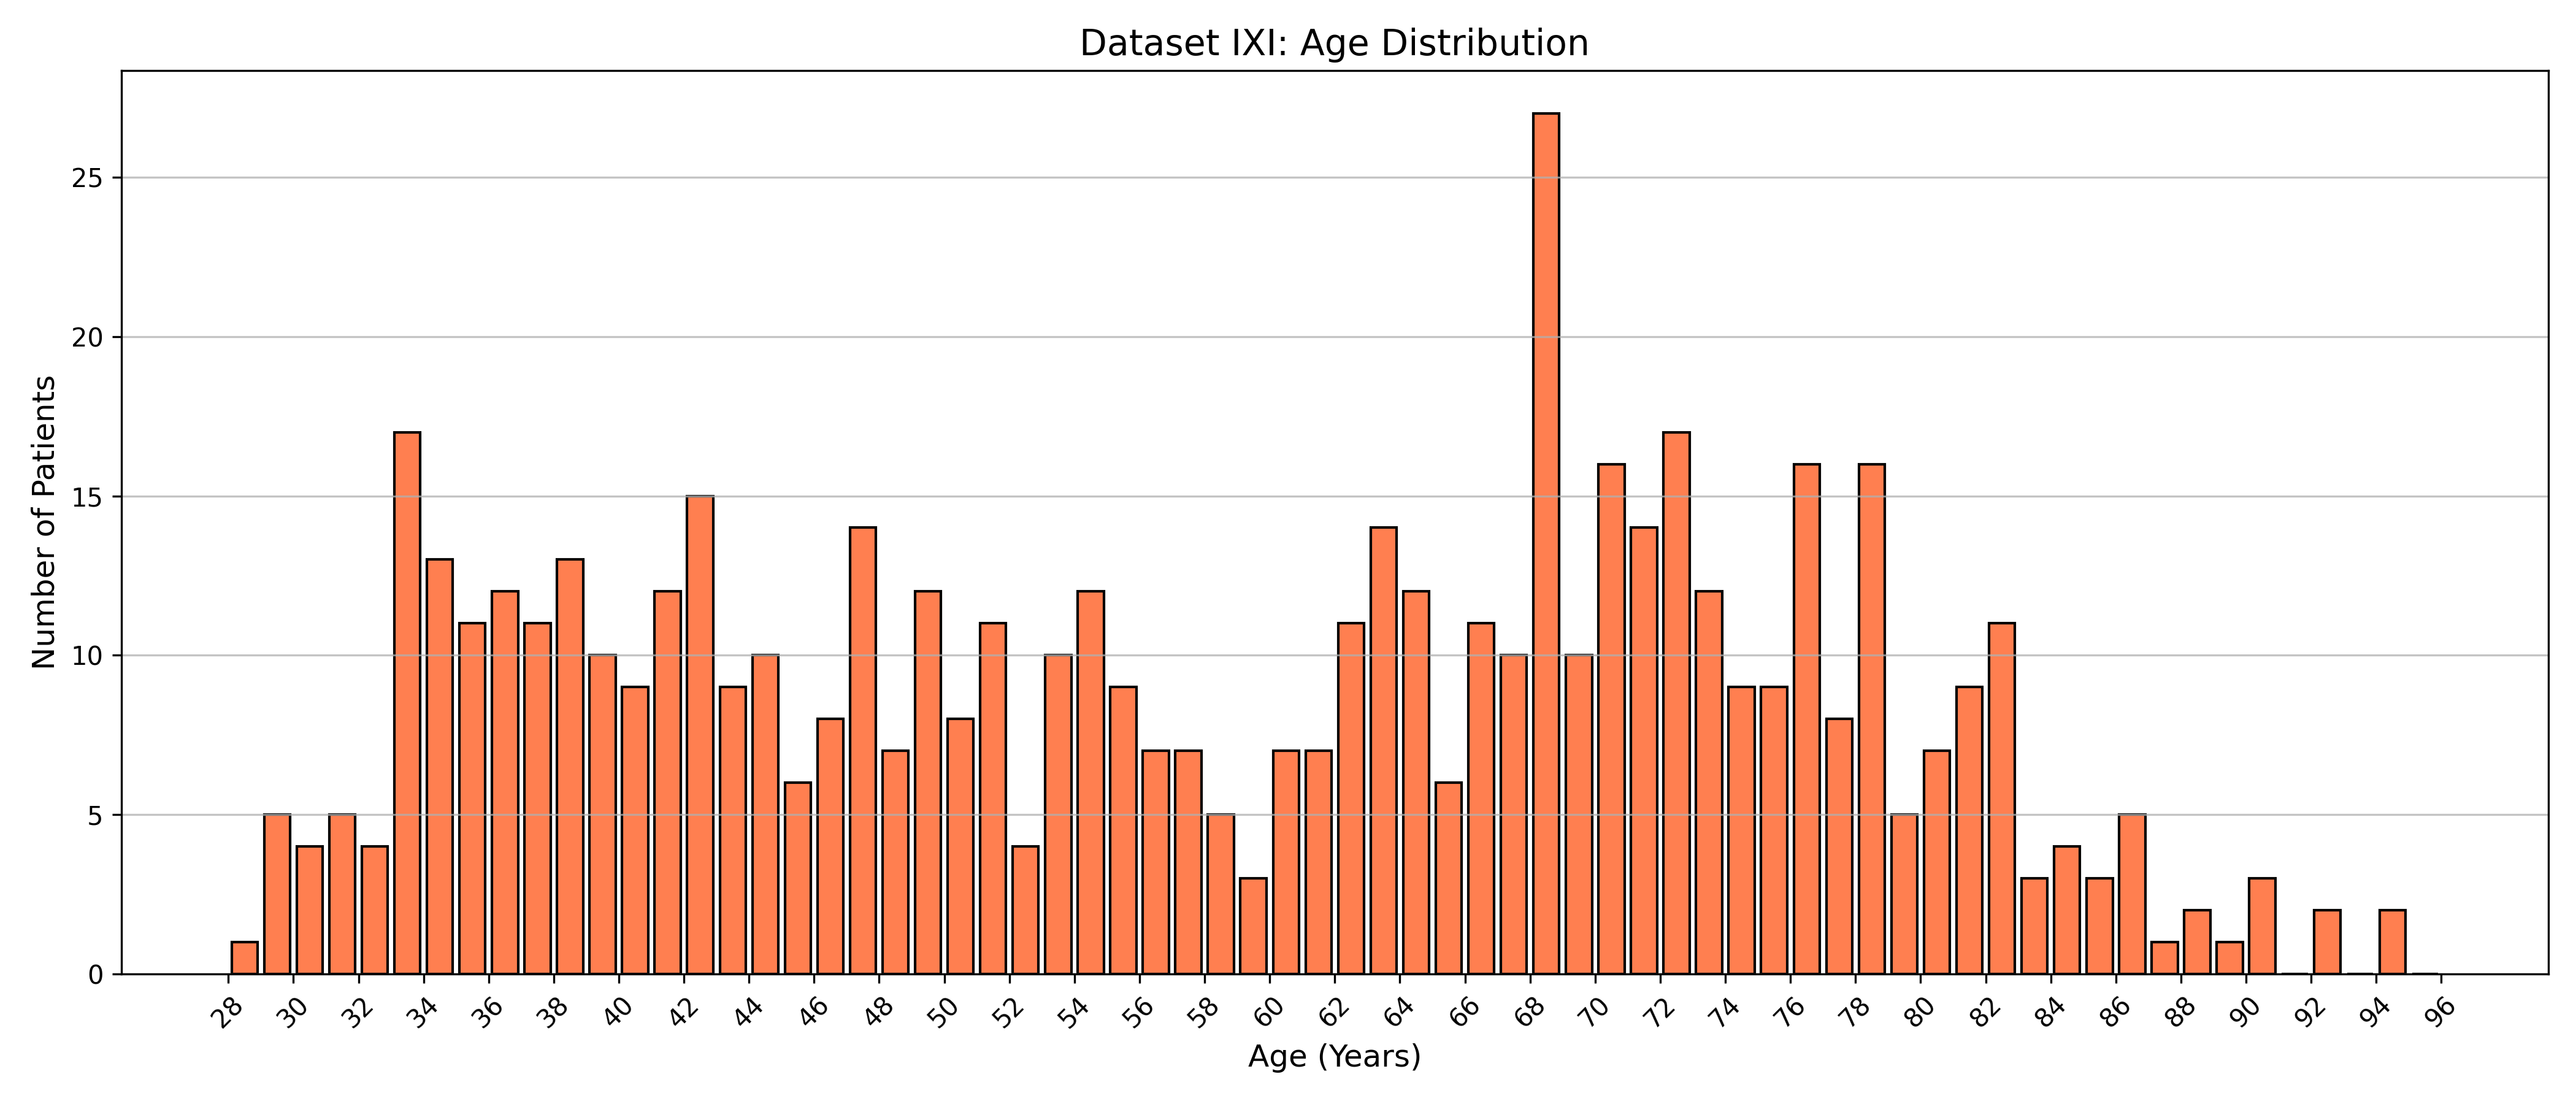
\includegraphics[width=0.75\textwidth]{Images/IXI age distr.png}
    \caption{Chronological age distribution of the $545$ subjects in the IXI dataset utilized for the downstream brain age estimation task.}
    \label{fig:ixi_age_dist}
\end{figure}

To simultaneously evaluate the synthetic data quality and cross-domain generalization, we implemented a Leave-One-Site-Out Cross-Validation (LOSO-CV) strategy. In each fold of the cross-validation, the \textit{real} ground-truth MRIs from the left-out site were strictly reserved for validation. To comprehensively benchmark the downstream utility of the synthesized images, we conducted a comparative analysis by training the SFCN model from scratch under three distinct configurations using the data from the remaining two sites:
\begin{itemize}
    \item \textbf{Real-only (Baseline):} The network was trained exclusively on the real MRIs, establishing the upper-bound baseline performance of the model on authentic data.
    \item \textbf{Synthetic-only:} The network was trained exclusively on the synthetic MRIs generated by our models, testing their viability as a direct substitute for authentic data.
    \item \textbf{Hybrid (Data Augmentation):} The network was trained on a combined dataset comprising both real and synthetic MRIs, investigating the potential of our generative models to serve as an effective data augmentation strategy.
\end{itemize}

The downstream model employed is the Simple Fully Convolutional Network (SFCN), which consists of a VGG-style feature extractor followed by a classifier head, as illustrated in Figure~\ref{fig:sfcn_arch}. The feature extraction backbone is composed of five consecutive convolutional blocks, which progressively expand the feature channels as $\{32, 64, 128, 256, 256\}$. This is followed by a $1\times1\times1$ convolutional block reducing the channels to $64$. The classification head applies a global 3D Average Pooling over the remaining spatial dimensions ($5 \times 6 \times 5$), a Dropout layer ($p=0.5$), and a final $1\times1\times1$ convolution mapping the latent features to the output dimension. Crucially, rather than utilizing a fixed arbitrary number of output bins, we dynamically adapted the output channels of this final layer to precisely match the specific demographic age bounds of our dataset. 

\begin{figure}[H]
    \centering
    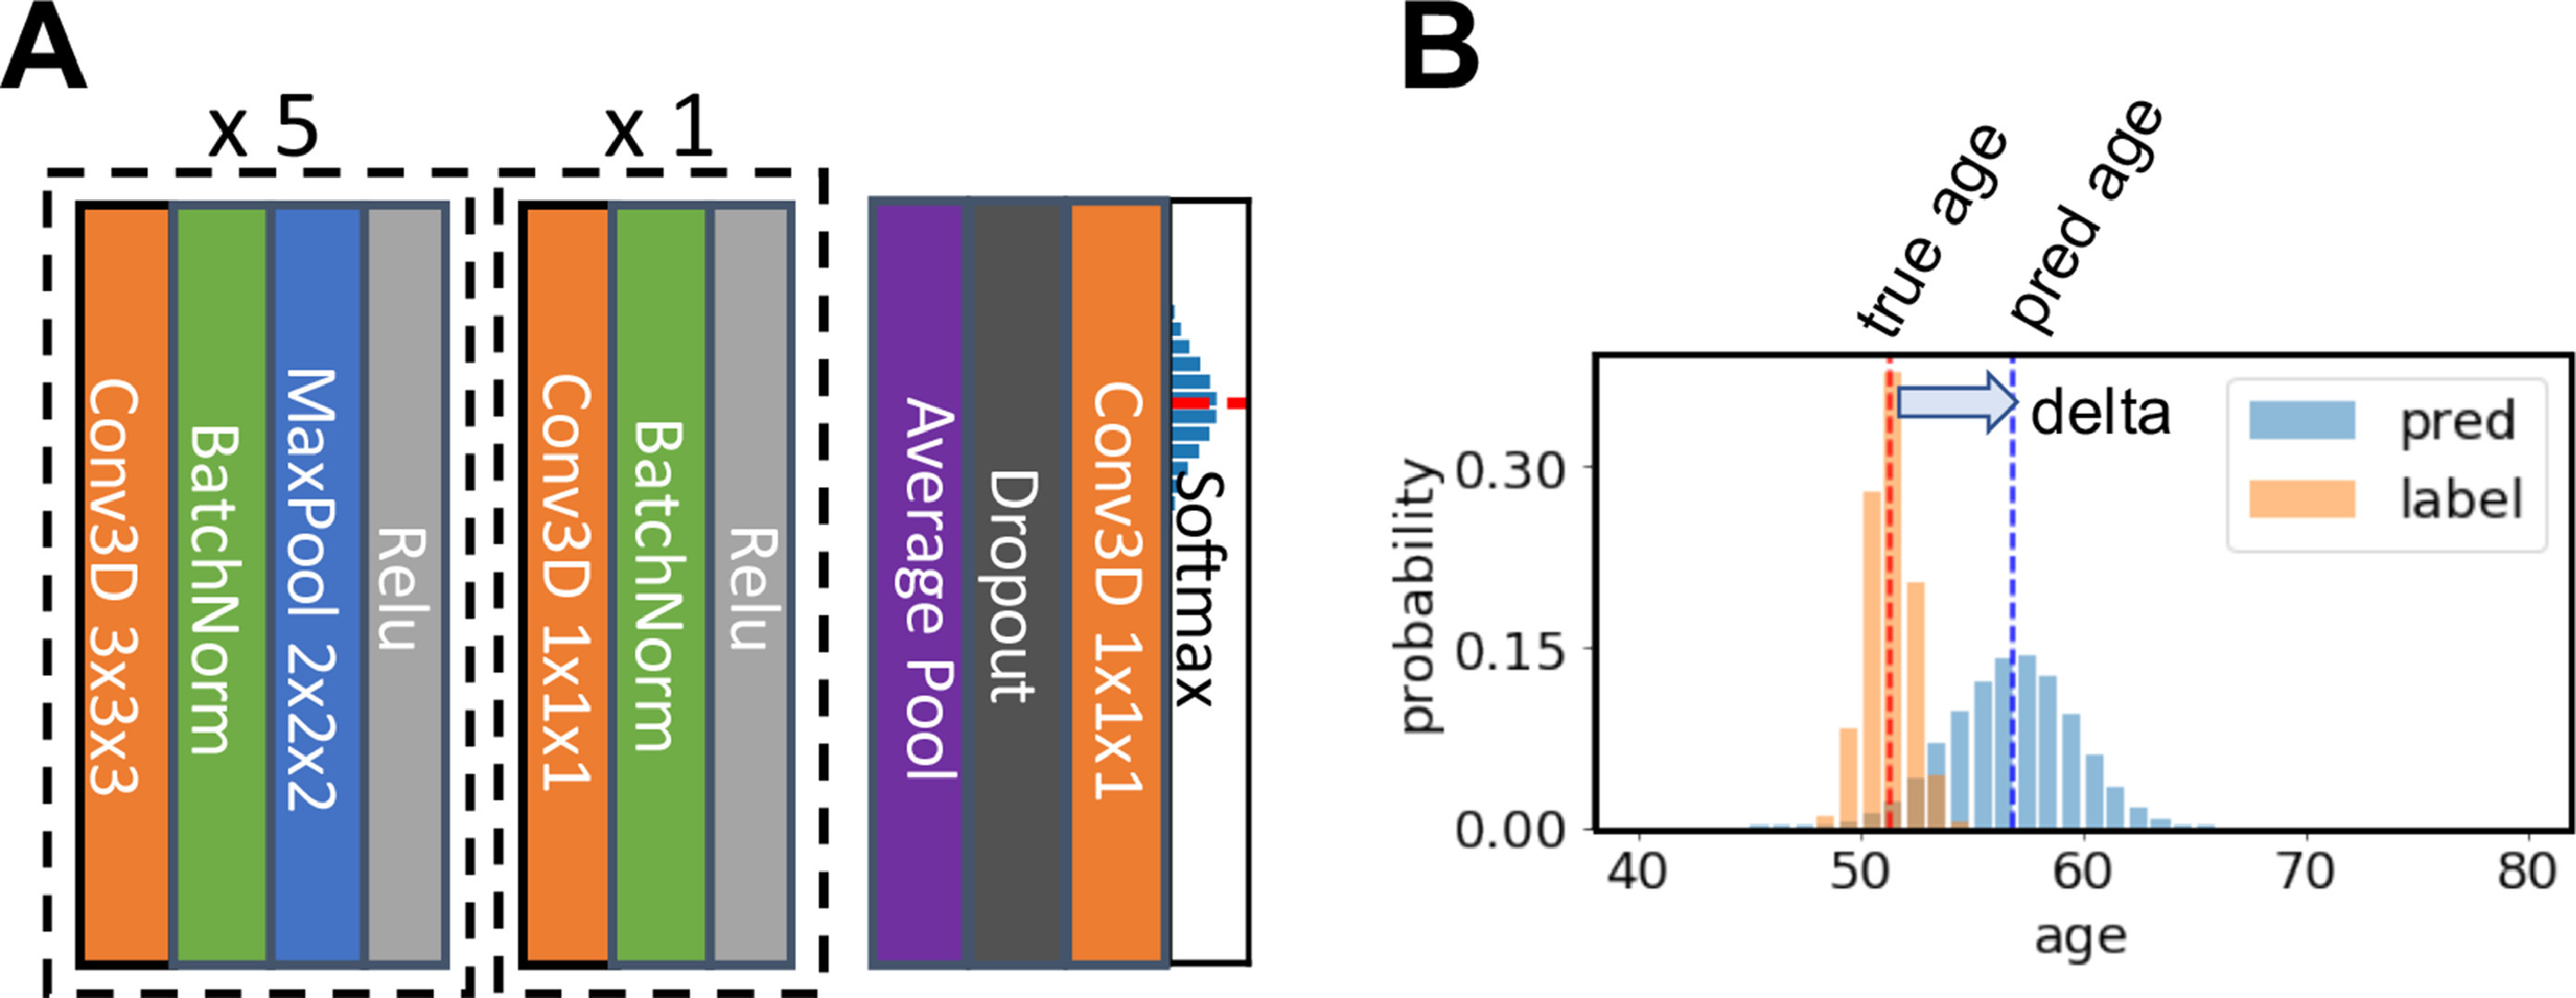
\includegraphics[width=0.9\textwidth]{Images/arch_SFCN.jpg}
    \caption{Overview of the Simple Fully Convolutional Network (SFCN) architecture employed for brain age prediction (reproduced from \cite{PENG2021101871}).}
    \label{fig:sfcn_arch}
\end{figure}

The SFCN model processes the 3D MRI volumes center-cropped to a standardized spatial resolution of $160 \times 192 \times 160$ voxels. Following the original SFCN methodology, the regression problem was formulated as a soft-classification task, predicting age probabilities across discrete 1-year age bins. Rather than employing standard one-hot encoding or mean squared error regression, the chronological age was represented using a label smoothing approach, projecting the true age into a discrete Gaussian distribution centered around the actual age value. 

To ensure a fair and methodologically sound comparison, the training hyperparameters were kept strictly identical across all three data configurations (Real, Synthetic, and Hybrid). Specifically, the network was trained from scratch for a maximum of $200$ epochs using a batch size of $8$. Optimization was performed using the Adam optimizer with a learning rate of $1 \times 10^{-4}$ and a weight decay of $1 \times 10^{-3}$. The loss function employed was the Kullback-Leibler (KL) Divergence, which effectively minimizes the statistical discrepancy between the predicted age probability distribution and the true age Gaussian distribution. An early stopping mechanism was implemented with a patience of $30$ epochs to reliably prevent overfitting on the validation set. The overall performance of the downstream task was finally quantified using the Mean Absolute Error (MAE) alongside the Pearson correlation coefficient ($r$).


\paragraph{Task 2: Epilepsy Classification (HC vs FCD)}
As a second downstream task, we evaluated the capability of the synthesized images to preserve subtle pathological features by formulating a binary classification problem: distinguishing between Healthy Controls (HC) and patients diagnosed with Focal Cortical Dysplasia (FCD). FCD is a localized malformation of cortical development and a highly common cause of medically intractable epilepsy, often presenting with very subtle structural abnormalities on MRI scans that are notoriously difficult to detect even by expert neuroradiologists.

For this classification task, we utilized the external OpenNeuro dataset (specifically targeting the FCD cohort). To adapt the SFCN architecture and prevent severe overfitting on this binary classification task, we reduced the number of feature channels in the convolutional backbone to $\{28, 58, 128, 256, 256, 64\}$—the identical configuration successfully utilized by the authors for their binary Male/Female sex classification task—and restricted the final classification output dimension strictly to $2$. 

Due to the more limited sample size of the FCD cohort, and given that the scans were acquired at a single clinical site---rendering a Leave-One-Site-Out (LOSO) cross-validation scheme inapplicable---we adopted a robust $5$-Fold Cross-Validation strategy to reliably assess model performance across the entire dataset. Notably, the cohort is perfectly balanced between healthy controls and diseased patients ($85$ subjects per class). Furthermore, the cross-validation splits were rigorously stratified, ensuring that the target class distribution within both the training and validation sets of every single fold remained strictly balanced. 

In each fold, the binary classifier was trained from scratch for a maximum of $150$ epochs with a batch size of $4$. The network was optimized using the Adam optimizer (learning rate $1 \times 10^{-4}$, weight decay $1 \times 10^{-3}$) and a standard Cross-Entropy loss function, combined with an early stopping patience of $25$ epochs. Similar to the age estimation task, we systematically evaluated the performance of the classifier trained purely on real images, and subsequently benchmarked it against models trained on generated images and hybrid data augmentation setups. The overall performance for this clinical task was comprehensively evaluated using the global Accuracy score and the Area Under the Receiver Operating Characteristic Curve (ROC-AUC).


%-----------------------------------------------------------------------------
% CHAPTER 6
%-----------------------------------------------------------------------------

\section{Results \& Discussion}
\label{sec: 6}

\subsection{Quantitative Results}

The quantitative evaluation of the synthesized MRI volumes is presented in Table~\ref{tab:results_t1_t2_full} for the T1$\leftrightarrow$T2 task, Table~\ref{tab:results_t1_flair_full} for the T1$\leftrightarrow$FLAIR task, and Table~\ref{tab:results_t2_flair} for the T2$\leftrightarrow$FLAIR task. The analysis is divided between the internal test set (ADNI) and the external, unseen datasets (IXI and OpenNeuro) to thoroughly assess both the pure synthesis quality and the out-of-distribution generalization capabilities of the proposed architectures.

\begin{table}[H]
\centering
\resizebox{\textwidth}{!}{%
\begin{tabular}{lllcccccc}
\hline\hline\noalign{\smallskip}
\textbf{Dataset} & \textbf{Direction} & \textbf{Model} & \textbf{MAE ($\downarrow$)} & \textbf{PSNR ($\uparrow$)} & \textbf{SSIM ($\uparrow$)} & \textbf{NCC ($\uparrow$)} & \textbf{LPIPS ($\downarrow$)} & \textbf{FSIM ($\uparrow$)} \\
\noalign{\smallskip}\hline\noalign{\smallskip}

% --- BLOCCO ADNI (Internal Test) ---
\multirow{6}{*}{ADNI} 
    & \multirow{3}{*}{T1 $\rightarrow$ T2} 
                & Pix2Pix & $0.058 \pm 0.009$ & $\mathbf{25.290 \pm 1.267}$ & $0.823 \pm 0.048$ & $0.943 \pm 0.013$ & $0.061 \pm 0.011$ & $0.898 \pm 0.018$ \\
    &           & Ea-GAN  & $\mathbf{0.053 \pm 0.009}$ & $24.789 \pm 1.642$ & $\mathbf{0.837 \pm 0.059}$ & $\mathbf{0.951 \pm 0.013}$ & $\mathbf{0.060 \pm 0.011}$ & $\mathbf{0.911 \pm 0.018}$ \\
    &           & PTNet3D & $0.087 \pm 0.020$ & $21.430 \pm 1.348$ & $0.819 \pm 0.063$ & $0.908 \pm 0.013$ & $0.078 \pm 0.015$ & $0.845 \pm 0.019$ \\
\cline{2-9}\noalign{\smallskip}
    & \multirow{3}{*}{T2 $\rightarrow$ T1} 
                & Pix2Pix & $\mathbf{0.051 \pm 0.010}$ & $24.540 \pm 1.936$ & $\mathbf{0.858 \pm 0.050}$ & $0.966 \pm 0.009$ & $0.046 \pm 0.011$ & $0.924 \pm 0.019$ \\
    &           & Ea-GAN  & $0.052 \pm 0.010$ & $\mathbf{24.749 \pm 2.005}$ & $0.856 \pm 0.047$ & $\mathbf{0.967 \pm 0.009}$ & $\mathbf{0.043 \pm 0.010}$ & $\mathbf{0.928 \pm 0.018}$ \\
    &           & PTNet3D & $0.105 \pm 0.017$ & $20.234 \pm 1.075$ & $0.829 \pm 0.050$ & $0.926 \pm 0.012$ & $0.077 \pm 0.010$ & $0.850 \pm 0.016$ \\
\hline\noalign{\smallskip}

% --- BLOCCO IXI (External Test) ---
\multirow{6}{*}{IXI} 
    & \multirow{3}{*}{T1 $\rightarrow$ T2} 
                & Pix2Pix & $\mathbf{0.101 \pm 0.017}$ & $\mathbf{21.836 \pm 1.494}$ & $0.679 \pm 0.075$ & $0.840 \pm 0.062$ & $0.147 \pm 0.033$ & $0.770 \pm 0.063$ \\
    &           & Ea-GAN  & $0.107 \pm 0.019$ & $21.218 \pm 1.658$ & $0.688 \pm 0.084$ & $\mathbf{0.849 \pm 0.065}$ & $\mathbf{0.107 \pm 0.034}$ & $\mathbf{0.780 \pm 0.071}$ \\
    &           & PTNet3D & $0.110 \pm 0.019$ & $19.680 \pm 1.356$ & $\mathbf{0.715 \pm 0.087}$ & $0.823 \pm 0.063$ & $0.124 \pm 0.032$ & $0.751 \pm 0.062$ \\
\cline{2-9}\noalign{\smallskip}
    & \multirow{3}{*}{T2 $\rightarrow$ T1} 
                & Pix2Pix & $\mathbf{0.100 \pm 0.024}$ & $\mathbf{20.940 \pm 1.995}$ & $0.743 \pm 0.076$ & $\mathbf{0.860 \pm 0.055}$ & $0.107 \pm 0.037$ & $0.801 \pm 0.069$ \\
    &           & Ea-GAN  & $0.103 \pm 0.026$ & $20.825 \pm 2.073$ & $0.731 \pm 0.079$ & $0.857 \pm 0.056$ & $\mathbf{0.105 \pm 0.038}$ & $\mathbf{0.802 \pm 0.072}$ \\
    &           & PTNet3D & $0.118 \pm 0.023$ & $19.253 \pm 1.428$ & $\mathbf{0.766 \pm 0.074}$ & $0.852 \pm 0.044$ & $0.129 \pm 0.034$ & $0.772 \pm 0.059$ \\
\hline\hline

\end{tabular}%
}
\vspace{2mm}
\caption{Quantitative evaluation of the \textbf{T1 $\leftrightarrow$ T2} translation task across the internal (ADNI) and external (IXI) test datasets. Results are reported as mean $\pm$ standard deviation. The best results for each metric and direction are highlighted in \textbf{bold}.}
\label{tab:results_t1_t2_full}
\end{table}


\begin{table}[H]
\centering
\resizebox{\textwidth}{!}{%
\begin{tabular}{lllcccccc}
\hline\hline\noalign{\smallskip}
\textbf{Dataset} & \textbf{Direction} & \textbf{Model} & \textbf{MAE ($\downarrow$)} & \textbf{PSNR ($\uparrow$)} & \textbf{SSIM ($\uparrow$)} & \textbf{NCC ($\uparrow$)} & \textbf{LPIPS ($\downarrow$)} & \textbf{FSIM ($\uparrow$)} \\
\noalign{\smallskip}\hline\noalign{\smallskip}

% --- BLOCCO ADNI (Internal Test) ---
\multirow{6}{*}{ADNI} 
    & \multirow{3}{*}{T1 $\rightarrow$ FLAIR} 
                & Pix2Pix & $0.060 \pm 0.018$ & $17.376 \pm 2.239$ & $0.586 \pm 0.152$ & $\mathbf{0.936 \pm 0.035}$ & $0.084 \pm 0.024$ & $0.883 \pm 0.027$ \\
    &           & Ea-GAN  & $\mathbf{0.059 \pm 0.017}$ & $\mathbf{18.588 \pm 2.299}$ & $\mathbf{0.636 \pm 0.148}$ & $0.934 \pm 0.035$ & $\mathbf{0.073 \pm 0.023}$ & $\mathbf{0.891 \pm 0.025}$ \\
    &           & PTNet3D & $0.142 \pm 0.032$ & $17.833 \pm 1.880$ & $0.577 \pm 0.129$ & $0.890 \pm 0.036$ & $0.127 \pm 0.034$ & $0.785 \pm 0.036$ \\
\cline{2-9}\noalign{\smallskip}
    & \multirow{3}{*}{FLAIR $\rightarrow$ T1} 
                & Pix2Pix & $0.053 \pm 0.011$ & $\mathbf{24.405 \pm 1.850}$ & $0.845 \pm 0.053$ & $0.954 \pm 0.024$ & $0.064 \pm 0.018$ & $0.908 \pm 0.022$ \\
    &           & Ea-GAN  & $\mathbf{0.052 \pm 0.010}$ & $24.237 \pm 1.692$ & $\mathbf{0.856 \pm 0.049}$ & $\mathbf{0.955 \pm 0.021}$ & $\mathbf{0.058 \pm 0.017}$ & $\mathbf{0.913 \pm 0.021}$ \\
    &           & PTNet3D & $0.103 \pm 0.019$ & $20.050 \pm 1.226$ & $0.792 \pm 0.066$ & $0.895 \pm 0.026$ & $0.097 \pm 0.020$ & $0.826 \pm 0.022$ \\
\hline\noalign{\smallskip}

% --- BLOCCO OPENNEURO (External Test) ---
\multirow{6}{*}{OpenNeuro} 
    & \multirow{3}{*}{T1 $\rightarrow$ FLAIR} 
                & Pix2Pix & $0.080 \pm 0.015$ & $\mathbf{16.204 \pm 1.197}$ & $0.617 \pm 0.069$ & $0.847 \pm 0.048$ & $0.139 \pm 0.022$ & $0.775 \pm 0.032$ \\
    &           & Ea-GAN  & $\mathbf{0.078 \pm 0.012}$ & $16.176 \pm 1.090$ & $\mathbf{0.627 \pm 0.065}$ & $0.841 \pm 0.052$ & $\mathbf{0.135 \pm 0.023}$ & $\mathbf{0.785 \pm 0.031}$ \\
    &           & PTNet3D & $0.181 \pm 0.020$ & $15.419 \pm 0.991$ & $0.590 \pm 0.074$ & $\mathbf{0.848 \pm 0.055}$ & $0.156 \pm 0.033$ & $0.776 \pm 0.026$ \\
\cline{2-9}\noalign{\smallskip}
    & \multirow{3}{*}{FLAIR $\rightarrow$ T1} 
                & Pix2Pix & $0.074 \pm 0.017$ & $\mathbf{24.500 \pm 2.017}$ & $0.830 \pm 0.080$ & $0.932 \pm 0.047$ & $\mathbf{0.067 \pm 0.047}$ & $\mathbf{0.897 \pm 0.044}$ \\
    &           & Ea-GAN  & $\mathbf{0.069 \pm 0.017}$ & $24.459 \pm 2.045$ & $\mathbf{0.848 \pm 0.082}$ & $\mathbf{0.936 \pm 0.044}$ & $0.072 \pm 0.046$ & $0.893 \pm 0.045$ \\
    &           & PTNet3D & $0.084 \pm 0.019$ & $21.464 \pm 1.321$ & $0.832 \pm 0.084$ & $0.896 \pm 0.033$ & $0.118 \pm 0.030$ & $0.805 \pm 0.031$ \\
\hline\hline

\end{tabular}%
}

\vspace{2mm}
\caption{Quantitative evaluation of the \textbf{T1 $\leftrightarrow$ FLAIR} translation task across the internal (ADNI) and external (OpenNeuro) test datasets. Results are reported as mean $\pm$ standard deviation. The best results for each metric and direction are highlighted in \textbf{bold}.}
\label{tab:results_t1_flair_full}
\end{table}

\begin{table}[H]
\centering
\resizebox{\textwidth}{!}{%
\begin{tabular}{lllcccccc}
\hline\hline\noalign{\smallskip}
\textbf{Dataset} & \textbf{Direction} & \textbf{Model} & \textbf{MAE ($\downarrow$)} & \textbf{PSNR ($\uparrow$)} & \textbf{SSIM ($\uparrow$)} & \textbf{NCC ($\uparrow$)} & \textbf{LPIPS ($\downarrow$)} & \textbf{FSIM ($\uparrow$)} \\
\noalign{\smallskip}\hline\noalign{\smallskip}

% --- BLOCCO ADNI ---
\multirow{6}{*}{ADNI} 
    & \multirow{3}{*}{T2 $\rightarrow$ FLAIR} 
                & Pix2Pix & $0.068 \pm 0.014$ & $\mathbf{22.826 \pm 1.935}$ & $\mathbf{0.785 \pm 0.054}$ & $0.950 \pm 0.020$ & $0.069 \pm 0.015$ & $0.878 \pm 0.015$ \\
    &           & Ea-GAN  & $\mathbf{0.062 \pm 0.014}$ & $20.397 \pm 2.274$ & $0.731 \pm 0.079$ & $\mathbf{0.956 \pm 0.019}$ & $\mathbf{0.062 \pm 0.015}$ & $\mathbf{0.895 \pm 0.017}$ \\
    &           & PTNet3D & $0.149 \pm 0.034$ & $17.344 \pm 1.628$ & $0.687 \pm 0.089$ & $0.926 \pm 0.018$ & $0.116 \pm 0.024$ & $0.798 \pm 0.027$ \\
\cline{2-9}\noalign{\smallskip}
    & \multirow{3}{*}{FLAIR $\rightarrow$ T2} 
                & Pix2Pix & $0.055 \pm 0.011$ & $24.922 \pm 1.467$ & $0.825 \pm 0.050$ & $0.949 \pm 0.016$ & $0.076 \pm 0.014$ & $0.887 \pm 0.022$ \\
    &           & Ea-GAN  & $\mathbf{0.054 \pm 0.011}$ & $\mathbf{25.276 \pm 1.489}$ & $\mathbf{0.827 \pm 0.047}$ & $\mathbf{0.951 \pm 0.015}$ & $\mathbf{0.068 \pm 0.012}$ & $\mathbf{0.896 \pm 0.019}$ \\
    &           & PTNet3D & $0.094 \pm 0.017$ & $21.270 \pm 1.419$ & $0.732 \pm 0.064$ & $0.895 \pm 0.023$ & $0.093 \pm 0.020$ & $0.834 \pm 0.024$ \\
\hline\hline

\end{tabular}%
}
\vspace{2mm}
\caption{Quantitative evaluation of the \textbf{T2 $\leftrightarrow$ FLAIR} translation task across the internal test dataset (ADNI). Results are reported as mean $\pm$ standard deviation. The best results for each metric and direction are highlighted in \textbf{bold}.}
\label{tab:results_t2_flair}
\end{table}

\subsection{Qualitative Results}

Visual inspection of the synthesized MRI volumes provides critical insights into the perceptual fidelity, anatomical preservation, and artifact generation of the evaluated models. To demonstrate the cross-domain generalization capabilities of our architectures, the qualitative samples for the T1$\leftrightarrow$T2 and T1$\leftrightarrow$FLAIR tasks are deliberately selected from the external test datasets (IXI and OpenNeuro, respectively). For the T2$\leftrightarrow$FLAIR task, where external datasets were unavailable, the samples are drawn from the internal ADNI test set.

\subsubsection*{T1 $\leftrightarrow$ T2 Translation (IXI Dataset)}
Figures \ref{fig:qual_t1_t2} and \ref{fig:qual_t2_t1} present comparative slices of the T1$\rightarrow$T2 and T2$\rightarrow$T1 translations on the unseen IXI dataset, respectively. The images contrast the ground-truth target scans with the synthesized outputs generated by Pix2Pix, Ea-GAN, and PTNet3D.

\begin{figure}[H]
    \centering
    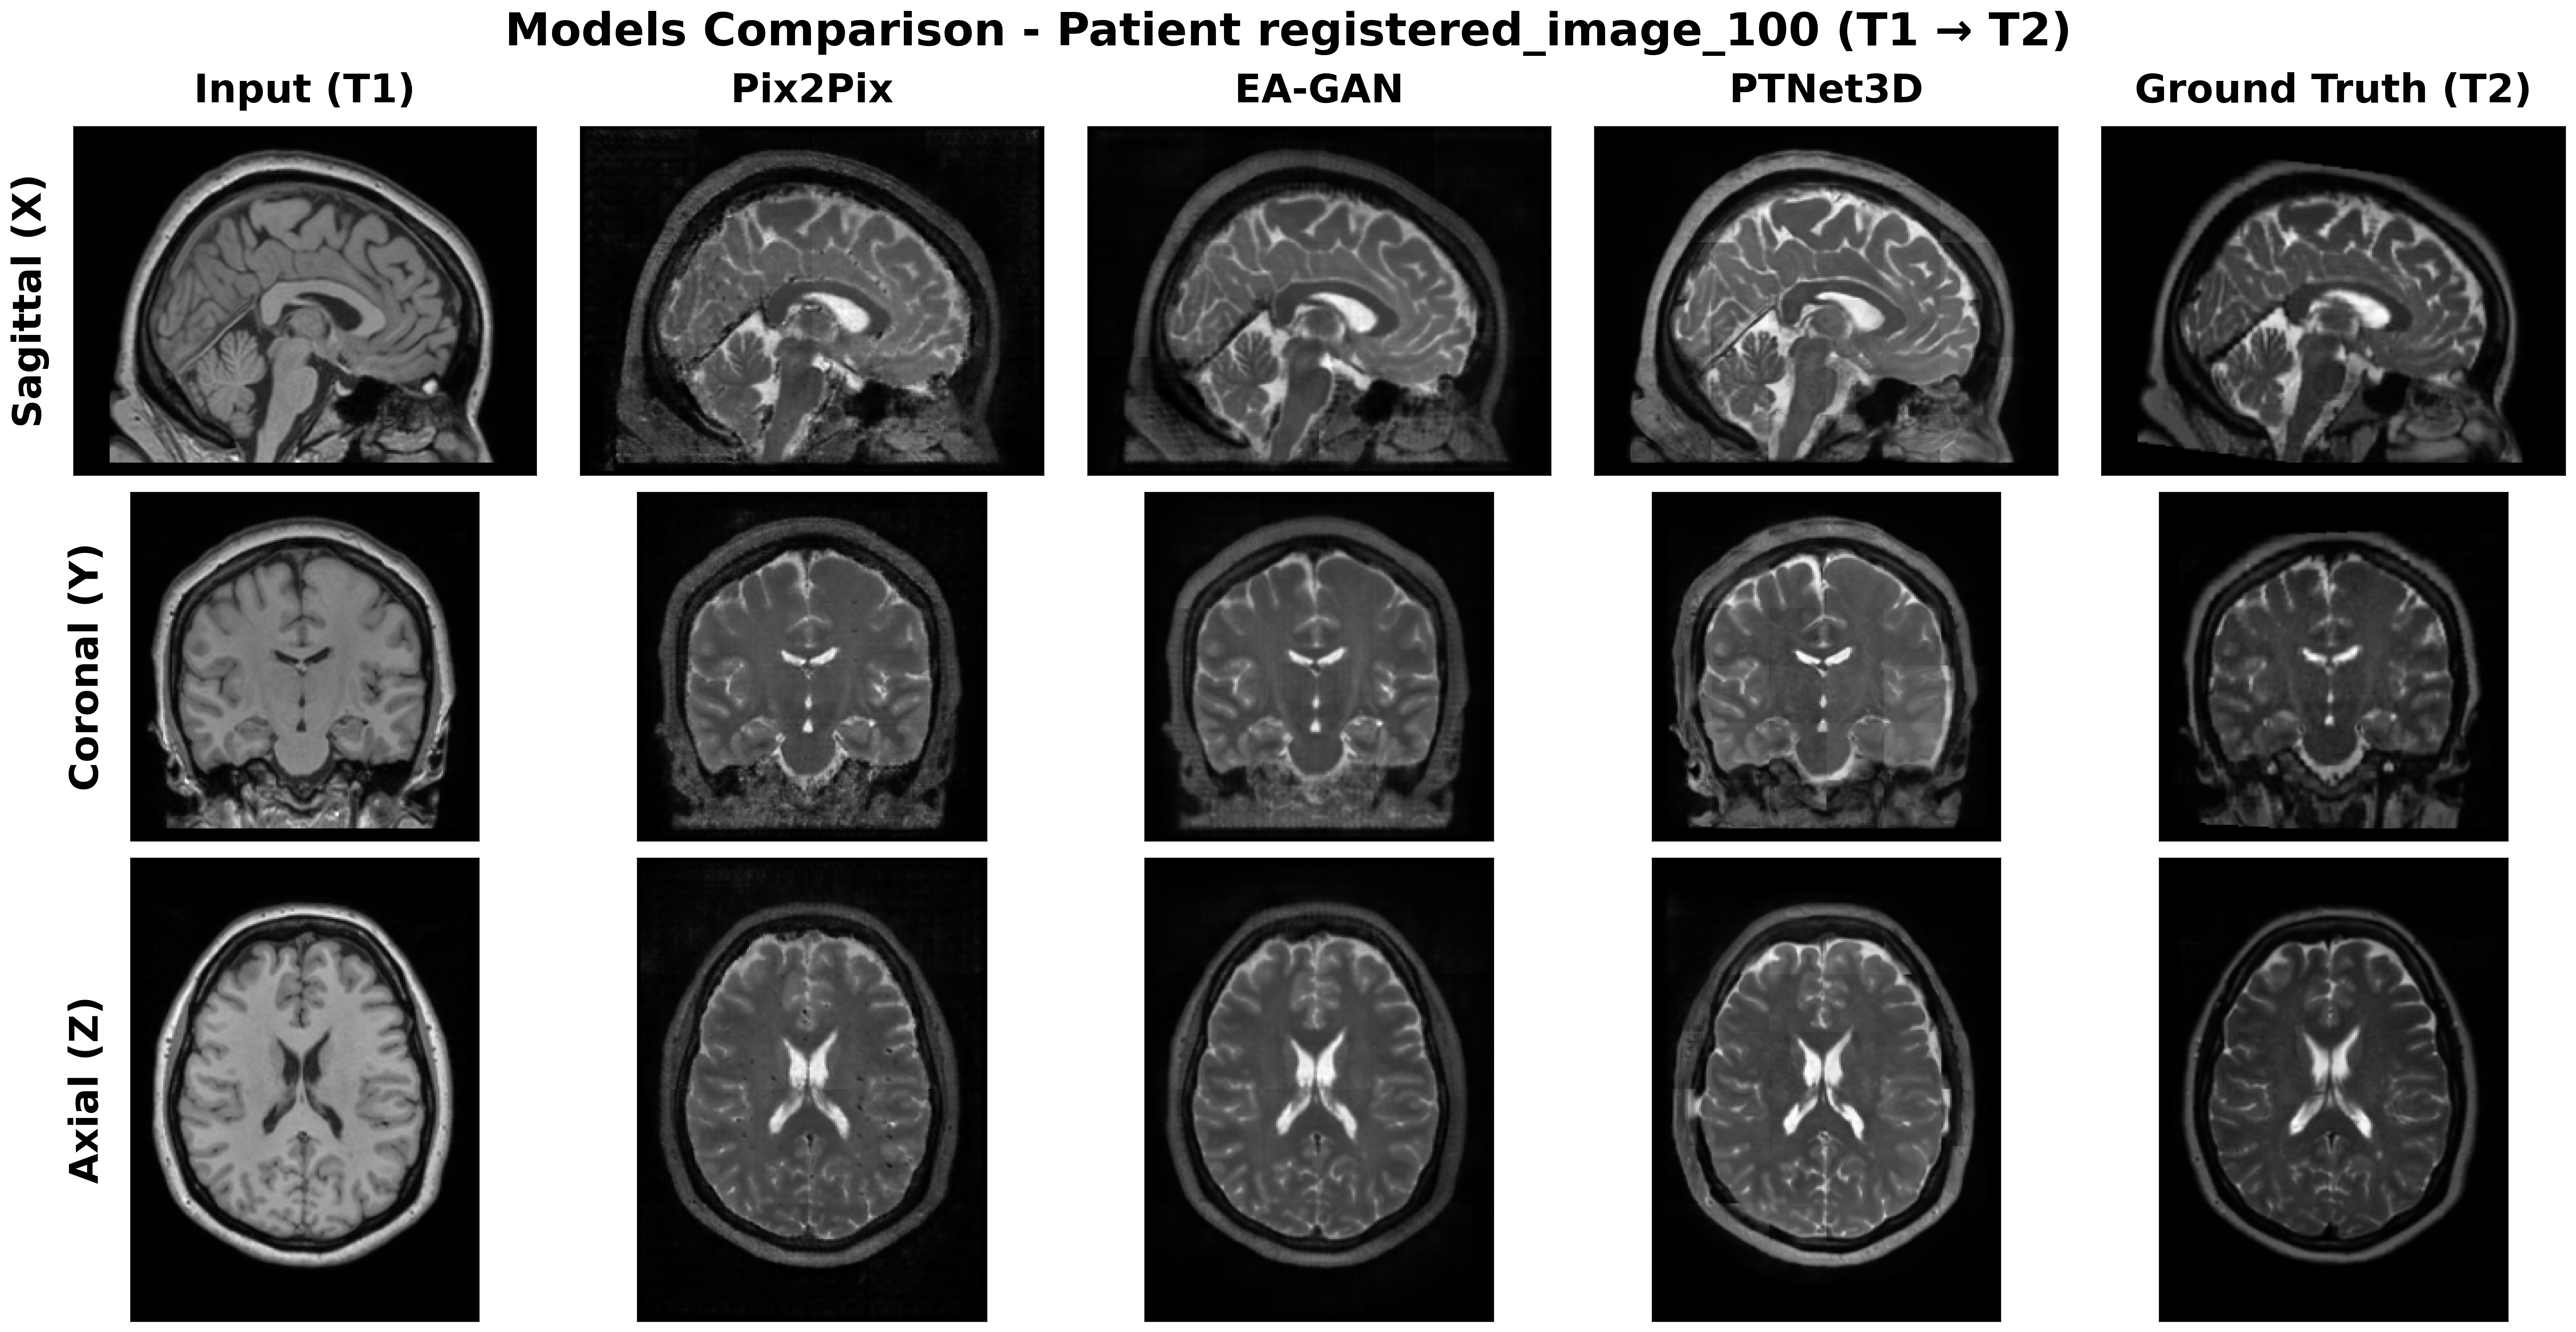
\includegraphics[width=\textwidth]{Images/IXI t1 - t2 .png}
    \caption{Qualitative comparison of \textbf{T1 $\rightarrow$ T2} translation on a subject from the external \textbf{IXI dataset}. From left to right: Source T1, Pix2Pix, Ea-GAN, PTNet3D, and Ground Truth T2.}
    \label{fig:qual_t1_t2}
\end{figure}

\begin{figure}[H]
    \centering
    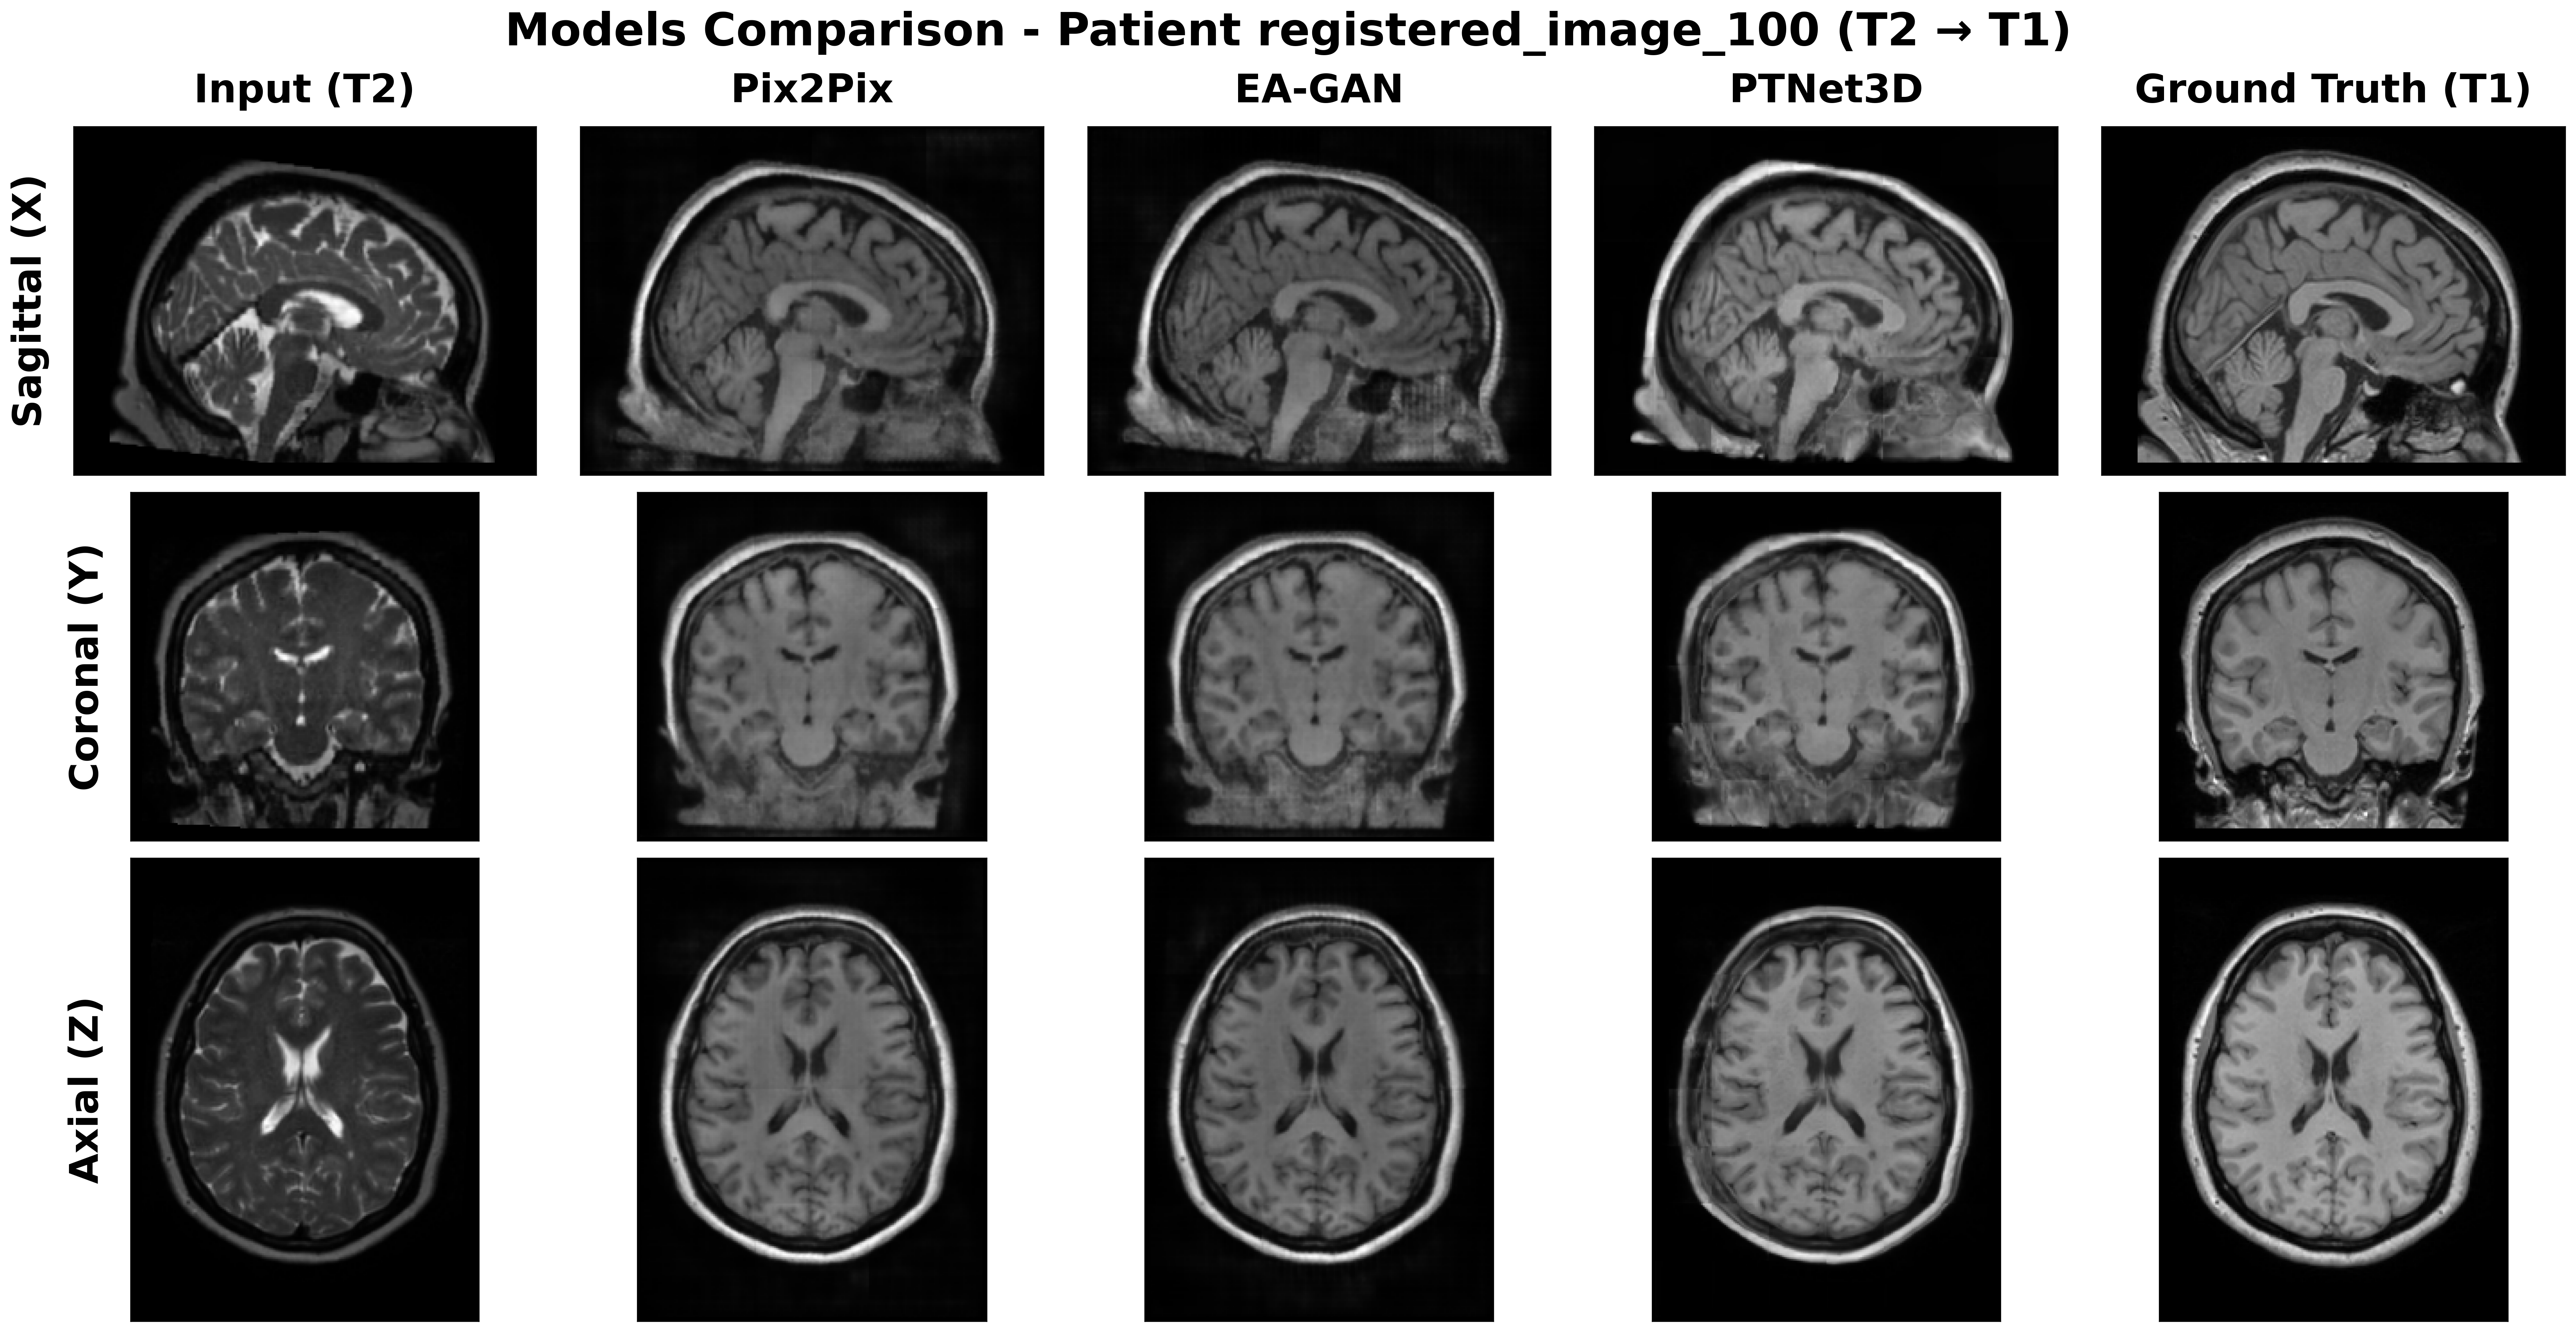
\includegraphics[width=\textwidth]{Images/IXI t2 - t1.png}
    \caption{Qualitative comparison of \textbf{T2 $\rightarrow$ T1} translation on a subject from the external \textbf{IXI dataset}. From left to right: Source T2, Pix2Pix, Ea-GAN, PTNet3D, and Ground Truth T1.}
    \label{fig:qual_t2_t1}
\end{figure}


\subsubsection*{T1 $\leftrightarrow$ FLAIR Translation (OpenNeuro Dataset)}
Figures \ref{fig:qual_t1_flair} and \ref{fig:qual_flair_t1} illustrate the T1$\leftrightarrow$FLAIR translation capabilities on the out-of-distribution OpenNeuro dataset.

\begin{figure}[H]
    \centering
    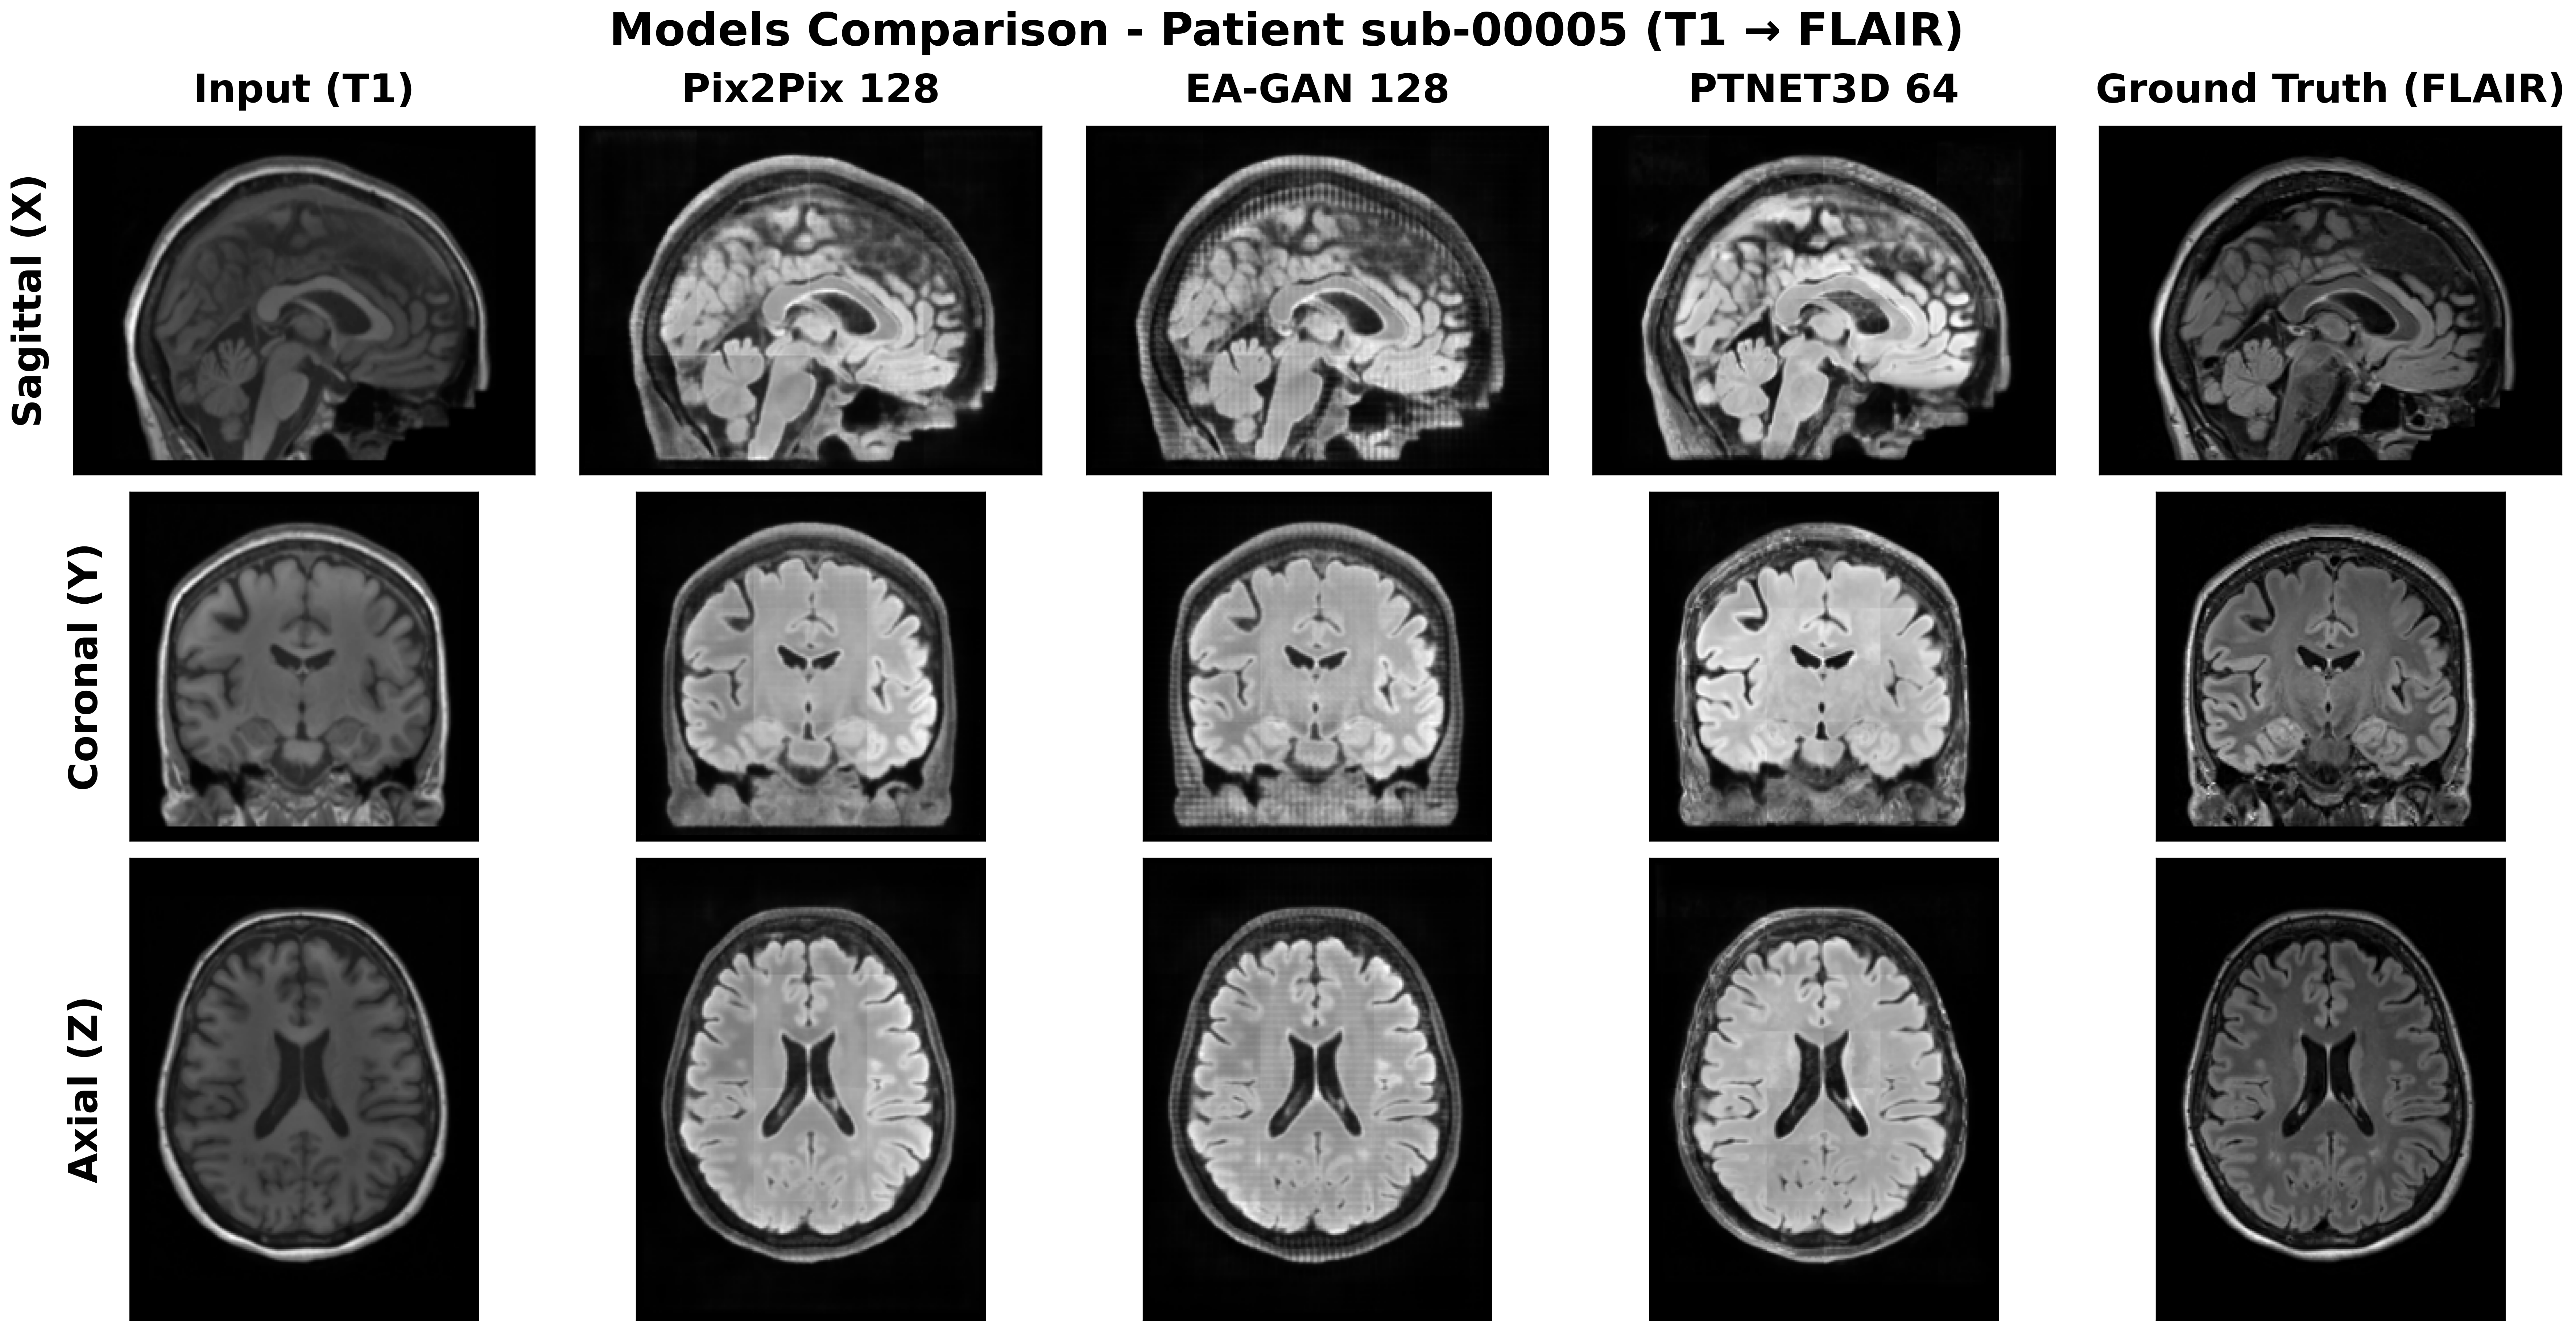
\includegraphics[width=\textwidth]{Images/FCD T1 - Flair.png}
    \caption{Qualitative comparison of \textbf{T1 $\rightarrow$ FLAIR} translation on a subject from the external \textbf{OpenNeuro dataset}. Source T1, Pix2Pix, Ea-GAN, PTNet3D, and Ground Truth FLAIR.}
    \label{fig:qual_t1_flair}
\end{figure}

\begin{figure}[H]
    \centering
    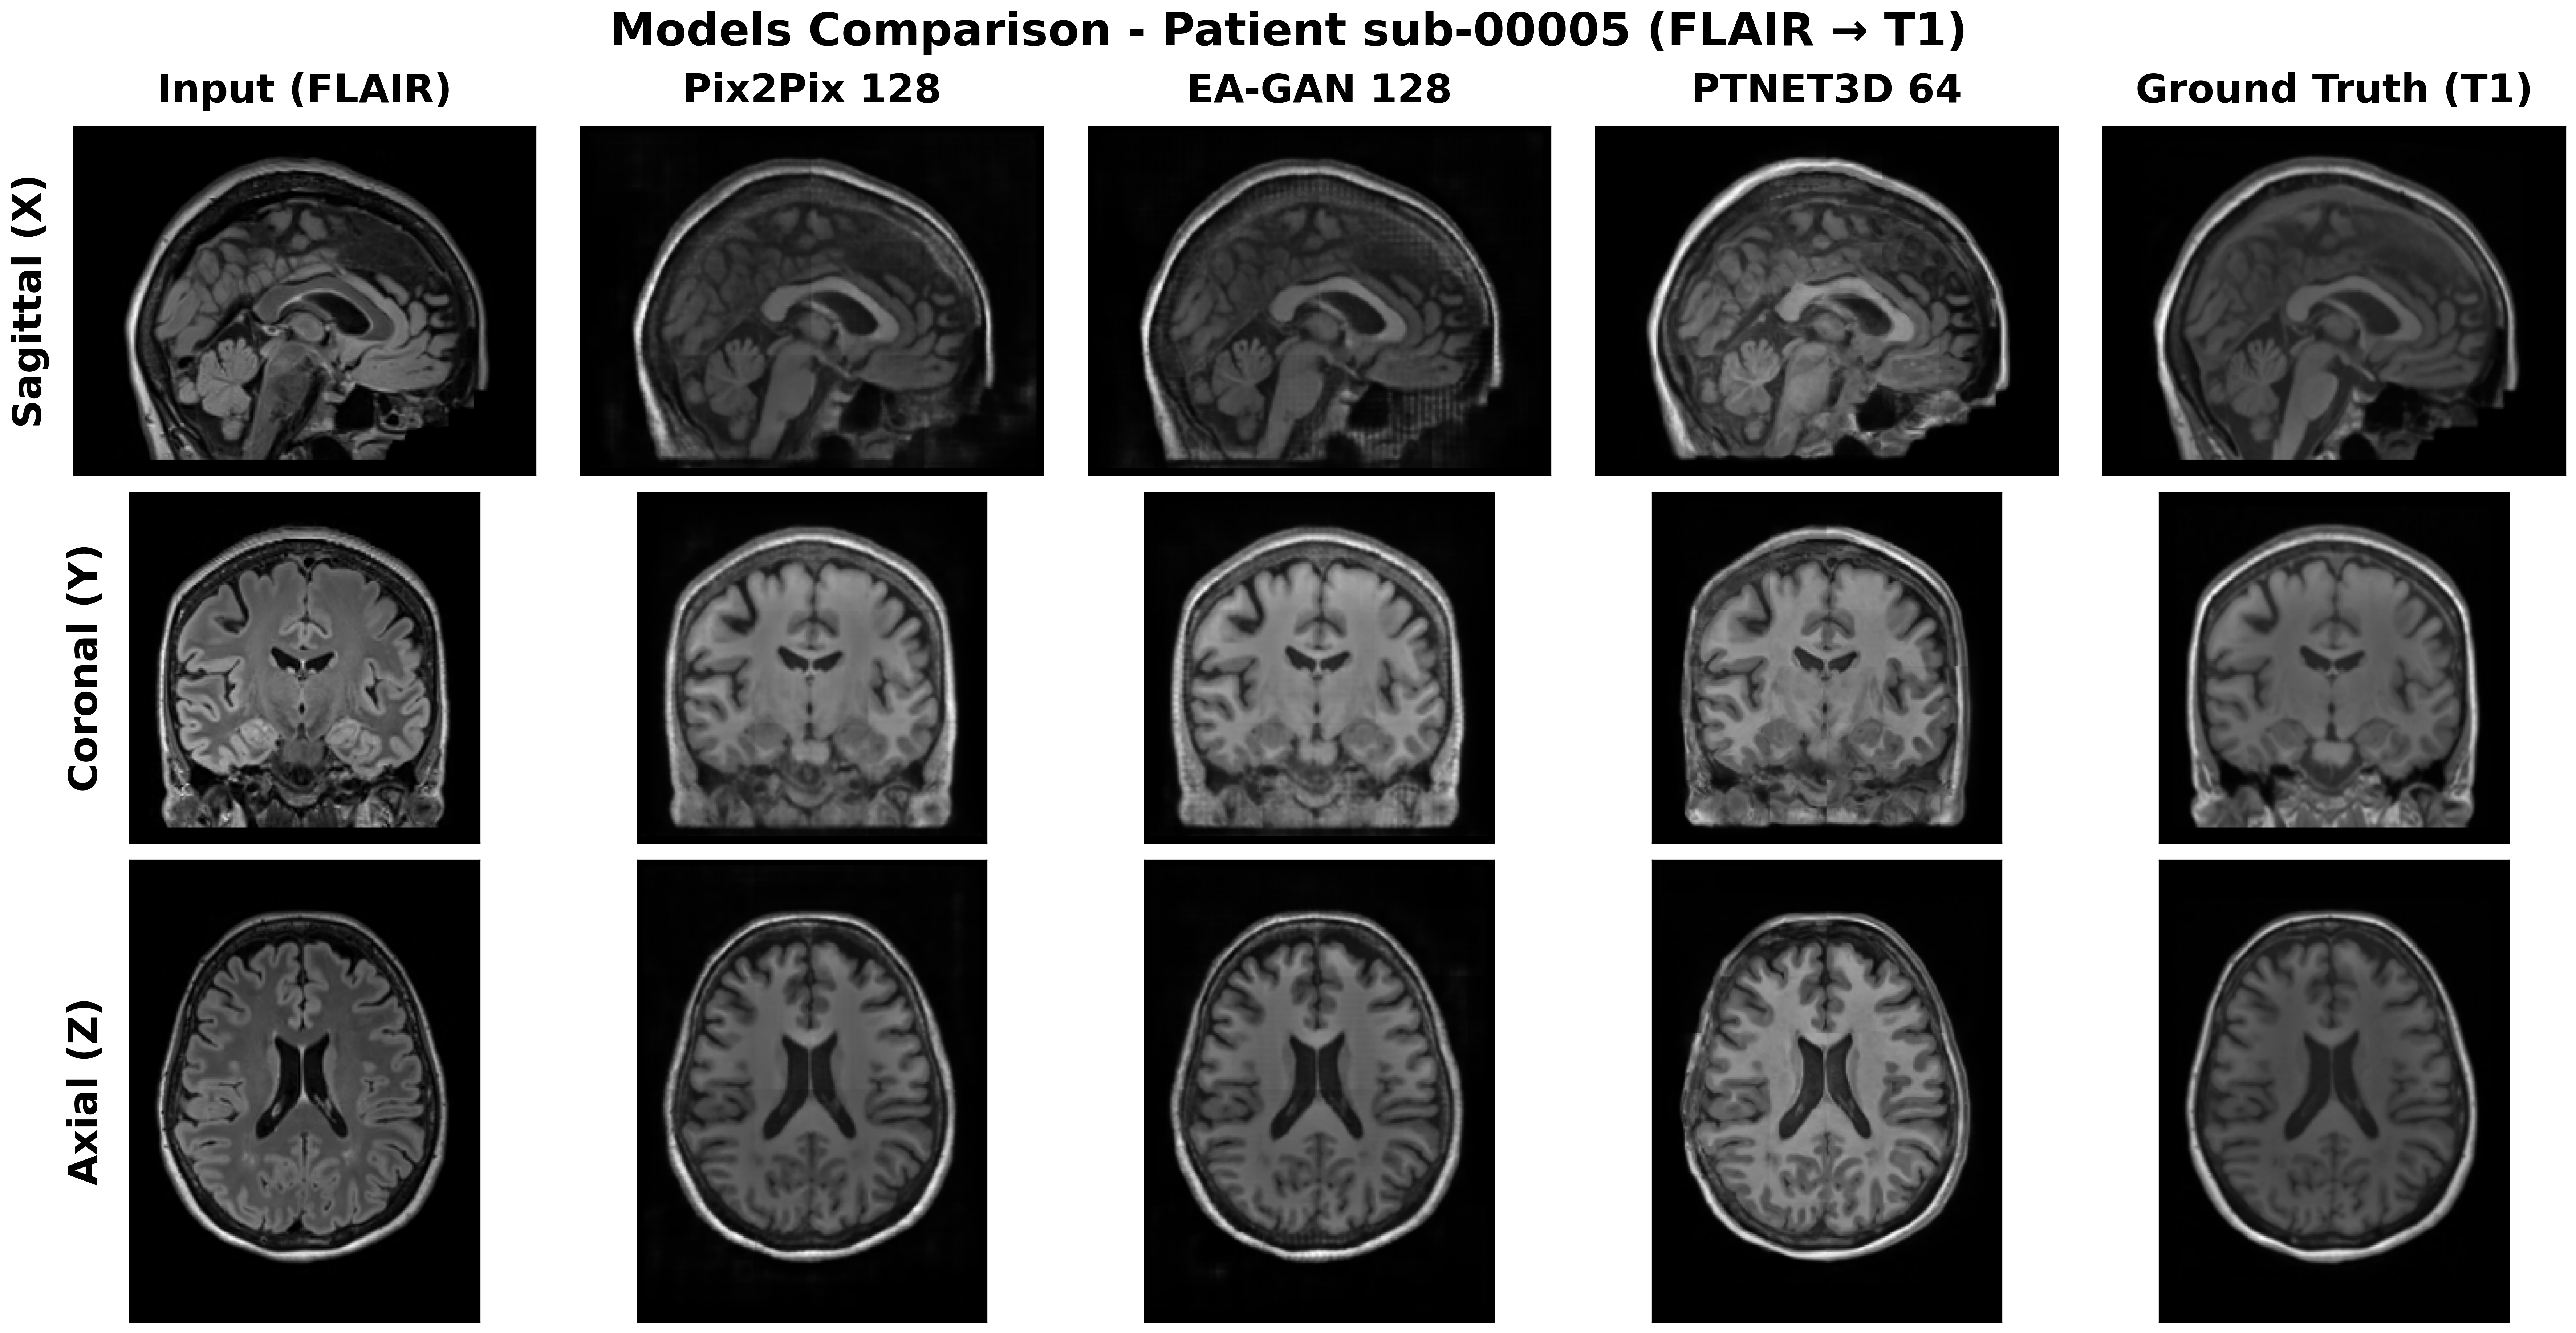
\includegraphics[width=\textwidth]{Images/FCD FLAIR - T1 .png}
    \caption{Qualitative comparison of \textbf{FLAIR $\rightarrow$ T1} translation on a subject from the external \textbf{OpenNeuro dataset}. From left to right: Source FLAIR, Pix2Pix, Ea-GAN, PTNet3D, and Ground Truth T1.}
    \label{fig:qual_flair_t1}
\end{figure}


\subsubsection*{T2 $\leftrightarrow$ FLAIR Translation (ADNI Dataset)}
Since external paired data for the T2$\leftrightarrow$FLAIR modalities was not available, Figures \ref{fig:qual_t2_flair} and \ref{fig:qual_flair_t2} showcase the synthesis quality exclusively on the internal ADNI test cohort.

\begin{figure}[H]
    \centering
    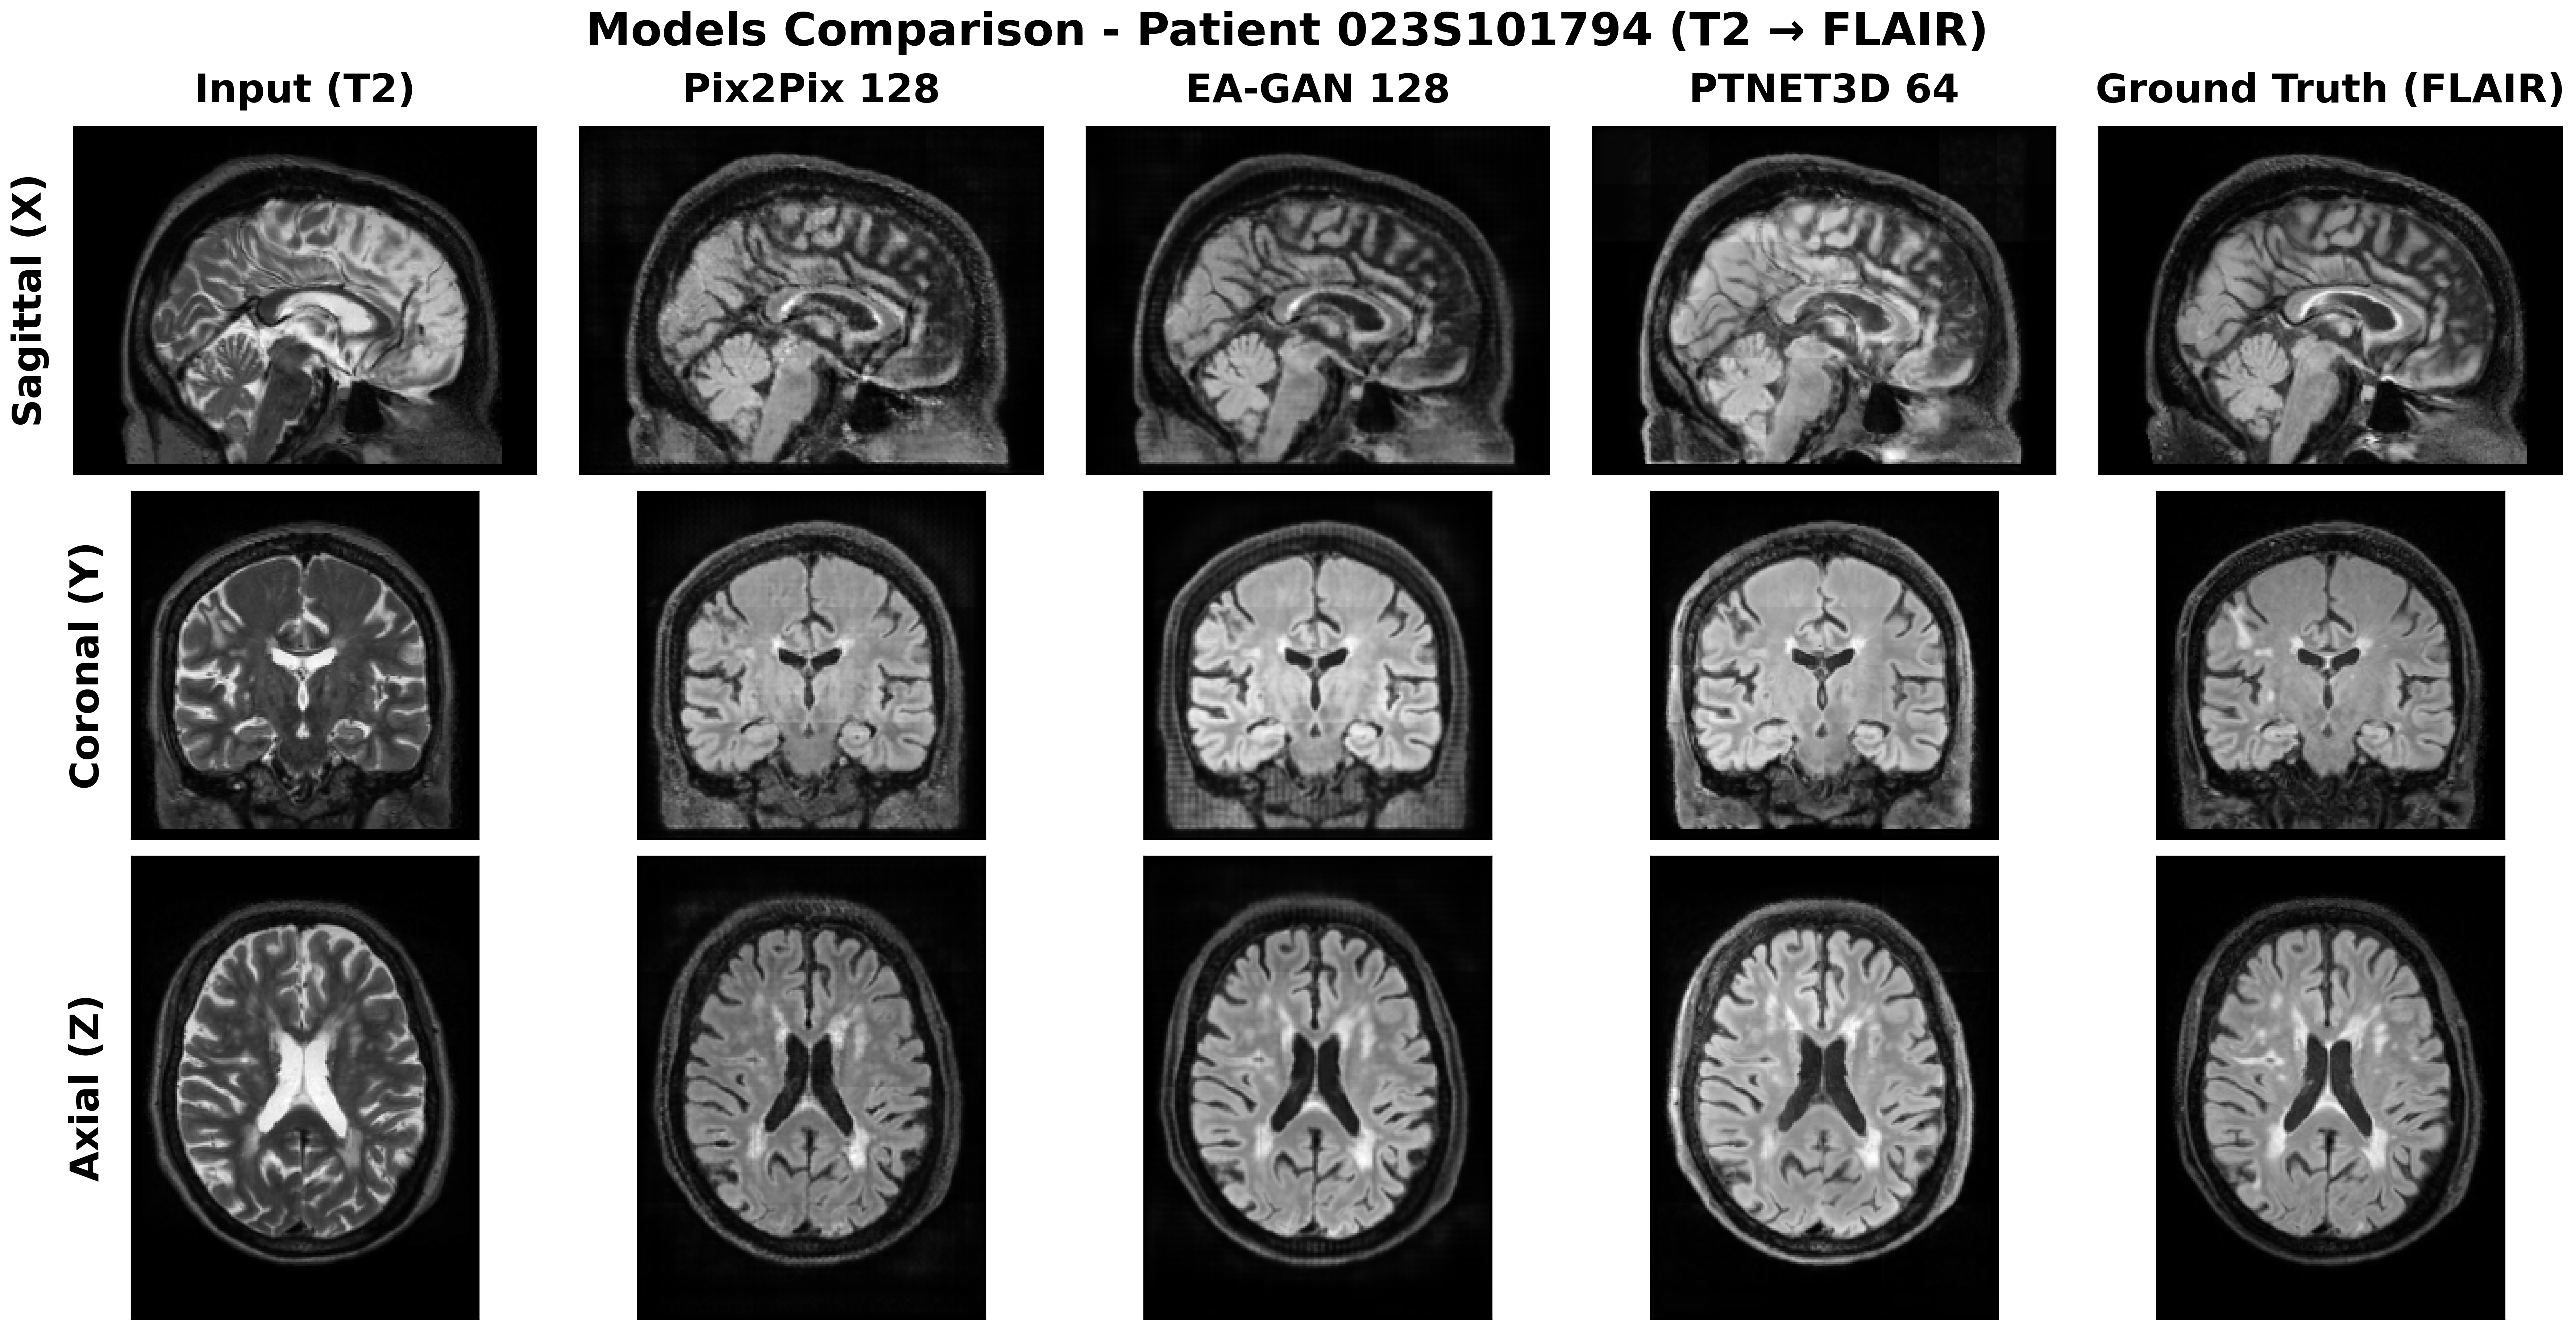
\includegraphics[width=\textwidth]{Images/ADNI t2 - flair .png}
    \caption{Qualitative comparison of \textbf{T2 $\rightarrow$ FLAIR} translation on a subject from the internal \textbf{ADNI dataset}. From left to right: Source T2, Pix2Pix, Ea-GAN, PTNet3D, and Ground Truth FLAIR.}
    \label{fig:qual_t2_flair}
\end{figure}

\begin{figure}[H]
    \centering
    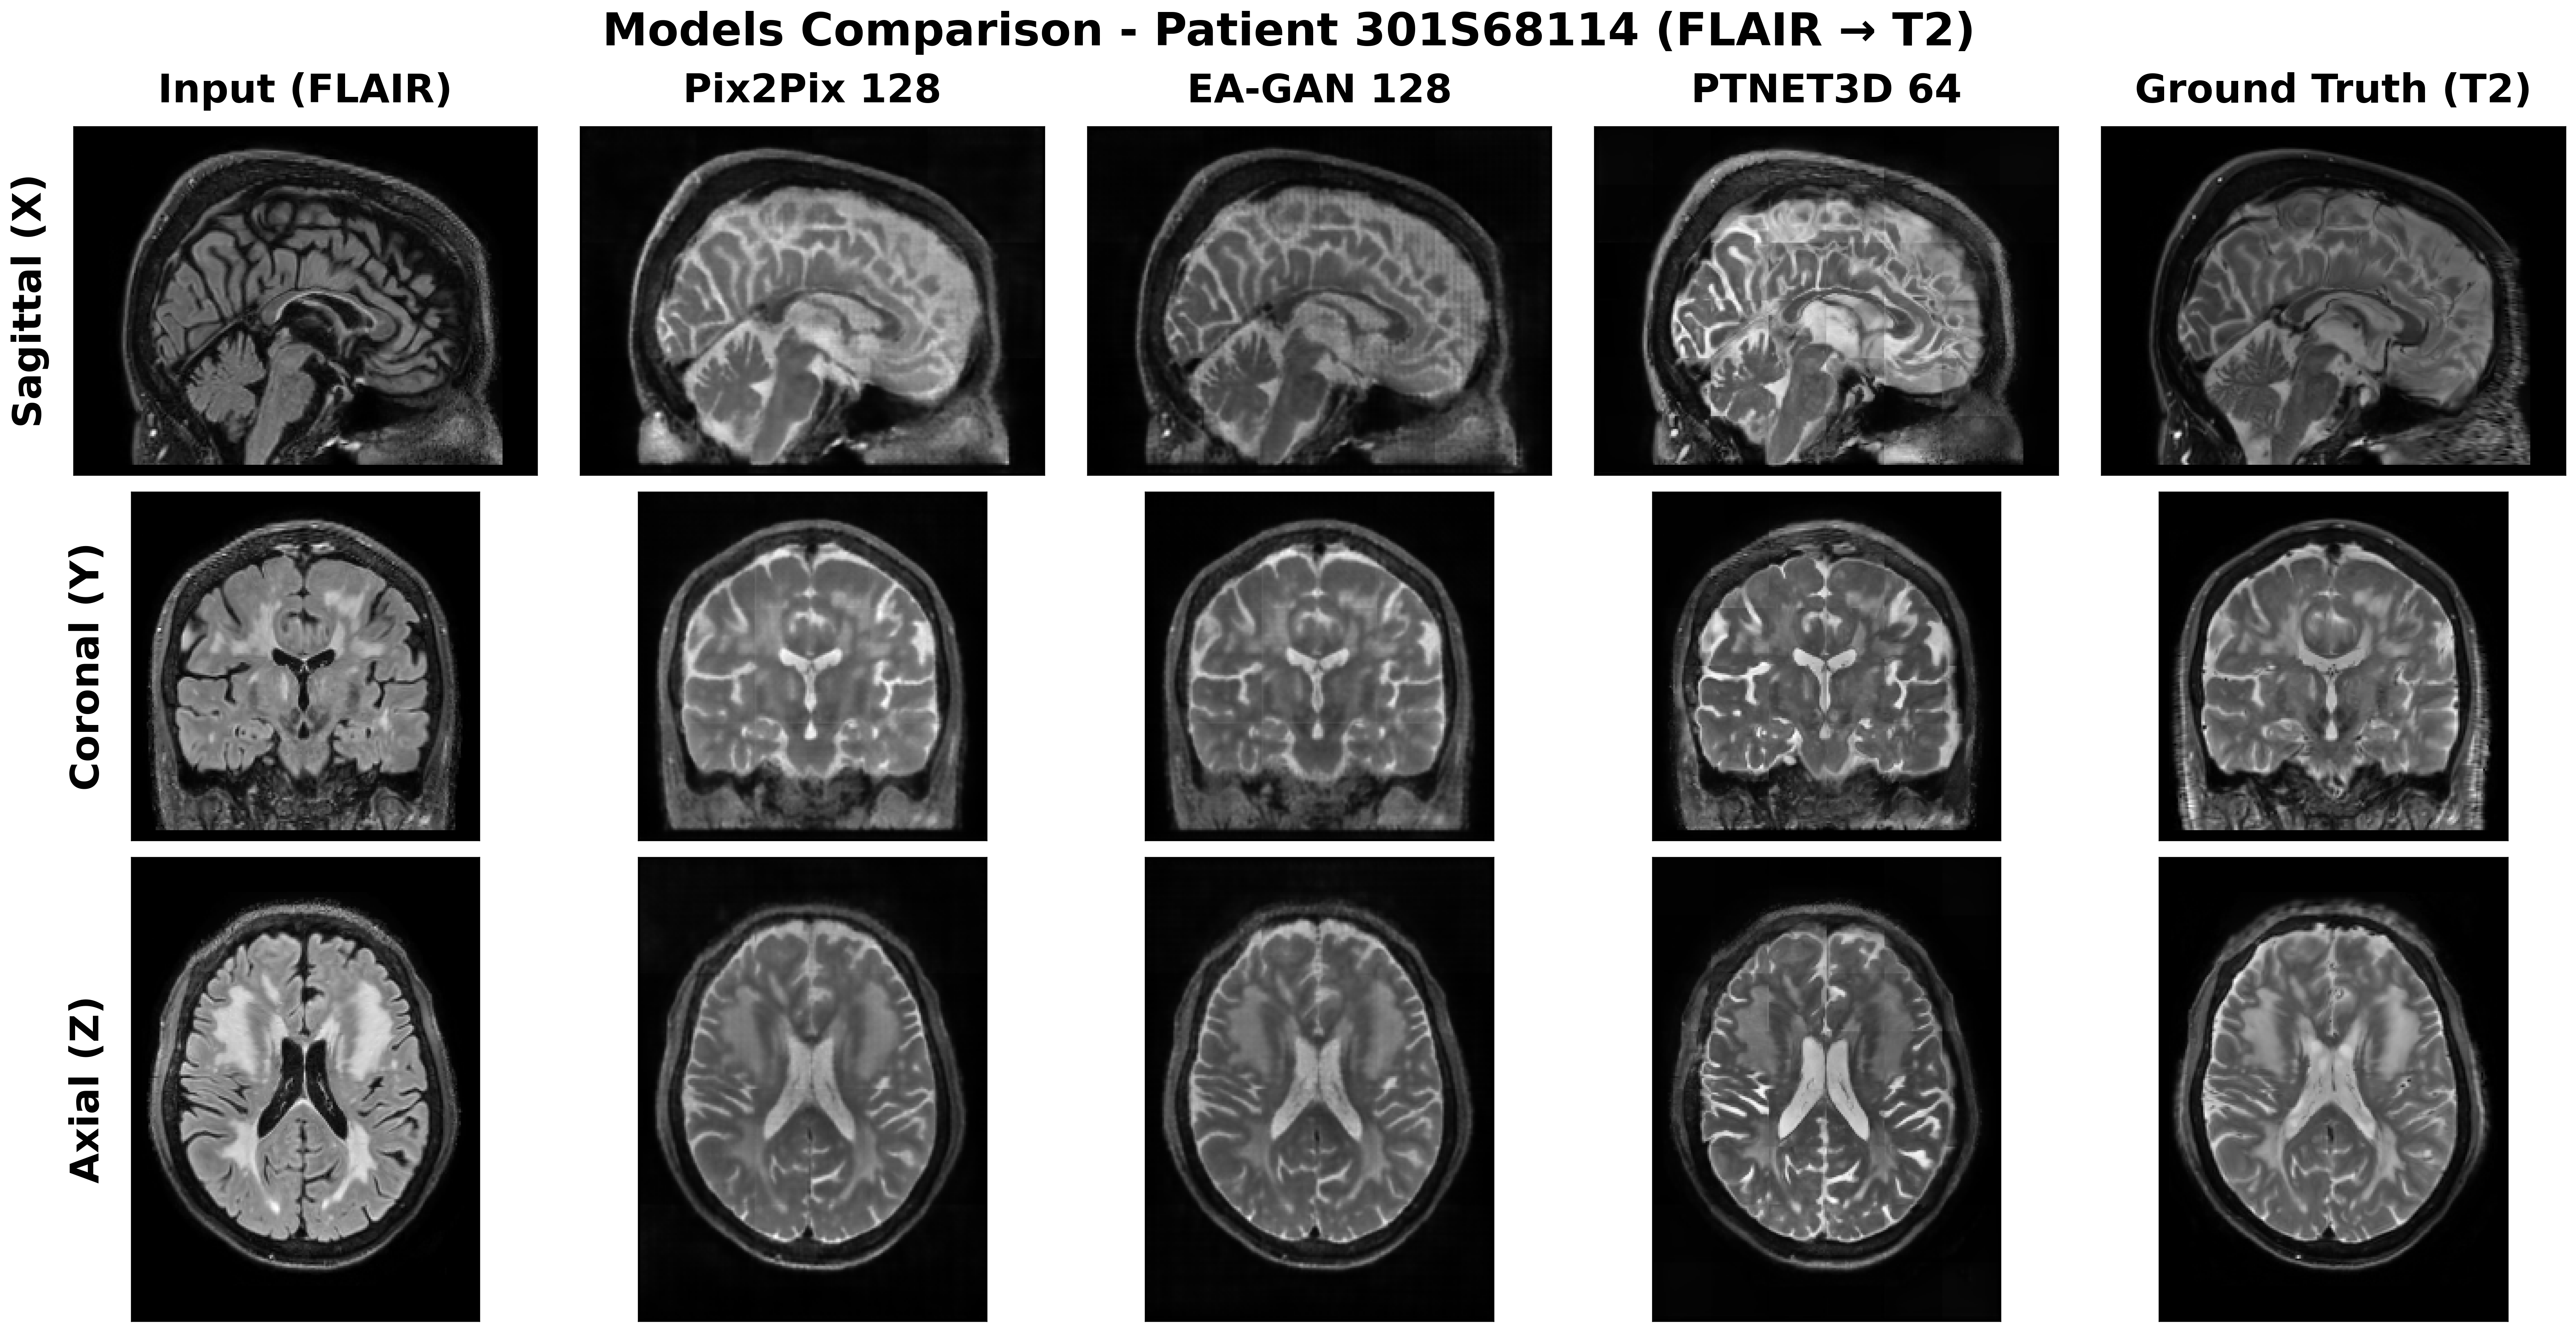
\includegraphics[width=\textwidth]{Images/adnii flair - t2.png}
    \caption{Qualitative comparison of \textbf{FLAIR $\rightarrow$ T2} translation on a subject from the internal \textbf{ADNI dataset}. From left to right: Source FLAIR, Pix2Pix, Ea-GAN, PTNet3D, and Ground Truth T2.}
    \label{fig:qual_flair_t2}
\end{figure}


\subsection{Downstream Task Results}

To evaluate the clinical validity and anatomical fidelity of the synthesized volumes, we tested their performance on two distinct downstream tasks: Brain Age Estimation (on the IXI dataset) and Epilepsy Classification (HC vs FCD on the OpenNeuro dataset).

\paragraph{Task 1: Brain Age Estimation (IXI)}
The results of the Leave-One-Site-Out Cross-Validation (LOSO-CV) for brain age estimation are presented for both translation directions. Table~\ref{tab:age_ixi_t1} reports the Mean Absolute Error (MAE) when training the SFCN model on real T1 scans versus synthetic T1 scans (generated from T2) and a hybrid data augmentation setup. Similarly, Table~\ref{tab:age_ixi_t2} presents the downstream performance for the T2 modalities (synthesized from T1). 

\begin{table}[H]
\centering
\resizebox{\textwidth}{!}{%
\begin{tabular}{lccccc}
\hline\hline\noalign{\smallskip}
\textbf{Training Setup} & \textbf{Guys MAE ($\downarrow$)} & \textbf{HH MAE ($\downarrow$)} & \textbf{IOP MAE ($\downarrow$)} & \textbf{Total MAE ($\downarrow$)} & \textbf{Pearson $r$ ($\uparrow$)} \\
\noalign{\smallskip}\hline\noalign{\smallskip}
Real T1 (Baseline) & $6.17$ & $6.86$ & $7.36$ & $6.54$ & $0.881$ \\
\hline\noalign{\smallskip}
Synthetic T1 (Pix2Pix) & $6.41$ & $7.74$ & $8.21$ & $7.06$ & $0.861$ \\
Synthetic T1 (Ea-GAN)  & $6.36$ & $6.53$ & $7.75$ & $6.59$ & $0.873$ \\
Synthetic T1 (PTNet3D) & $6.30$ & $6.43$ & $8.69$ & $6.64$ & $0.881$ \\
\hline\noalign{\smallskip}
Hybrid T1 (Pix2Pix + Real) & $5.75$ & $5.34$ & $6.24$ & $5.68$ & $\mathbf{0.912}$ \\
Hybrid T1 (Ea-GAN + Real)  & $\mathbf{4.84}$ & $\mathbf{5.00}$ & $8.03$ & $\mathbf{5.28}$ & $0.908$ \\
Hybrid T1 (PTNet3D + Real) & $5.39$ & $6.07$ & $\mathbf{6.16}$ & $5.70$ & $0.905$ \\
\hline\hline
\end{tabular}%
}
\vspace{2mm}
\caption{Downstream performance (Brain Age Estimation) for the \textbf{T2 $\rightarrow$ T1} translation. The table compares the MAE and Pearson correlation coefficient of the SFCN model evaluated through LOSO-CV (Guys, HH, IOP) when trained on Real T1 scans, purely Synthetic T1 scans, and a Hybrid data augmentation setup. The best results for each column are highlighted in \textbf{bold}.}
\label{tab:age_ixi_t1}
\end{table}

\begin{table}[H]
\centering
\resizebox{\textwidth}{!}{%
\begin{tabular}{lccccc}
\hline\hline\noalign{\smallskip}
\textbf{Training Setup} & \textbf{Guys MAE ($\downarrow$)} & \textbf{HH MAE ($\downarrow$)} & \textbf{IOP MAE ($\downarrow$)} & \textbf{Total MAE ($\downarrow$)} & \textbf{Pearson $r$ ($\uparrow$)} \\
\noalign{\smallskip}\hline\noalign{\smallskip}
Real T2 (Baseline) & $6.45$ & $5.87$ & $6.70$ & $6.29$ & $0.889$ \\
\hline\noalign{\smallskip}
Synthetic T2 (Pix2Pix) & $10.42$ & $10.18$ & $8.43$ & $10.10$ & $0.730$ \\
Synthetic T2 (Ea-GAN)  & $10.22$ & $10.22$ & $7.55$ & $9.89$ & $0.773$ \\
Synthetic T2 (PTNet3D) & $9.54$ & $9.11$ & $9.86$ & $9.44$ & $0.781$ \\
\hline\noalign{\smallskip}
Hybrid T2 (Pix2Pix + Real) & $5.52$ & $4.77$ & $4.38$ & $5.14$ & $0.922$ \\
Hybrid T2 (Ea-GAN + Real)  & $5.43$ & $4.79$ & $4.36$ & $5.09$ & $0.921$ \\
Hybrid T2 (PTNet3D + Real) & $\mathbf{4.91}$ & $\mathbf{4.76}$ & $\mathbf{4.33}$ & $\mathbf{4.79}$ & $\mathbf{0.932}$ \\
\hline\hline
\end{tabular}%
}
\vspace{2mm}
\caption{Downstream performance (Brain Age Estimation) for the \textbf{T1 $\rightarrow$ T2} translation. The table compares the MAE and Pearson correlation coefficient of the SFCN model evaluated through LOSO-CV (Guys, HH, IOP) when trained on Real T2 scans, purely Synthetic T2 scans, and a Hybrid data augmentation setup. The best results for each column are highlighted in \textbf{bold}.}
\label{tab:age_ixi_t2}
\end{table}

\paragraph{Task 2: Epilepsy Classification (OpenNeuro)}
For the binary classification task (Healthy Controls vs Focal Cortical Dysplasia), the aggregate metrics of the 5-Fold Cross-Validation are detailed in Tables~\ref{tab:epilepsy_openneuro_t1} and \ref{tab:epilepsy_openneuro_flair}. These tables highlight the global Accuracy and ROC-AUC scores across the different experimental setups: the Real baseline, models trained on synthetic data and evaluated on both Real and Synthetic validation scans, and the Hybrid data augmentation configuration. This comprehensive comparison allows us to verify both the internal consistency of the synthesized representations and their clinical viability when tested against real clinical scans.

\begin{table}[H]
\centering
\resizebox{\textwidth}{!}{%
\begin{tabular}{l c ccc ccc ccc}
\hline\hline\noalign{\smallskip}
\multirow{2}{*}{\textbf{Metric}} & \textbf{Baseline} & \multicolumn{3}{c}{\textbf{Synthetic (Test: Real)}} & \multicolumn{3}{c}{\textbf{Synthetic (Test: Syn)}} & \multicolumn{3}{c}{\textbf{Hybrid (Test: Real)}} \\
\cline{2-2} \cline{3-5} \cline{6-8} \cline{9-11}\noalign{\smallskip}
& Real & Pix2Pix & Ea-GAN & PTNet3D & Pix2Pix & Ea-GAN & PTNet3D & Pix2Pix & Ea-GAN & PTNet3D \\
\noalign{\smallskip}\hline\noalign{\smallskip}
Accuracy ($\uparrow$) & $0.700$ & $0.647$ & $0.506$ & $0.535$ & $0.747$ & $0.753$ & $0.735$ & $\mathbf{0.765}$ & $0.735$ & $0.700$ \\
ROC-AUC ($\uparrow$)  & $0.815$ & $0.707$ & $0.519$ & $0.558$ & $0.758$ & $0.809$ & $0.823$ & $\mathbf{0.841}$ & $0.798$ & $0.802$ \\
\hline\hline
\end{tabular}%
}
\vspace{2mm}
\caption{Downstream performance (Epilepsy Classification) for the \textbf{FLAIR $\rightarrow$ T1} translation across 5-Fold Cross-Validation. Results compare the Real baseline, models trained on synthetic data (tested on both Real and Synthetic scans), and the Hybrid data augmentation setup. The best result for each metric is highlighted in \textbf{bold}.}
\label{tab:epilepsy_openneuro_t1}
\end{table}

\begin{table}[H]
\centering
\resizebox{\textwidth}{!}{%
\begin{tabular}{l c ccc ccc ccc}
\hline\hline\noalign{\smallskip}
\multirow{2}{*}{\textbf{Metric}} & \textbf{Baseline} & \multicolumn{3}{c}{\textbf{Synthetic (Test: Real)}} & \multicolumn{3}{c}{\textbf{Synthetic (Test: Syn)}} & \multicolumn{3}{c}{\textbf{Hybrid (Test: Real)}} \\
\cline{2-2} \cline{3-5} \cline{6-8} \cline{9-11}\noalign{\smallskip}
& Real & Pix2Pix & Ea-GAN & PTNet3D & Pix2Pix & Ea-GAN & PTNet3D & Pix2Pix & Ea-GAN & PTNet3D \\
\noalign{\smallskip}\hline\noalign{\smallskip}
Accuracy ($\uparrow$) & $0.765$ & $0.453$ & $0.523$ & $0.494$ & $0.747$ & $0.729$ & $0.735$ & $0.776$ & $0.765$ & $\mathbf{0.782}$ \\
ROC-AUC ($\uparrow$)  & $0.800$ & $0.347$ & $0.505$ & $0.461$ & $0.823$ & $0.798$ & $0.835$ & $0.835$ & $0.819$ & $\mathbf{0.849}$ \\
\hline\hline
\end{tabular}%
}
\vspace{2mm}
\caption{Downstream performance (Epilepsy Classification) for the \textbf{T1 $\rightarrow$ FLAIR} translation across 5-Fold Cross-Validation. Results compare the Real baseline, models trained on synthetic data (tested on both Real and Synthetic scans), and the Hybrid data augmentation setup. The best result for each metric is highlighted in \textbf{bold}.}
\label{tab:epilepsy_openneuro_flair}
\end{table}


\subsection{Discussion}

\paragraph{Performance on the Internal Cohort (ADNI)}
When evaluated on the ADNI internal test set, where the underlying data distribution closely matches the training set, the Convolutional Neural Networks (Pix2Pix and Ea-GAN) consistently outperform the transformer-based architecture (PTNet3D) across all translation tasks and directions. 

Between the two CNNs, the standard Pix2Pix baseline demonstrates strong performance in purely voxel-wise intensity metrics, frequently achieving the highest PSNR and lowest MAE (e.g., in T1$\rightarrow$T2 and T2$\rightarrow$FLAIR). However, Ea-GAN distinctly excels in structural and perceptual fidelity. Thanks to the integration of the edge-aware loss mechanism, Ea-GAN consistently secures the best LPIPS, FSIM, and NCC scores. For instance, in the FLAIR$\rightarrow$T2 task, Ea-GAN achieves a clean sweep, outperforming the competitors on every single metric, including a remarkable SSIM of $0.827$ and LPIPS of $0.068$. 

Conversely, PTNet3D struggles to compete in the intra-domain setting. It exhibits significantly higher MAE and lower PSNR across all tasks, indicating that the volumetric transformer likely requires either vastly larger training datasets or longer training schedules to match the high-frequency texture synthesis capabilities of CNNs on a specific, narrow domain.

\paragraph{Cross-Domain Generalization (IXI and OpenNeuro)}
Testing the models on the external IXI and OpenNeuro datasets reveals a general and expected degradation in absolute performance across the architectures. This is primarily due to the domain shift introduced by different MRI scanners, magnetic field strengths, and sequence acquisition protocols. For example, when evaluating the T1$\rightarrow$T2 translation on the IXI dataset, the SSIM drops sharply from $\sim 0.84$ (on the internal ADNI cohort) to $\sim 0.69$, while the MAE effectively doubles from $\sim 0.05$ to $\sim 0.10$.


However, this cross-domain evaluation exposes a critical and counter-intuitive behavior regarding PTNet3D. While the CNNs suffer performance drops on the external datasets, the transformer-based PTNet3D demonstrates remarkable robustness and generalization. On the IXI dataset (T1$\leftrightarrow$T2), PTNet3D surprisingly surpasses both Pix2Pix and Ea-GAN in Structural Similarity (SSIM) in both translation directions (achieving $0.715$ and $0.766$), despite remaining inferior in terms of pure absolute error (MAE). Furthermore, on the OpenNeuro dataset, PTNet3D achieves the best NCC ($0.848$) in the T1$\rightarrow$FLAIR translation, proving its capability to maintain a strong linear structural correlation even under a substantial domain shift. 

These results provide a significant architectural insight: while local convolutions (CNNs) are highly efficient at learning and replicating the specific local textures and noise patterns of the training domain, they are inherently prone to overfitting to those specific scanner characteristics. In contrast, the global self-attention mechanism of PTNet3D appears to capture broader, domain-agnostic anatomical structures, allowing the model to better preserve the macroscopic structural integrity of the brain when exposed to entirely unseen MRI protocols.

\paragraph{Translation Asymmetry and FLAIR Synthesis Difficulty}
An important observation emerging from our quantitative results is the pronounced asymmetry between translation directions involving the FLAIR modality. Across both ADNI and OpenNeuro datasets, synthesizing T1-weighted images from FLAIR consistently yields much higher PSNR and SSIM than the reverse direction (T1$\rightarrow$FLAIR). For instance, on ADNI, FLAIR$\rightarrow$T1 achieves PSNR values of $\sim$24 dB across both CNNs, whereas T1$\rightarrow$FLAIR yields only $\sim$17--18 dB. This asymmetry can be attributed to the fundamental differences in tissue contrast complexity: T1w images exhibit relatively smooth, predictable intensity profiles dominated by grey--white matter contrast, whereas FLAIR images must additionally encode the suppression of cerebrospinal fluid (CSF) and the hyperintense appearance of white matter lesions---features that are inherently more difficult to accurately reconstruct from a T1w source.

Furthermore, the overall degradation in performance on the OpenNeuro dataset likely reflects not only the scanner hardware differences but also the heterogeneous patient population in the FCD cohort, which includes both healthy controls and subjects with focal cortical dysplasia---a condition that introduces localized structural abnormalities.

\paragraph{Computational Efficiency and Practical Considerations}
From a practical deployment perspective, the CNN-based models (Pix2Pix and Ea-GAN) offer a clear advantage. With virtually identical architectures comprising $\sim$178 million trainable parameters, they complete their full $150$-epoch training schedules in $25$--$75$ hours depending on dataset size. In contrast, PTNet3D requires $\sim$84 hours per translation task regardless of dataset size, while operating on smaller $64^3$ patches (versus $128^3$ for the CNNs) due to memory constraints. Paradoxically, despite having far fewer trainable parameters ($\sim$15.5 million), the transformer-based model is more resource-intensive because of the auxiliary frozen networks (33 million frozen parameters from the external 3D ResNet feature extractor) and the quadratic complexity of the bottleneck attention layers.

\paragraph{Downstream Clinical Utility}
The downstream evaluation on brain age estimation (\autoref{tab:age_ixi_t1} and \autoref{tab:age_ixi_t2}) demonstrates the clinical viability and anatomical fidelity of the synthesized volumes.
In the purely synthetic training regime, a pronounced directional asymmetry is observed. For \textbf{T2 $\rightarrow$ T1} translation (\autoref{tab:age_ixi_t1}), synthetic scans nearly replicate the native real baseline ($\text{MAE} = 6.54$ years, $r = 0.881$), with Ea-GAN ($6.59$ years) and PTNet3D ($6.64$ years, $r = 0.881$) preserving critical atrophy patterns. Conversely, \textbf{T1 $\rightarrow$ T2} synthesis (\autoref{tab:age_ixi_t2}) entails a larger domain penalty ($\text{MAE} \approx 9.44$--$10.10$ years), though PTNet3D preserves global structure best ($9.44$ years, $r = 0.781$) via self-attention.

Crucially, the \textbf{hybrid augmentation} regime (Real + Synthetic) systematically surpasses the real baselines in both directions. In T2 $\rightarrow$ T1, hybrid models reduce the total MAE to $\mathbf{5.28}$ years (Ea-GAN + Real) and elevate correlation to $r = \mathbf{0.912}$ (Pix2Pix + Real). In T1 $\rightarrow$ T2, PTNet3D + Real achieves a clean sweep across all acquisition sites, reducing the MAE to $\mathbf{4.79}$ years ($\sim 24\%$ error reduction) with $r = \mathbf{0.932}$. These results confirm that intra-sequence synthesis effectively regularizes downstream networks against scanner-induced domain shifts, yielding substantial gains in clinical predictive accuracy.

A remarkably consistent pattern emerges from the binary classification of Focal Cortical Dysplasia on the OpenNeuro dataset (\autoref{tab:epilepsy_openneuro_t1} and \autoref{tab:epilepsy_openneuro_flair}), extending these conclusions from macroscopic morphological regression to subtle pathology detection. When evaluating classifiers within a fully synthetic regime (Test: Synthetic), the models exhibit high internal consistency, achieving up to $0.753$ Accuracy and $0.823$ ROC-AUC in FLAIR $\rightarrow$ T1, and $0.747$ Accuracy with $0.835$ ROC-AUC in T1 $\rightarrow$ FLAIR. This demonstrates that the generative architectures successfully capture and encode the localized structural hallmarks of FCD (such as cortical thickening and blurred grey--white matter junctions) rather than smoothing them away. However, testing these purely synthetic-trained classifiers directly on real patient scans reveals an evident domain gap---most prominently in T1 $\rightarrow$ FLAIR (Accuracy $\sim 0.45$--$0.52$), where subtle intensity discrepancies in synthetic FLAIR contrast hinder direct zero-shot transfer.

Most importantly, the \textbf{hybrid augmentation} strategy once again proves exceptionally effective, systematically establishing new performance ceilings across both translation directions. For FLAIR $\rightarrow$ T1 (\autoref{tab:epilepsy_openneuro_t1}), augmenting real scans with synthetic Pix2Pix data improves classification Accuracy from $0.700$ to $\mathbf{0.765}$ ($+6.5\%$) and ROC-AUC from $0.815$ to $\mathbf{0.841}$ ($+2.6\%$). Symmetrically, in T1 $\rightarrow$ FLAIR (\autoref{tab:epilepsy_openneuro_flair}), hybrid augmentation via PTNet3D yields the highest overall performance, boosting Accuracy to $\mathbf{0.782}$ (vs $0.765$ baseline) and ROC-AUC to $\mathbf{0.849}$ (vs $0.800$ baseline). Taken together across both regression and classification paradigms, these findings provide compelling empirical evidence that 3D MRI synthesis serves as a potent data augmentation tool, regularizing decision boundaries and actively mitigating cohort scarcity in demanding clinical AI applications.

%-----------------------------------------------------------------------------
% CHAPTER 7
%-----------------------------------------------------------------------------

\section{Conclusions \& Future Works}
\label{sec: 7}

\subsection{Summary of findings}
In this work, we presented a comprehensive evaluation of 3D deep learning architectures for Medical Image-to-Image Translation, specifically focusing on volumetric intra-modal MRI synthesis across T1, T2, and FLAIR sequences. Our extensive quantitative, qualitative, and downstream clinical analyses yielded several fundamental insights into the generative behavior, cross-domain generalization, and practical utility of these models.

Most notably, we demonstrated that Convolutional Neural Network (CNN) based architectures, specifically Pix2Pix and the structurally-optimized Ea-GAN, proved to be highly reliable and computationally efficient, achieving superior performance on intra-domain synthesis. Despite their simpler formulation and significantly faster convergence, these CNN models consistently outperformed the volumetric transformer (PTNet3D) on the internal ADNI cohort. Ea-GAN, in particular, established itself as the most effective architecture for preserving fine anatomical boundaries and perceptual sharpness, driven by its explicit 3D edge-aware supervision.

Conversely, the transformer-based PTNet3D was inherently constrained by its substantial computational and memory footprint, which necessitated the use of smaller spatial patch sizes during training ($64^3$ vs $128^3$), thereby limiting its localized receptive field. Despite this hardware handicap, PTNet3D demonstrated remarkable resilience against scanner-induced domain shifts, frequently surpassing its CNN counterparts in structural similarity (SSIM) and linear correlation (NCC) when evaluated on entirely unseen external cohorts (IXI and OpenNeuro). This confirms the theoretical premise that global self-attention mechanisms learn broader, scanner-agnostic anatomical representations.

Crucially, the clinical validity of the synthesized volumes was rigorously substantiated through two complementary downstream diagnostic tasks: a macroscopic morphological regression task (brain age estimation) and a subtle pathology classification task (epilepsy detection via focal cortical dysplasia). Across both tasks, evaluating models within purely synthetic regimes confirmed that the generative networks faithfully preserve disease-specific anatomical features rather than smoothing them away.

In this context, a particularly compelling observation is that PTNet3D dramatically recovers ground in downstream clinical performance, despite lagging behind the CNNs in standard voxel-level intra-domain metrics. Because its self-attention blocks prioritize macroscopic contextual relationships and structural coherence over superficial pixel-level texture matching, PTNet3D generated representations that proved exceptionally potent for downstream decision-making. This reveals a vital methodological insight: purely intensity-based metrics like MAE and PSNR do not fully reflect clinical utility, demonstrating that attention-based architectures excel at preserving the global anatomical context essential for downstream diagnostic models.

Ultimately, our experiments revealed that a \textbf{hybrid data augmentation} strategy (combining real and synthetic scans) systematically and decisively surpassed native real baselines across all clinical tasks and translation directions. In brain age estimation, hybrid augmentation reduced prediction error by up to $\sim 24\%$, while in epilepsy classification, it elevated detection metrics well beyond real-only baselines. These findings provide definitive empirical proof that 3D medical image synthesis is not merely an aesthetic exercise in voxel approximation, but an effective, clinically actionable regularizer that enriches feature diversity and directly alleviates cohort scarcity in medical AI.

\subsection{Limitations}
Despite the promising results achieved in volumetric image synthesis, it is important to acknowledge the inherent limitations of the proposed methodology. A primary constraint of the generative architectures evaluated in this study (Pix2Pix, Ea-GAN, and PTNet3D) is their strict, on-to-one mapping design. 

Specifically, these frameworks require an independent, dedicated model to be trained from scratch for every single pair of transformations and for every specific direction. For instance, performing a simple bidirectional translation between T1 and T2 modalities necessitates the training, optimization, and deployment of two completely separate networks (one strictly for T1$\rightarrow$T2 and another for T2$\rightarrow$T1). Consequently, this methodology scales extremely poorly when expanding to a rich, multi-modal clinical environment; translating between $N$ different medical imaging modalities would require the cumbersome training and maintenance of $N(N-1)$ distinct models. 

Furthermore, our study was inherently constrained by the massive hardware memory demands of fully volumetric 3D processing. This hardware bottleneck not only forced the use of limited spatial patches for complex models like PTNet3D, but it also entirely precluded the use of highly resource-intensive, next-generation architectures, limiting our exploration of the absolute state-of-the-art in generative modeling.

\subsection{Future Directions \& Cross-Modal Extensions}
Addressing the aforementioned limitations directly informs the most promising avenues for future exploration. To overcome the scalability bottleneck of training $N(N-1)$ independent networks, future research must shift towards unified, many-to-many generative frameworks (such as 3D-adapted StarGAN variants \cite{choi2018stargan}). These architectures are capable of learning multiple translation mappings simultaneously within a single, continuous network, vastly improving both deployment efficiency and generalized feature learning across modalities.

Beyond optimizing the architectures themselves, a major clinical direction is the extension of these frameworks beyond structural MRI to fundamentally different imaging domains, such as Positron Emission Tomography (PET). Exploring true cross-modal generation—for example, synthesizing functional/metabolic PET scans directly from structural MRI volumes, or leveraging multi-modal inputs to jointly generate missing modalities—could vastly expand the diagnostic tools available to clinicians while sparing patients from unnecessary exposure to radioactive tracers.

Finally, future research should strongly consider the integration of Diffusion Probabilistic Models (DPMs) (e.g., SynDiff \cite{ozbey2023unsupervised}). Diffusion models currently represent the absolute vanguard of generative AI, consistently surpassing Generative Adversarial Networks in terms of sample quality, mode coverage, and training stability. As highlighted in our limitations, due to the iterative nature of their reverse diffusion process, these models currently exhibit prohibitive computational and memory costs for native high-resolution 3D medical volumes. However, as hardware accelerators evolve and techniques like Latent Diffusion Models (LDM) \cite{pinaya2022brain} become progressively optimized for 3D spatial data, applying diffusion-based architectures to volumetric medical image synthesis will undoubtedly become a highly impactful and necessary area of investigation.





%-----------------------------------------------------------------------------
% BIBLIOGRAPHY
%-----------------------------------------------------------------------------
\bibliography{bibliography}

% \appendix
% \section{Appendix A}
% If you need to include an appendix to support the research in your thesis, you can place it at the end of the manuscript.
% An appendix contains supplementary material (figures, tables, data, codes, mathematical proofs, surveys, \dots)
% which supplement the main results contained in the previous sections.


%%%%%%%%%%%%%%%%%%%%%%%%%%%%%%%%%%%%%%%%%%%%%%%%%%%%%%%%%%%%%%
%%     ABSTRACT IN ITALIAN LANGUAGE AND ACKNOWLEDGMENTS     %%
%%%%%%%%%%%%%%%%%%%%%%%%%%%%%%%%%%%%%%%%%%%%%%%%%%%%%%%%%%%%%%
\cleardoublepage

%-----------------------------------------------------------------------------
% SOMMARIO
%-----------------------------------------------------------------------------
\section*{Abstract in lingua italiana}
La risonanza magnetica (MRI) multimodale, che comprende sequenze pesate in T1, in T2 e FLAIR, è essenziale per un'accurata diagnosi neurologica; tuttavia, l'acquisizione di un protocollo completo è frequentemente ostacolata da tempi di scansione prolungati, movimenti del paziente e limitata disponibilità dei tomografi.

Questa tesi presenta un benchmark sistematico di tre architetture generative 3D per la sintesi MRI intra-modale: Pix2Pix, Edge-Aware GAN (EA-GAN) e Pyramid Transformer Network (PTNet3D). Tutti i modelli sono stati addestrati sul dataset ADNI adottando una strategia basata su patch e valutati sia su coorti interne sia su coorti esterne (IXI e OpenNeuro), impiegando metriche a livello di voxel, strutturali e percettive.

I risultati mostrano che le architetture basate su CNN — in particolare EA-GAN — ottengono costantemente una fedeltà di sintesi intra-dominio superiore, con EA-GAN che eccelle nelle metriche percettive e strutturali come SSIM, LPIPS e FSIM. Al contrario, PTNet3D (basata su transformers), pur mostrando una minore accuratezza assoluta dell'intensità e un costo computazionale più elevato, dimostra una notevole robustezza rispetto a variazioni di dominio.

L'utilità clinica dei volumi sintetizzati è ulteriormente validata attraverso i downstream tasks: la stima dell'età cerebrale sul dataset IXI e la classificazione dell'epilessia (controlli sani rispetto a displasia corticale focale) sul dataset OpenNeuro.

Questi risultati rivelano un compromesso chiave tra precisione della sintesi locale e capacità di generalizzazione tra domini diversi, confermando che le attuali architetture generative 3D sono in grado di produrre volumi MRI sintetici clinicamente validi.
\vspace{15pt}
\begin{tcolorbox}[arc=0pt, boxrule=0pt, colback=bluePoli!60, width=\textwidth, colupper=white]
    \textbf{Parole chiave:} Sintesi di Immagini Mediche, Risonanza Magnetica, GAN, Traduzione Immagine-Immagine 3D, Pix2Pix, EA-GAN, PTNet3D, Transformers, Neuroimaging 
\end{tcolorbox}

%-----------------------------------------------------------------------------
% ACKNOWLEDGEMENTS
%-----------------------------------------------------------------------------
\section*{Acknowledgements}
Grazie a tutti. Buona giornata, bacini.

%-------------------------------------------------------------------------
%	END OF YOUR DOCUMENT
%-------------------------------------------------------------------------
\end{document}